\documentclass[xcolor={x11names,svgnames,psnames}]{beamer}

\usepackage[T1]{fontenc}
\usepackage{cellspace}
\usepackage{changepage}

\usepackage{amsmath}
\usepackage{amsfonts}
\usepackage{tikz}
\usepackage{xspace}
\usepackage[normalem]{ulem}
\usepackage{minted}
\definecolor{codebg}{rgb}{0.95,0.95,0.95}
\setminted{bgcolor=codebg}

\newenvironment{wider}{%
\begin{adjustwidth}{-0.6cm}{}%
  \begin{minipage}{12cm}%
}{%
\end{minipage}%
\end{adjustwidth}%
}

\usepackage{marvosym}
\usepackage{skull}
\usepackage{pifont}

\newcommand{\bigO}[1]{\ensuremath{\mathcal{O}\left( #1 \right)} }
\newcommand{\triste}{\includegraphics[width=0.5cm,trim=0 17mm 0 0]{triste}}
\newcommand{\smiley}{\includegraphics[width=0.5cm,trim=0 17mm 0 0]{content}}

\newcommand{\red}{\alert}
\newcommand{\green}{\color{LimeGreen}}
\newcommand{\blue}{\color{cyan}}


\usetikzlibrary{patterns}
\usetikzlibrary{snakes}
 \usetikzlibrary{arrows}
\usetikzlibrary{backgrounds}
\usetikzlibrary{shapes}
\usetikzlibrary{shadows}
\usetikzlibrary{calc}
\usetikzlibrary{math}
\usetikzlibrary{decorations}
\usetikzlibrary{decorations.pathmorphing}
\usetikzlibrary{decorations.shapes}
\usetikzlibrary{decorations.markings}
\usetikzlibrary{positioning}

\definecolor{amethyst}{rgb}{0.6, 0.4, 0.8}
\definecolor{cyan}{rgb}{0,0.6796875,1}

\usecolortheme{rose}
\setbeamertemplate{footline}{}
\setbeamertemplate{navigation symbols}{}

\usepackage{fontspec}

\setsansfont{PalatinoSansLTPro}[
   Path = /home/charles/charles_work/fonts/PalatinoSans/, 
   Extension      = .otf,
   UprightFont    = *-Regular,
   BoldFont= *-Bold ,
   ItalicFont = *-Italic,
   BoldItalicFont = *-BoldIta
]


\title{Lecture \#  : Message Passing Interface}

\begin{document}


%%%%%%%%%%%%%%%%%%%%%%%%%%%%%%%%%%%%%%%%%%%%%%%%%%%%%%%%%%%%%%%%%%%%%

\section{Introduction}

\begin{frame}[label=title]
  \titlepage
\end{frame}
 
 

%%%%%%%%%%%%%%%%%%%%%%%%%%%%%%%%%%%%%%%%%%%%%%%%%%%%%%%%%%%%%%%

\begin{frame}
  \frametitle{Distributed Memory Machine}

  \begin{center}
    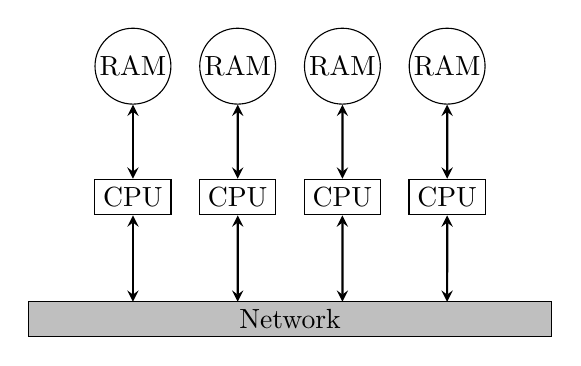
\begin{tikzpicture}[scale=1.33,>=stealth]
      \node[draw, inner sep=3pt] (P0) at (0, 1)  {CPU};
      \node[draw, inner sep=3pt] (P1) at (1, 1)  {CPU};
      \node[draw, inner sep=3pt] (P2) at (2, 1)  {CPU};
      \node[draw, inner sep=3pt] (P3) at (3, 1)  {CPU};

      \node[draw, shape=circle, inner sep=1pt] (R0) at (0, 2.25)  {RAM};
      \node[draw, shape=circle, inner sep=1pt] (R1) at (1, 2.25)  {RAM};
      \node[draw, shape=circle, inner sep=1pt] (R2) at (2, 2.25)  {RAM};
      \node[draw, shape=circle, inner sep=1pt] (R3) at (3, 2.25)  {RAM};

      \filldraw[fill=lightgray] (-1, 0) rectangle node (net) {Network} +(5, -0.33);

      \draw[<->,thick] (P0) edge (0, 0) edge (R0);
      \draw[<->,thick] (P1) edge (1, 0) edge (R1);
      \draw[<->,thick] (P2) edge (2, 0) edge (R2);
      \draw[<->,thick] (P3) edge (3, 0) edge (R3);
    \end{tikzpicture}
  \end{center}

  \begin{itemize}
  \item Each processor has its own memory
    
  \item Communication $=$ \alert{messages} exchanged on the network
  \end{itemize}
\end{frame}

%%%%%%%%%%%%%%%%%%%%%%%%%%%%%%%%%%%%%%%%%%%%%%%%%%%%%%%%%%%%%%%%%%%%%%%%%%%%%%%%%%%%

\begin{frame}
  \frametitle{Message Passing Interface}

  \begin{block}{In the early days}
    \begin{itemize}
    \item IBM, Cray, Silicon Graphics, ... had \textbf{their own} communication middleware
    \item Or course, \alert{not compatible} with each others
    \item Serious obstacle to code portability \triste
    \end{itemize}
  \end{block}

  \medskip
  
  \begin{exampleblock}{In 1994}
    \begin{itemize}
    \item v1.0 of the \textbf{MPI specification}
    \item Consortium with the usual suspects (Cray, IBM, ...)
    \item Goals:
      \begin{itemize}
      \item develop a widely used standard for writing message-passing programs.
      \item establish a practical, portable, efficient, and flexible standard
        for message-passing.
      \end{itemize}
    \end{itemize}
  \end{exampleblock}
\end{frame}

%%%%%%%%%%%%%%%%%%%%%%%%%%%%%%%%%%%%%%%%%%%%%%%%%%%%%%%%%%%%%%%%%%%%%%%%%%%%%%%%%%%%

\begin{frame}
  \frametitle{Some Context}

  \begin{itemize}
  \item Single Program / Multiple Data
  \item Many \textbf{processes}, all \alert{running the same code}
  \item Each process has a (unique) \textbf{rank}
  \end{itemize}

  \bigskip
  
  \begin{tikzpicture}
    \path[use as bounding box] (-1.5, -3) rectangle (9, 0.5);
    \begin{scope}[xshift=0cm]
      \node at (0, -0.5) {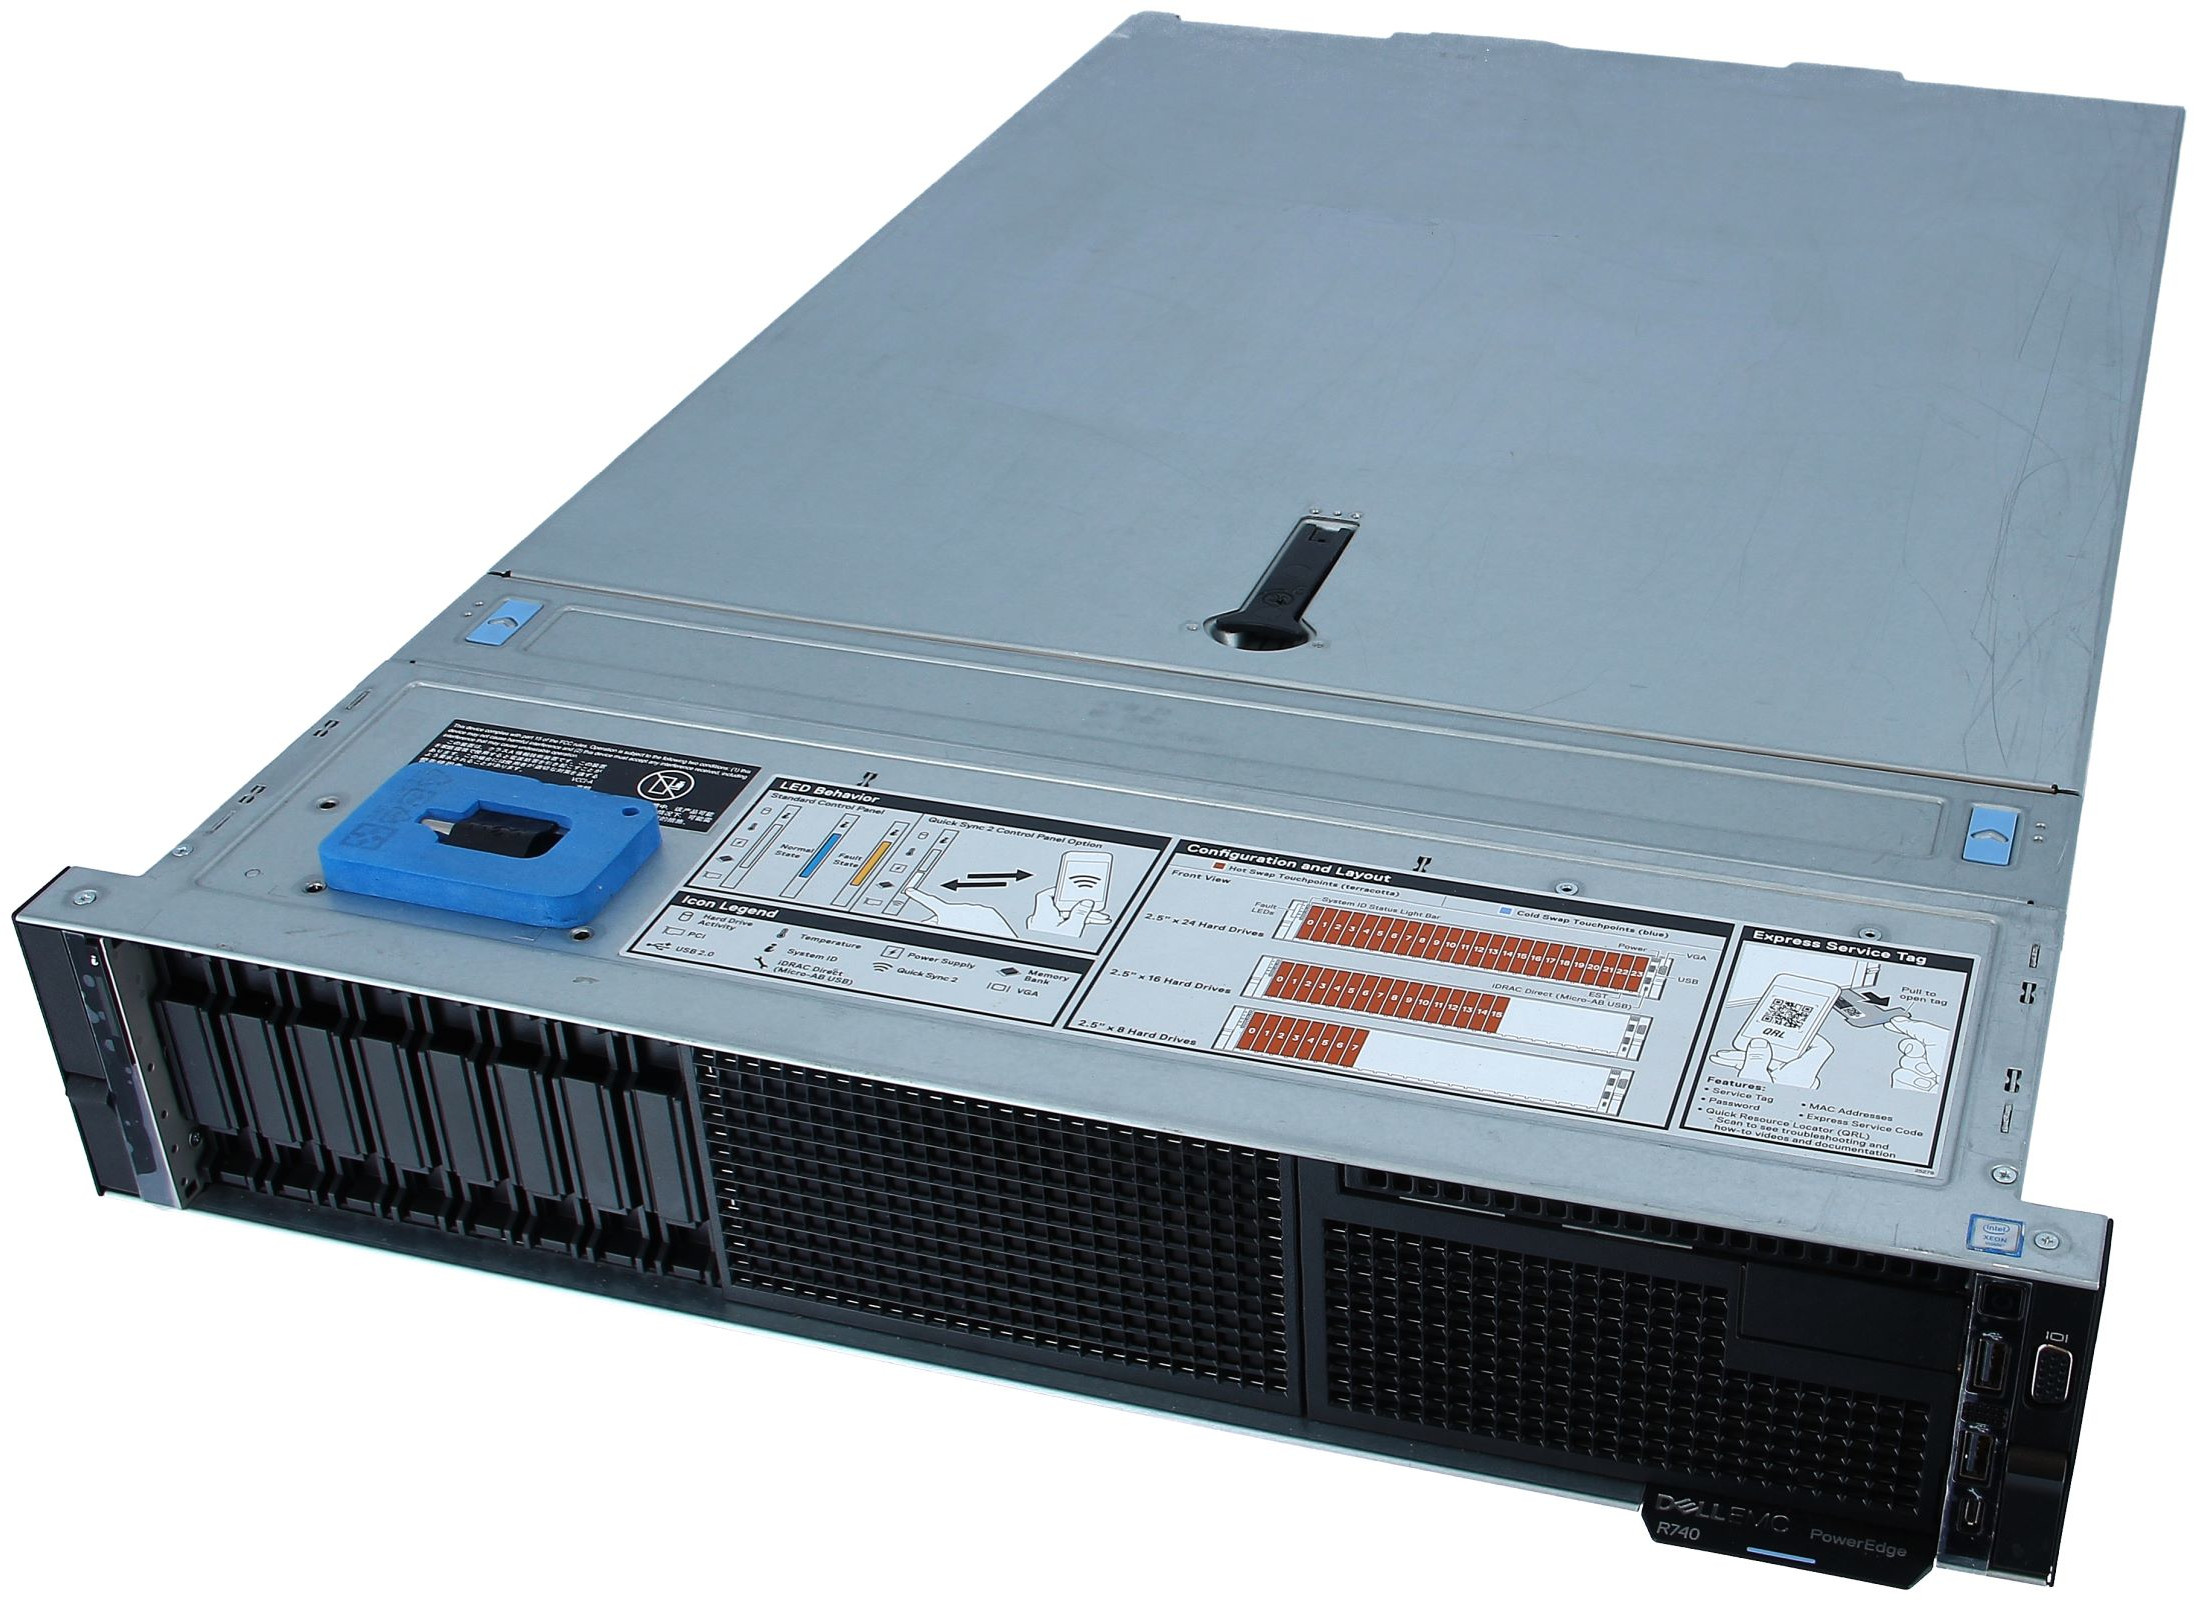
\includegraphics[width=3cm]{dell1}};
      \node<1>[inner sep=2pt, draw] at ( 0, -2) {$P_0$};
      
      \node<2,3>[inner sep=2pt, draw] at (-1, -2) {$P_0$};
      \node<2,3>[inner sep=2pt, draw] at ( 0, -2) {$P_1$};
      \node<2,3>[inner sep=2pt, draw] at ( 1, -2) {$P_2$};
      \node<2,3>[inner sep=2pt, draw] at (-1, -2.75) {$P_3$};
      \node<2,3>[inner sep=2pt, draw] at ( 0, -2.75) {$P_4$};
      \node<2,3>[inner sep=2pt, draw] at ( 1, -2.75) {$P_5$};
    \end{scope}

    \begin{scope}[xshift=3.75cm]
      \node<1,3> at (0, -0.5) {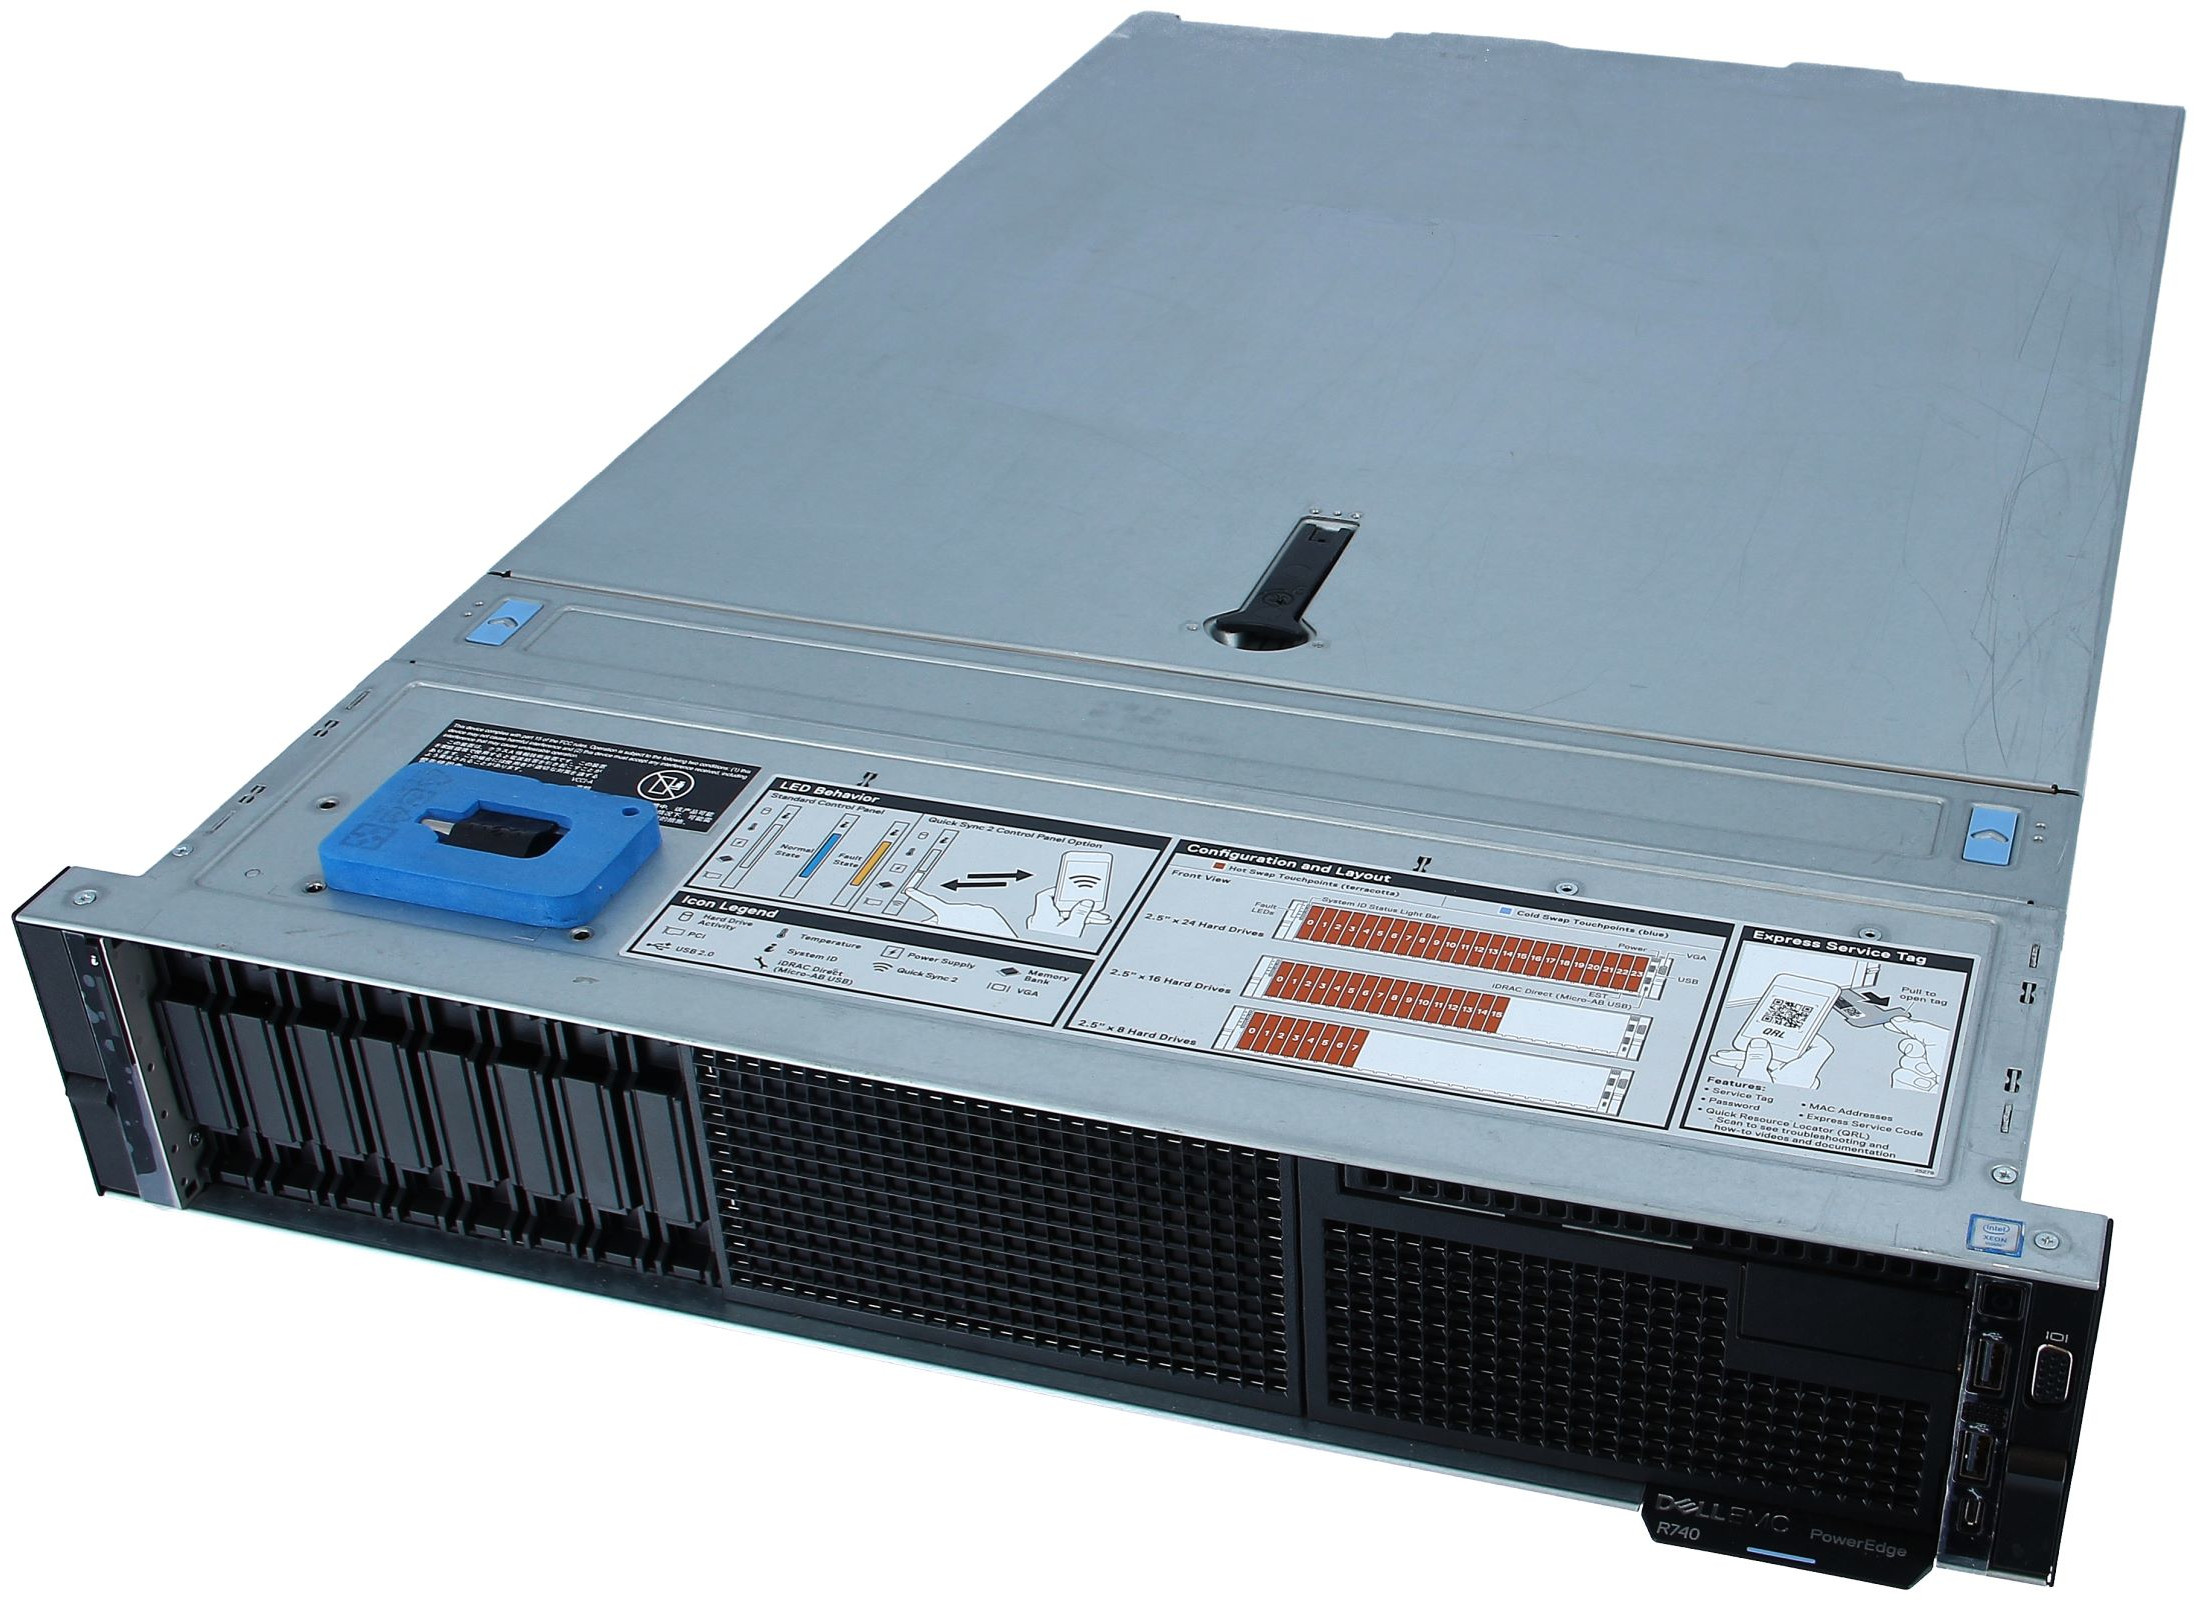
\includegraphics[width=3cm]{dell1}};
      \node<1>[inner sep=2pt, draw] at ( 0, -2) {$P_1$};

      \node<3>[inner sep=2pt, draw] at (-1, -2) {$P_6$};
      \node<3>[inner sep=2pt, draw] at ( 0, -2) {$P_7$};
      \node<3>[inner sep=2pt, draw] at ( 1, -2) {$P_8$};
      \node<3>[inner sep=2pt, draw] at (-1, -2.75) {$P_9$};
      \node<3>[inner sep=2pt, draw] at ( 0, -2.75) {$P_a$};
      \node<3>[inner sep=2pt, draw] at ( 1, -2.75) {$P_b$};
    \end{scope}

    \begin{scope}[xshift=7.5cm]
      \node<1,3> at (0, -0.5) {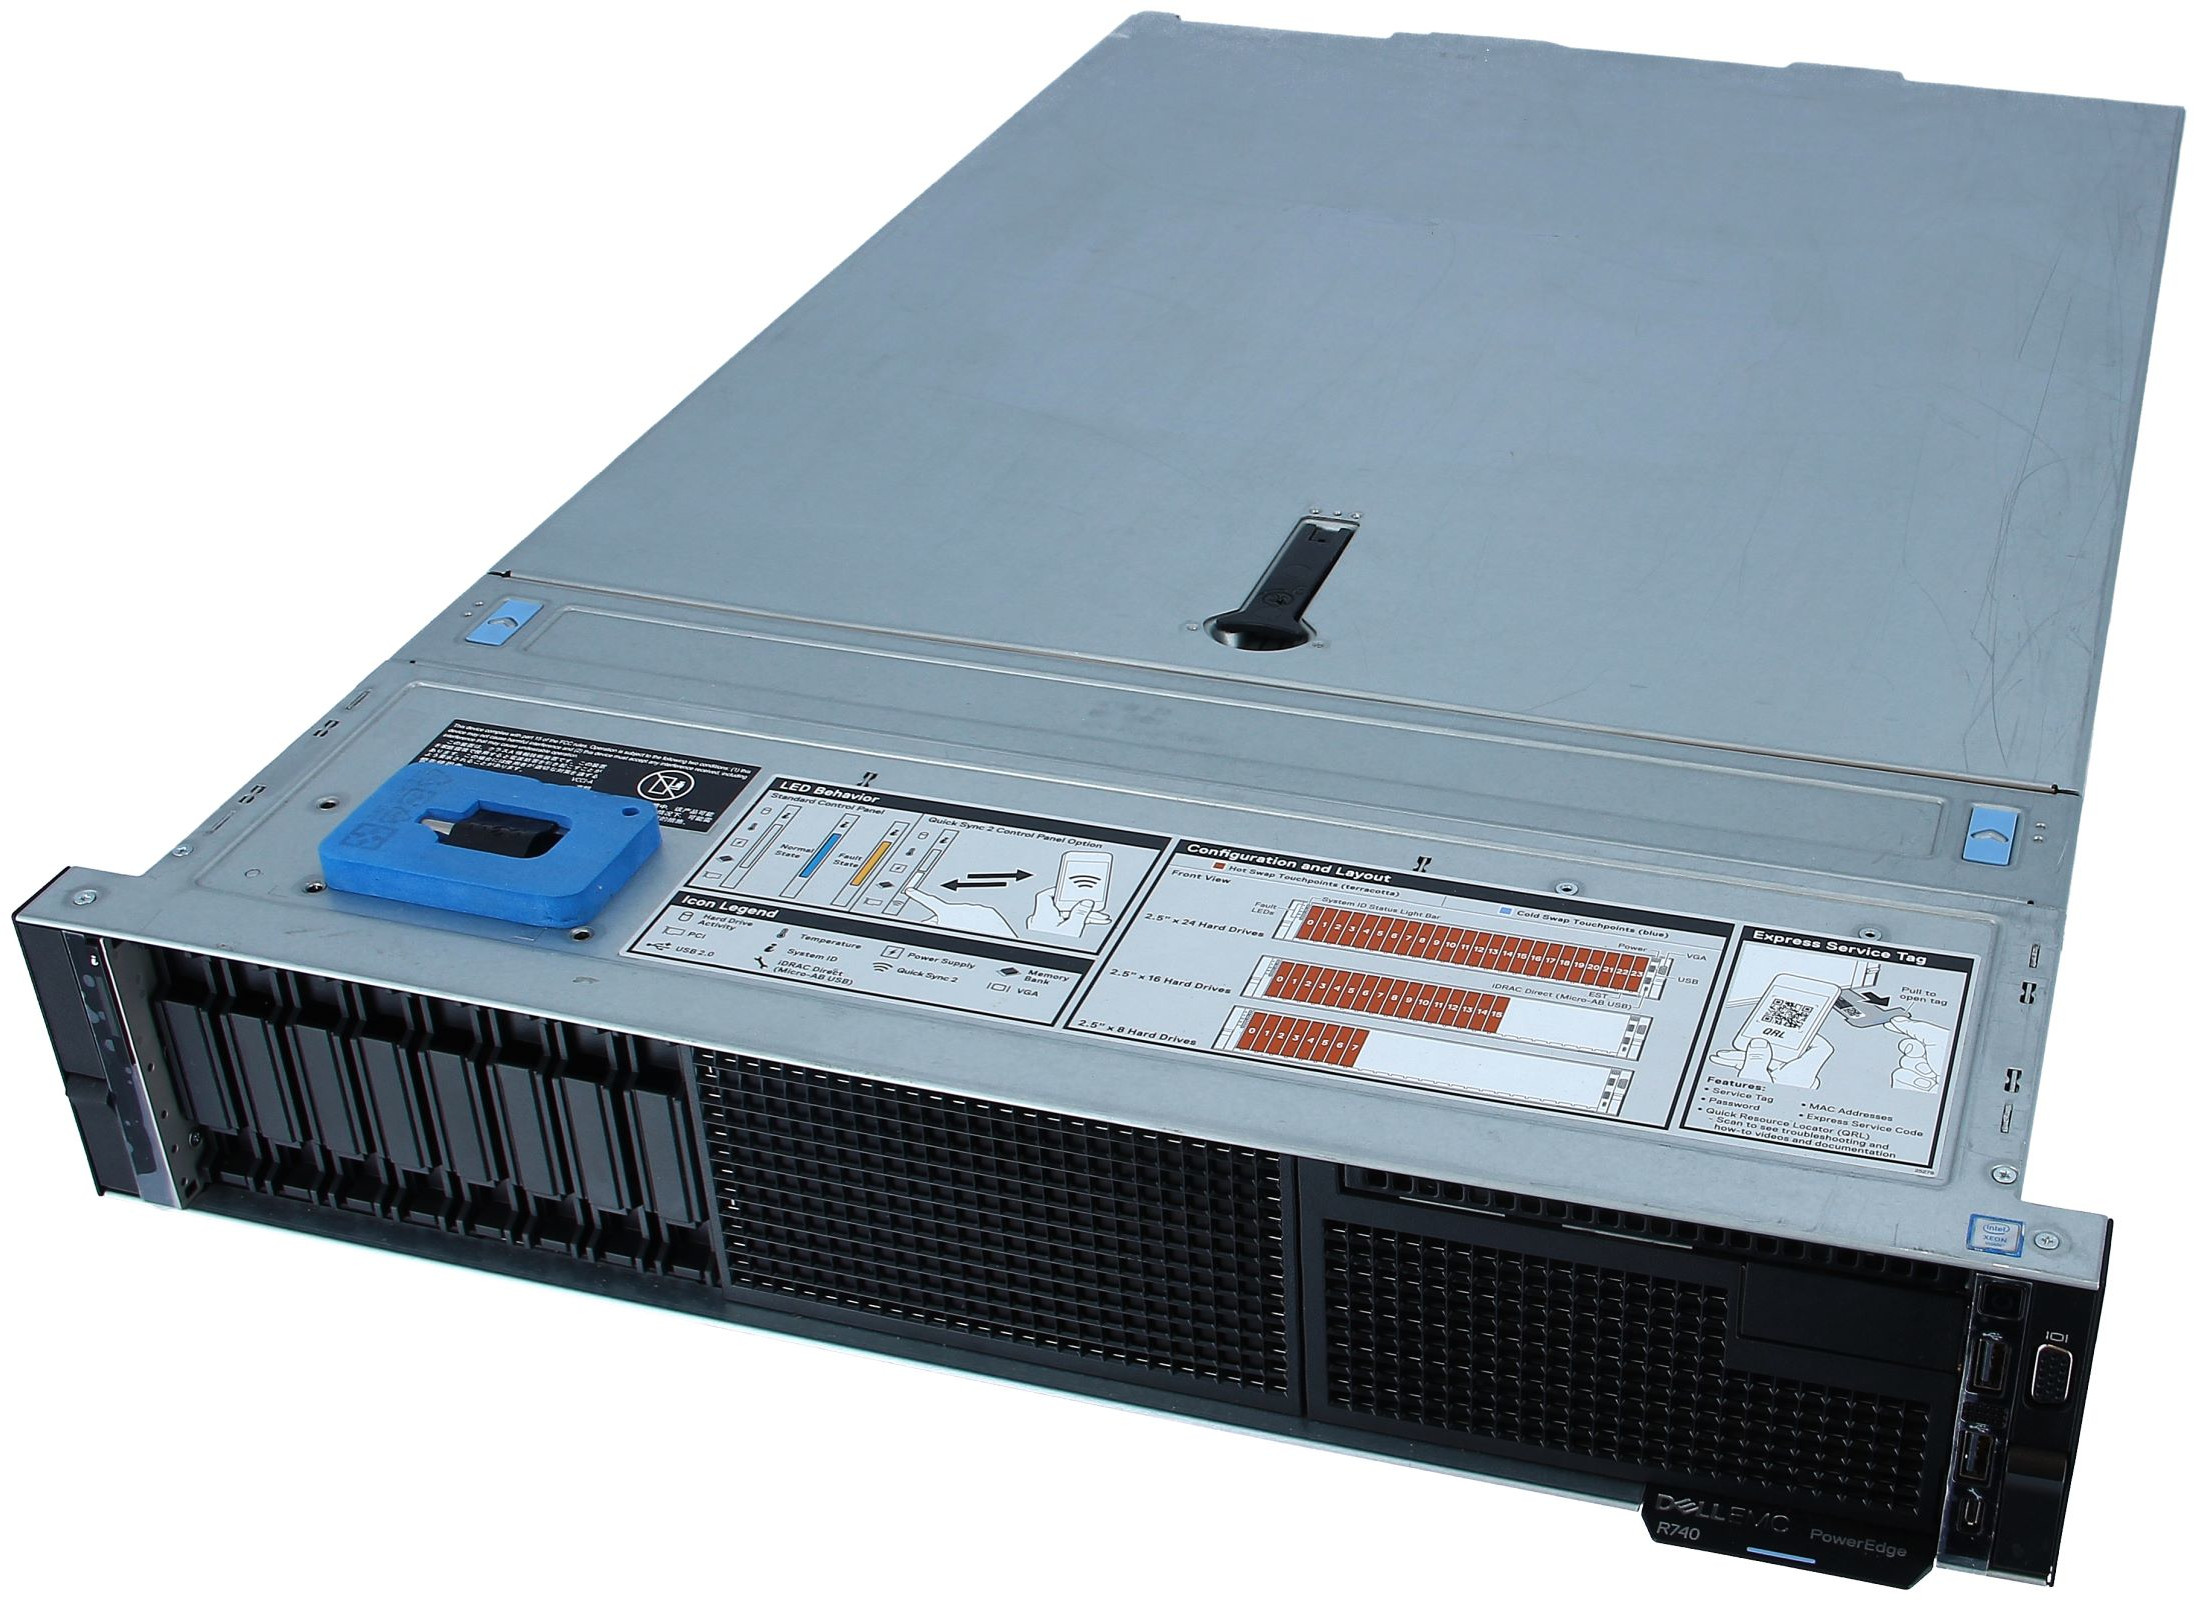
\includegraphics[width=3cm]{dell1}};
      \node<1>[inner sep=2pt, draw] at ( 0, -2) {$P_2$};

      \node<3>[inner sep=2pt, draw] at (-1, -2) {$P_c$};
      \node<3>[inner sep=2pt, draw] at ( 0, -2) {$P_d$};
      \node<3>[inner sep=2pt, draw] at ( 1, -2) {$P_e$};
      \node<3>[inner sep=2pt, draw] at (-1, -2.75) {$P_f$};
      \node<3>[inner sep=2pt, draw] at ( 0, -2.75) {$P_g$};
      \node<3>[inner sep=2pt, draw] at ( 1, -2.75) {$P_h$};
    \end{scope}
  \end{tikzpicture}

  \medskip
  
  \begin{itemize}
  \item Very flexible \& portable \smiley
  \end{itemize}

\end{frame}

%%%%%%%%%%%%%%%%%%%%%%%%%%%%%%%%%%%%%%%%%%%%%%%%%%%%%%%%%%%%%%%%%%%%%%%

\begin{frame}
  \frametitle{What MPI offers}

  \begin{alertblock}{1. Runtime Environment}
    \begin{itemize}
    \item The \texttt{mpiexec} program starts an MPI application
    \item Usual arguments
      \begin{itemize}
      \item Program to execute
      \item \# processes to start
      \item List of target nodes
      \item (optional) process placement directives
      \end{itemize}
    \end{itemize}
  \end{alertblock}

  \medskip
  
  \begin{exampleblock}{2. Library}
    \begin{itemize}
    \item \texttt{mpi.h} ($\approx 370$ functions...)
    \end{itemize}
  \end{exampleblock}

  \medskip

  \begin{block}{3. Compiler Wrapper}
    \begin{itemize}
    \item Use \texttt{mpicc} to compile MPI applications
      \begin{itemize}
      \item It invokes \texttt{gcc} with the right arguments 
      \end{itemize}
    \end{itemize}
  \end{block}
\end{frame}

%%%%%%%%%%%%%%%%%%%%%%%%%%%%%%%%%%%%%%%%%%%%%%%%%%%%%%%%%%%%%%%%%%%%%%

\begin{frame}[fragile=singleslide]
  \frametitle{MPI Startup and Termination}
    
\begin{minted}{C}
#include <mpi.h>

int main(int argc, char** argv)
{
    MPI_Init(&argc, &argv);

    /* your code goes here */
    
    MPI_Finalize();
}
\end{minted} 

\begin{block}{Dead Weight of History}
  \begin{itemize}
  \item \mintinline{C}{MPI_Init} used to inspect/modify \mintinline{C}{argc, argv} in early MPI implementations
  \item It is \alert{legal} (and simpler) to call \mintinline{C}{MPI_Init(NULL, NULL);}
  \end{itemize}
\end{block}
\end{frame}

%%%%%%%%%%%%%%%%%%%%%%%%%%%%%%%%%%%%%%%%%%%%%%%%%%%%%%%%%%%%%%%%%%%%%

\begin{frame}[fragile=singleslide]
  \frametitle{MPI Startup and Termination}

  \begin{exampleblock}{Library functions}
    \begin{itemize}
    \item \mintinline{C}{int MPI_Init(int *argc, char ***argv)}
    \item \mintinline{C}{int MPI_Finalize()}
    \end{itemize}
  \end{exampleblock}

  \begin{block}{Remarks}
    \begin{itemize}
    \item (almost) All MPI functions return an \alert{error code}
    \item Default MPI error handler = $\skull$ \textbf{KILL} $\skull$ your application
      \begin{itemize}
      \item[$\leadsto$] No need to check the error codes...
      \end{itemize}
    \item Default behavior can be changed
    \end{itemize}
  \end{block}
  
\end{frame}

%%%%%%%%%%%%%%%%%%%%%%%%%%%%%%%%%%%%%%%%%%%%%%%%%%%%%%%%%%%%%%%%%%%%%%

\begin{frame}[fragile]
  \frametitle{Communicators}

  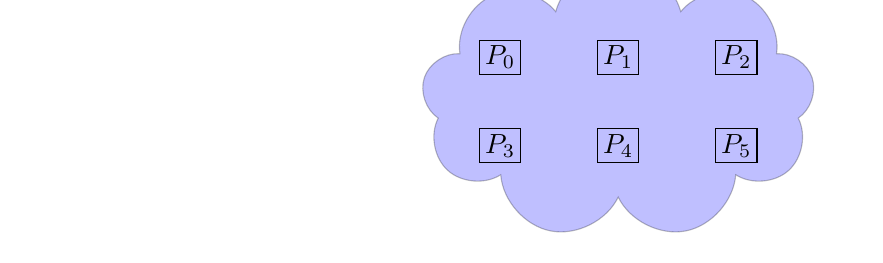
\begin{tikzpicture}[scale=1.5]
    \path[use as bounding box] (-5, -3.5) rectangle (2, -1.75);
    \node [cloud, cloud puffs=9, draw, minimum width=5cm, minimum height=3.5cm, fill=blue, nearly transparent] at (0, -2.375) {};
    
    \node[inner sep=2pt, draw] at (-1, -2) {$P_0$};
    \node[inner sep=2pt, draw] at ( 0, -2) {$P_1$};
    \node[inner sep=2pt, draw] at ( 1, -2) {$P_2$};
    \node[inner sep=2pt, draw] at (-1, -2.75) {$P_3$};
    \node[inner sep=2pt, draw] at ( 0, -2.75) {$P_4$};
    \node[inner sep=2pt, draw] at ( 1, -2.75) {$P_5$};
    \end{tikzpicture}

      \begin{itemize}
      \item Process group + communication context
        \begin{itemize}
        \item Ranks start at zero
        \end{itemize}
      \item Opaque object of type \mintinline{C}{MPI_Comm}
      \item On startup, \mintinline{C}{MPI_COMM_WORLD} contains all processes
      \item (advanced technique) new communicators can be created
      \end{itemize}

    \begin{exampleblock}{MPI Library functions}
    \begin{itemize}
    \item \mintinline{C}{int MPI_Comm_size(MPI_Comm comm, int *size)}
    \item \mintinline{C}{int MPI_Comm_rank(MPI_Comm comm, int *rank)}
    \end{itemize}
  \end{exampleblock}
\end{frame}

%%%%%%%%%%%%%%%%%%%%%%%%%%%%%%%%%%%%%%%%%%%%%%%%%%%%%%%%%%%%%%%%%%%%%%%%%%%%%%%%%%%%

\begin{frame}
  \frametitle{Messages}

  \begin{itemize}
  \item \textbf{data} (\alert{array} of values) + \textbf{envelope} (``metadata'')
  \end{itemize}
  
  \begin{alertblock}{Message data}
    \begin{description}
    \item[buffer]    Memory address of the first element
    \item[count]     Number of elements
    \item[datatype]  Type of the elements
    \end{description}
  \end{alertblock}

  \begin{block}{Envelope}
    \begin{description}
    \item[source]       rank of the sending process
    \item[destination]  rank of the receiving process
    \item[tag]          arbitrary integer (``nature'' of the message)
    \item[communicator] messages belong to a single communicator
    \end{description}
  \end{block}
\end{frame}

%%%%%%%%%%%%%%%%%%%%%%%%%%%%%%%%%%%%%%%%%%%%%%%%%%%%%%%%%%%%%%%%%%%%%%%%%%%%%%%%%%%

\begin{frame}[fragile=singleslide]
  \frametitle{Basic Data Types}

  \begin{center}
\begin{tabular}{|l|l|}
\hline
  MPI type & C type \\
\hline
\hline
\mintinline{C}{MPI_CHAR} & \mintinline{C}{char} \\
\hline
\mintinline{C}{MPI_SHORT} & \mintinline{C}{short int} \\
\hline
\mintinline{C}{MPI_INT} & \mintinline{C}{int} \\
\hline
\mintinline{C}{MPI_LONG} & \mintinline{C}{long} \\
\hline
\mintinline{C}{MPI_LONG_LONG_INT} & \mintinline{C}{long long int} \\
\hline
\mintinline{C}{MPI_FLOAT} & \mintinline{C}{float} \\
\hline
\mintinline{C}{MPI_DOUBLE} & \mintinline{C}{double} \\
\hline
\mintinline{C}{MPI_LONG_DOUBLE} & \mintinline{C}{long double} \\
\hline
\mintinline{C}{MPI_INT8_T} & \mintinline{C}{int8_t} \\
\hline
\mintinline{C}{MPI_INT16_T} & \mintinline{C}{int16_t} \\
\hline
\mintinline{C}{MPI_INT32_T} & \mintinline{C}{int32_t} \\
\hline
\mintinline{C}{MPI_INT64_T} & \mintinline{C}{int64_t} \\
\hline
\mintinline{C}{MPI_BYTE} & \\
\hline
\end{tabular}
\end{center}
\end{frame}

%%%%%%%%%%%%%%%%%%%%%%%%%%%%%%%%%%%%%%%%%%%%%%%%%%%%%%%%%%%%%%%%%%%%%%%%%%%%%%%%%%%%%%%%%%%%%%

\begin{frame}[fragile]
  \frametitle{Point-to-Point Communication}

  \begin{tikzpicture}
    \begin{scope}[xshift=0cm]
      \node at (0, -0.5) {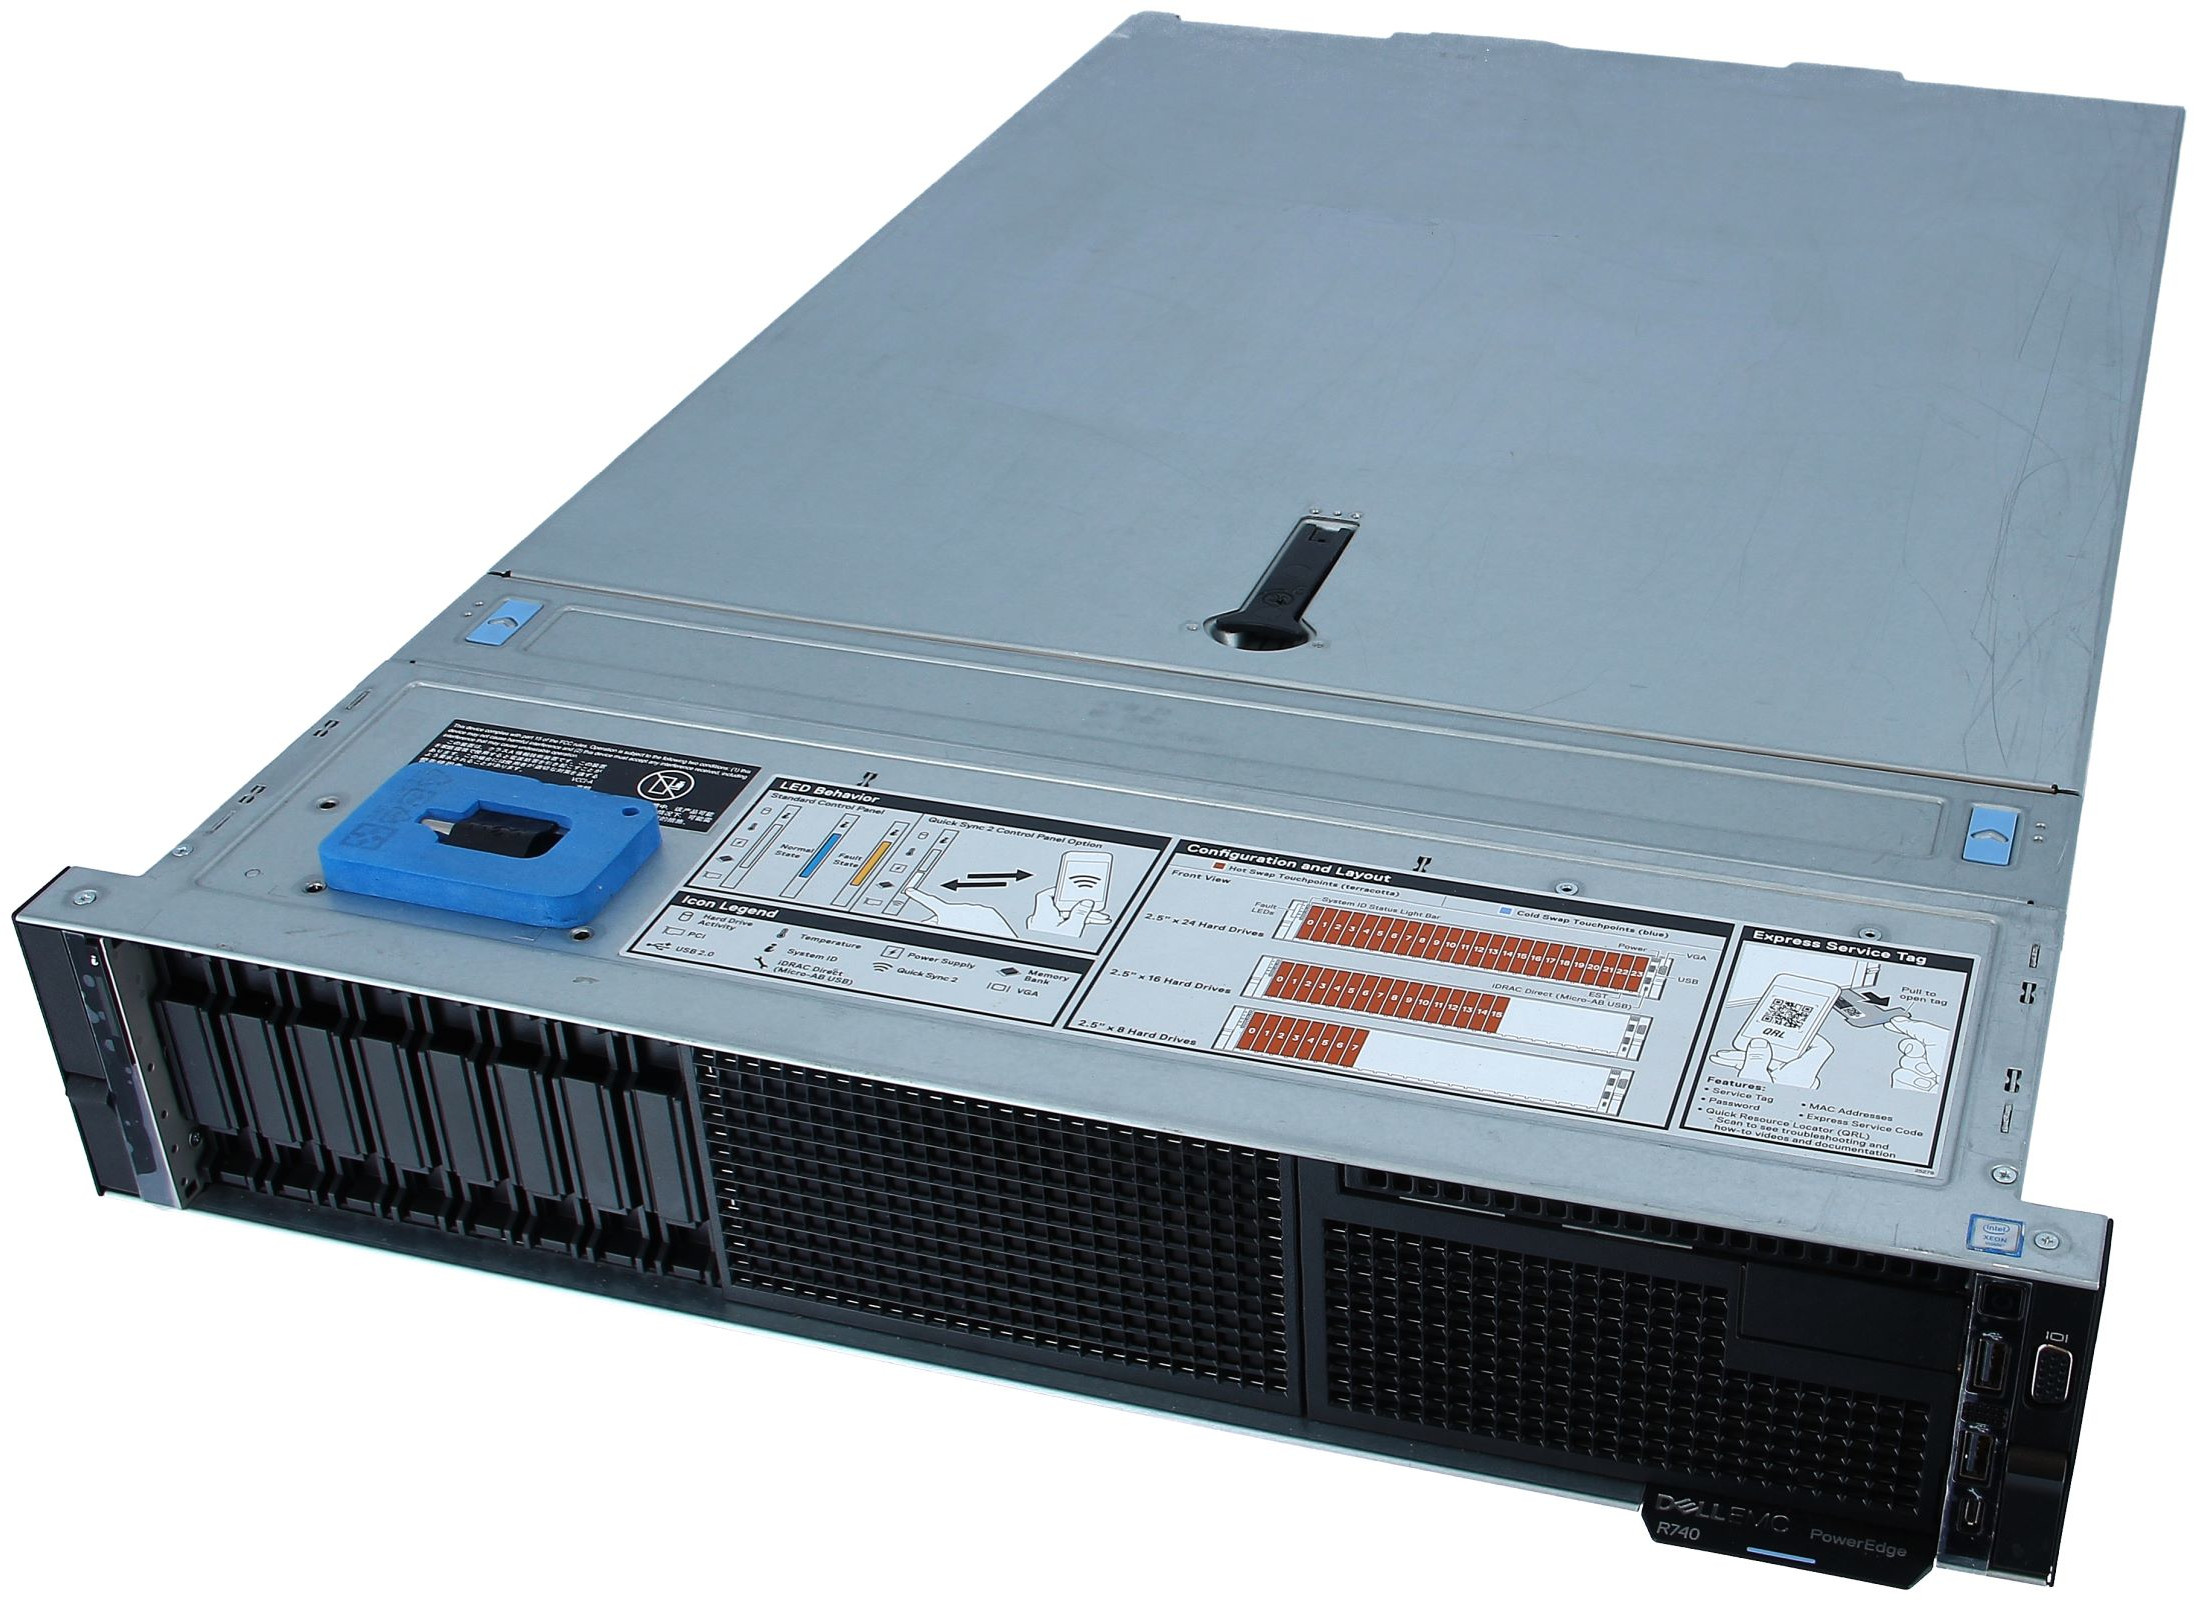
\includegraphics[width=3cm]{dell1}};
      \node[inner sep=2pt, draw] at ( 0, -2) (Pi) {$P_i$};
      \draw (Pi) -- (0, -2.5);
      \draw[fill=blue, semitransparent] (-1, -2.5) rectangle (1, -6);
      \draw[fill=yellow!50] (-0.9, -3) rectangle node {data} +(1.8, -1);
      \node[white, anchor=south] at (0, -6) {memory};
      \node[] at (0, -7) {\mintinline{C}{send(...)}};
    \end{scope}

    \begin{scope}[xshift=7cm]
      \node at (0, -0.5) {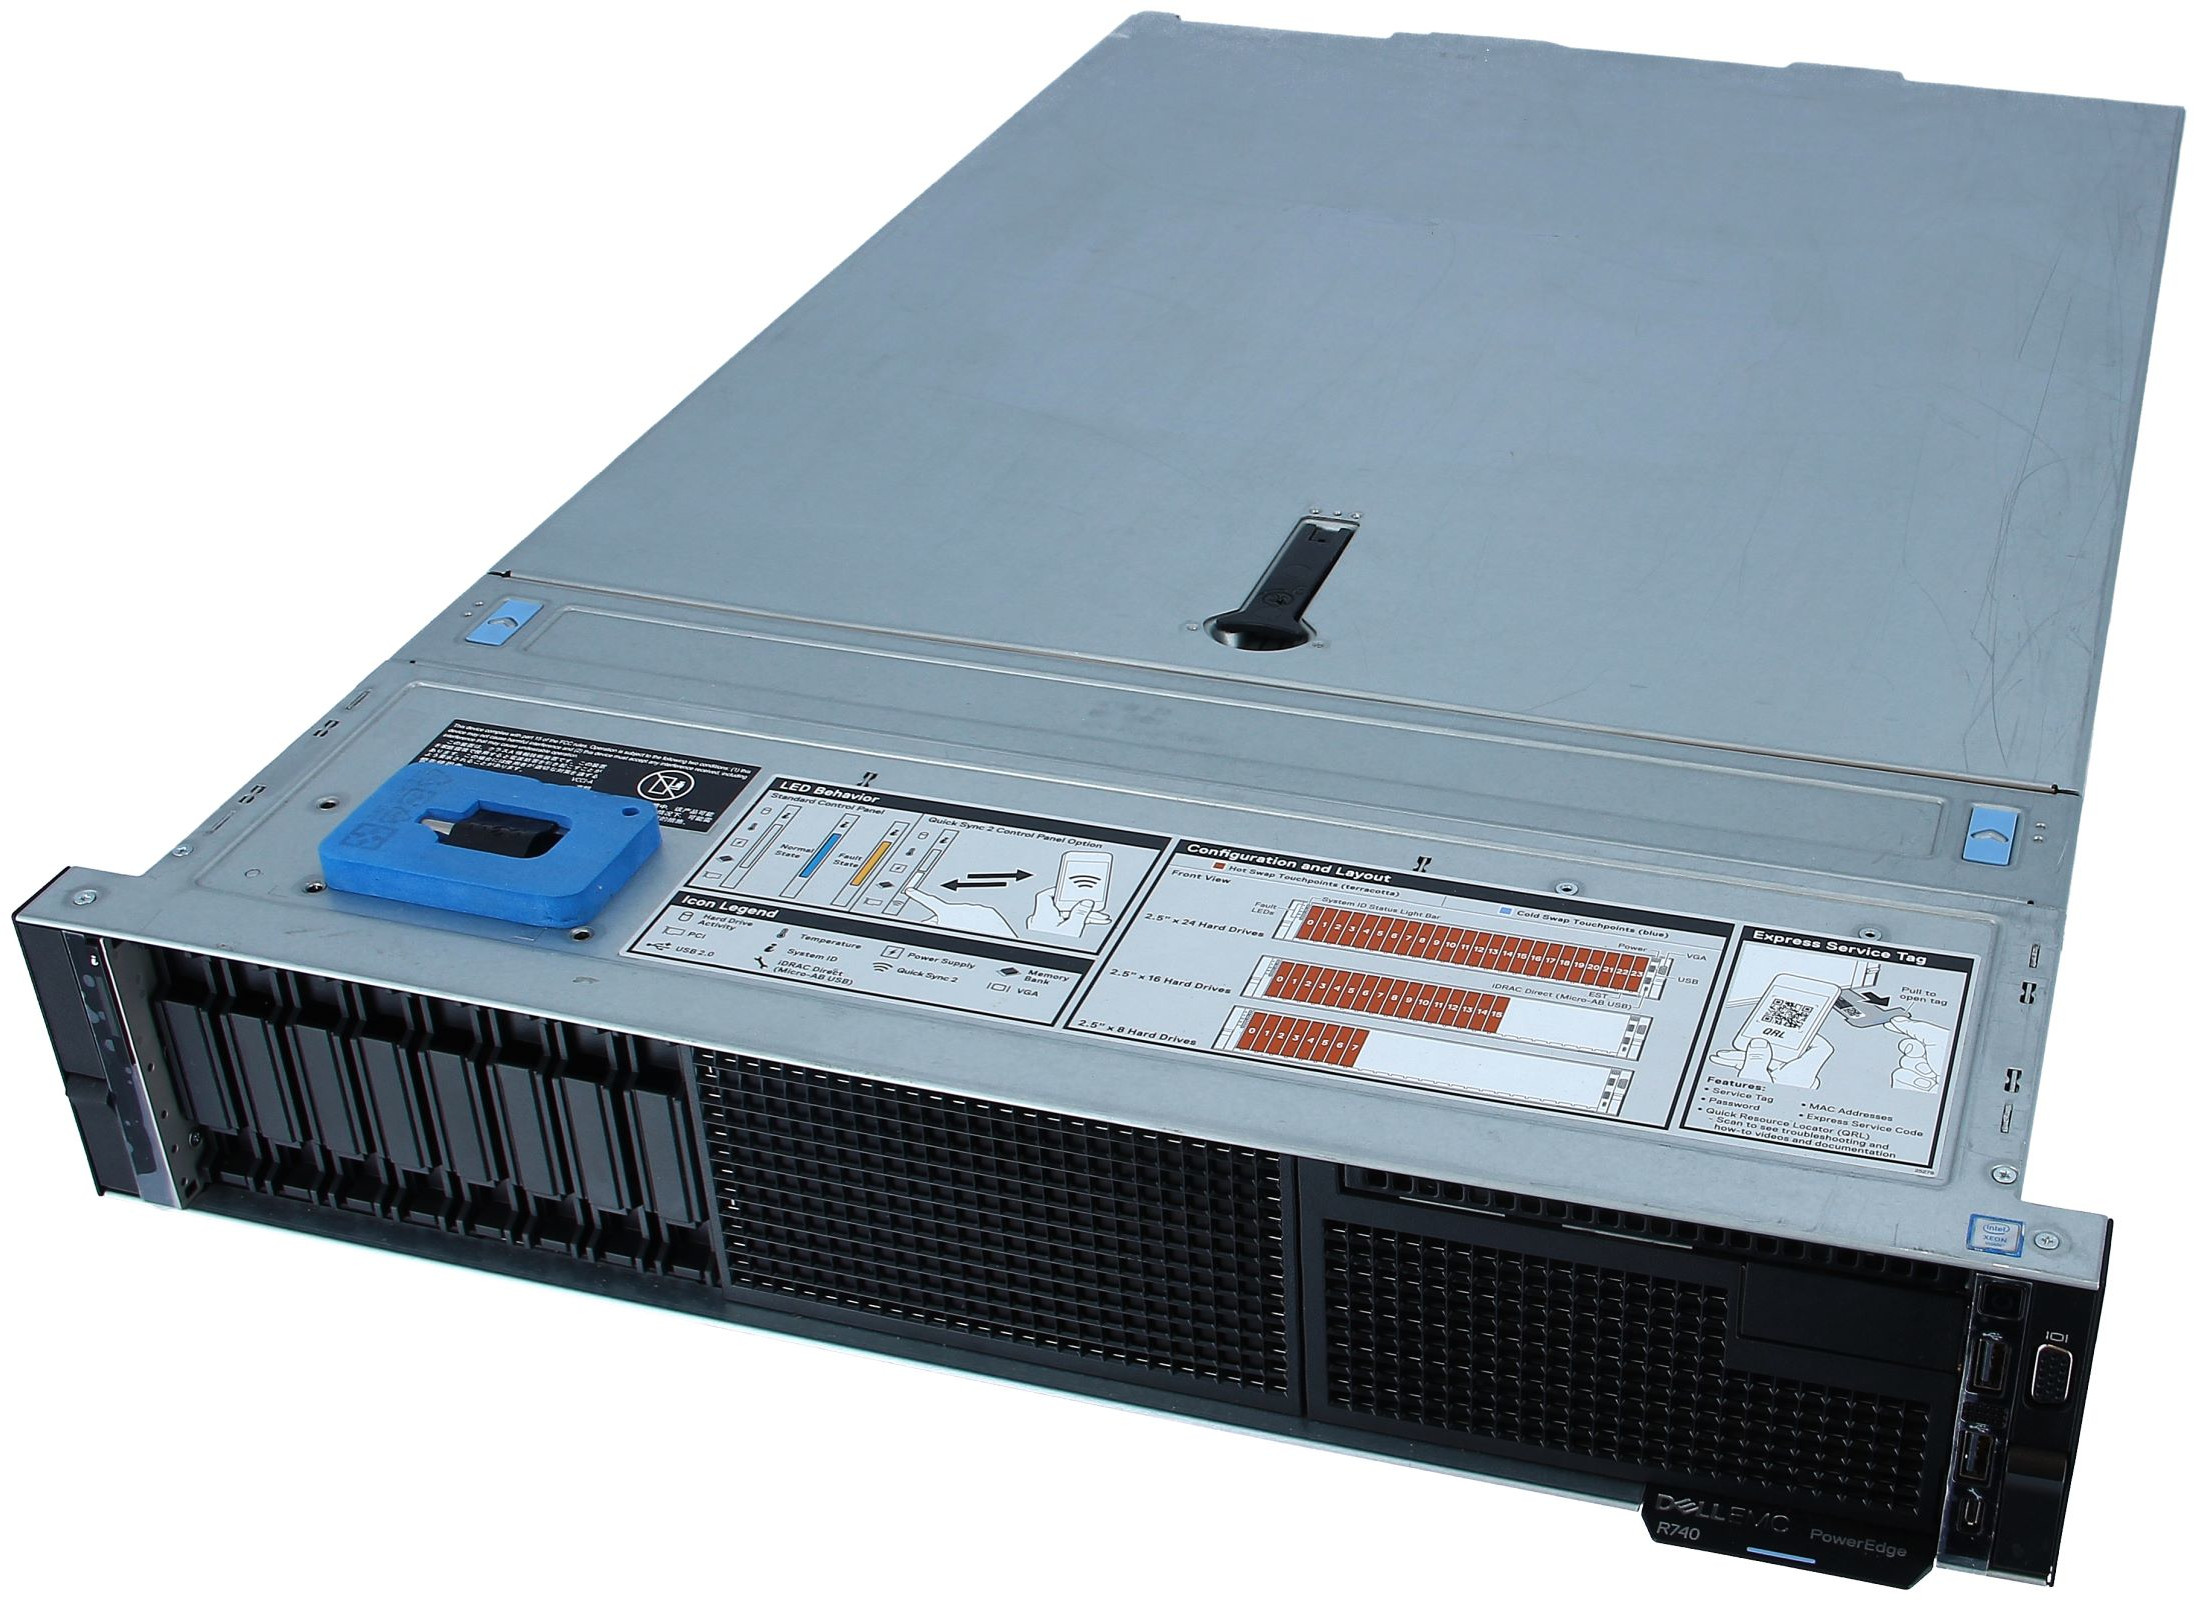
\includegraphics[width=3cm]{dell1}};
      \node[inner sep=2pt, draw] at ( 0, -2) (Pj) {$P_j$};
      \draw (Pj) -- (0, -2.5);
      \draw[fill=blue, semitransparent] (-1, -2.5) rectangle  (1, -6);
      \draw[fill=yellow!50] (-0.9, -4) rectangle node {\only<3>{data}} +(1.8, -1);
      \node[white, anchor=south] at (0, -6) {memory};
      \node[] at (0, -7) {\mintinline{C}{recv(...)}};
    \end{scope}

    \draw<2>[red,ultra thick, ->] (1, -3.5) -- (2, -3.5) -- (5, -4.5) -- (6, -4.5);
  \end{tikzpicture}  
\end{frame}

%%%%%%%%%%%%%%%%%%%%%%%%%%%%%%%%%%%%%%%%%%%%%%%%%%%%%%%%%%%%%%%%%%%%%%%%%%%%%%%%%%%%%%%%%%%%%%%

\begin{frame}[fragile=singleslide]
  \frametitle{Point-to-Point Communication (sending)}

\begin{minted}[fontsize=\small]{C}
int MPI_Send(void* buf, int count, MPI_Datatype datatype,
             int dest, int tag, MPI_Comm comm)
\end{minted}

  \begin{block}{Comments}
    \begin{itemize}
    \item Read a message in memory from \alert{send buffer}
      \begin{itemize}
      \item \mintinline{C}{count} elements of type \mintinline{C}{datatype} at address \mintinline{C}{buf}      
      \end{itemize}
    \item Send it to process of rank \mintinline{C}{dest} in communicator \mintinline{C}{comm}
    \item Message ``labelled'' with \mintinline{C}{tag}
      \begin{itemize}
      \item $0 \leq \mintinline{C}{tag} < 2^{15} \leq $
      \end{itemize}
    \item Function returns when message has been entirely read
      \begin{itemize}
      \item The send buffer can be safely overwritten
      \end{itemize}
    \end{itemize}
  \end{block}
\end{frame}

%%%%%%%%%%%%%%%%%%%%%%%%%%%%%%%%%%%%%%%%%%%%%%%%%%%%%%%%%%%%%%%%%%%%%%%%%%%%%%%%%%%%%%%%%%%%%%%

\begin{frame}[fragile=singleslide]
  \frametitle{Point-to-Point Communication (sending)}

\begin{minted}[fontsize=\small]{C}
int MPI_Send(void* buf, int count, MPI_Datatype datatype,
             int dest, int tag, MPI_Comm comm)
\end{minted}

  \begin{alertblock}{MPI data types}
    \begin{itemize}
    \item With basic datatypes:
      \begin{itemize}
      \item Message = array of \textbf{contiguous} values in memory
      \end{itemize}

    \item Create more complex MPI types using MPI functions
      \begin{itemize}
      \item Array of \mintinline{C}{struct}
      \item Non-contiguous (jumps between values)
      \item See MPI spec ; out of the scope of this lecture
      \end{itemize}
    \end{itemize}
  \end{alertblock}
\end{frame}

%%%%%%%%%%%%%%%%%%%%%%%%%%%%%%%%%%%%%%%%%%%%%%%%%%%%%%%%%%%%%%%%%%%%% 

\begin{frame}[fragile=singleslide]
  \frametitle{Point-to-Point Communication (receiving)}

\begin{minted}[fontsize=\small]{C}
int MPI_Recv(void* buf, int count, MPI_Datatype datatype,
             int source, int tag, MPI_Comm comm,
             MPI_Status *status)
\end{minted}

  \begin{block}{Comments about \mintinline{C}{MPI_Recv}}
    \begin{itemize}
    \item Wait for \alert{matching} message
      \begin{itemize}
      \item Labelled \mintinline{C}{tag} from process \mintinline{C}{source} in communicator \mintinline{C}{comm}
      \end{itemize}
    \item Write it in memory in \alert{receive buffer} (at address \mintinline{C}{status})
    \item Write metadata in \mintinline{C}{status}
    \item Size of the message must be $\leq$ \mintinline{C}{count}
      \begin{itemize}
      \item Actual number of received values may be smaller
      \end{itemize}    
    \end{itemize}
  \end{block}
\end{frame}

%%%%%%%%%%%%%%%%%%%%%%%%%%%%%%%%%%%%%%%%%%%%%%%%%%%%%%%%%%%%%%%%%%%%%%%%%%%%%%%%%%%%%%%%%%%%%%%%%%%

\begin{frame}[fragile=singleslide]
  \frametitle{Point-to-Point Communication (receiving, continued)}

\begin{minted}[fontsize=\small]{C}
int MPI_Recv(void* buf, int count, MPI_Datatype datatype,
             int source, int tag, MPI_Comm comm,
             MPI_Status *status)
\end{minted}

  \begin{block}{Can use \textbf{wildcards}}
    \begin{itemize}
      \item \mintinline{C}{tag == MPI_ANY_TAG}
      \item \mintinline{C}{source == MPI_ANY_SOURCE}
      \end{itemize}
    \end{block}

    \begin{exampleblock}{Inspecting metadata in \mintinline{C}{status}}
      \begin{itemize}
      \item Not written if \mintinline{C}{status == MPI_STATUS_IGNORE}
      \item \mintinline{C}{MPI_status} is a \mintinline{C}{struct}
        \begin{itemize}
        \item fields \mintinline{C}{MPI_SOURCE} and \mintinline{C}{MPI_TAG}
        \end{itemize}
        \vspace{-3mm}%
      \item \begin{minted}[fontsize=\small]{C}
int MPI_Get_count(MPI_Status *status,
                  MPI_Datatype datatype, int *count)
\end{minted}
        \vspace{-5mm}
\end{itemize}
    \end{exampleblock}
\end{frame}

%%%%%%%%%%%%%%%%%%%%%%%%%%%%%%%%%%%%%%%%%%%%%%%%%%%%%%%%%%%%%%%%%%%%%%%%%%%%%%%%%%%%%%%%

\begin{frame}
  \frametitle{Semantics of Point-to-Point Communication}

  \begin{itemize}
  \item Messages are not lost
  \item Messages are not duplicated
  \item Messages do not overtake
    \begin{itemize}
    \item $P_i$ sends two messages $M$, $M'$ in succession to $P_j$
    \item $P_j$ posts a receive maching both messages
    \item $P_j$ receives $M$ first 
    \end{itemize}
  \item \alert{No guarantees when senders are different}
    \begin{itemize}
    \item Inherent nondeterminism
    \end{itemize}
  \end{itemize}

  \begin{center}
  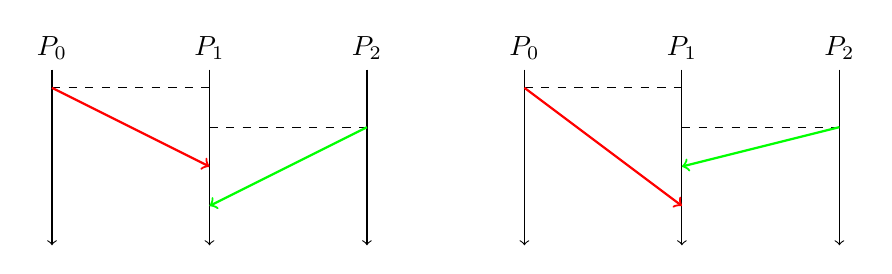
\begin{tikzpicture}[yscale=0.5, xscale=2]
    \begin{scope}
      \node at (-1, 5) (P1) {$P_0$};
      \node at (0, 5) (P2) {$P_1$};
      \node at (1, 5) (P3) {$P_2$};
      \draw (P1) edge[->] (-1, 0);
      \draw (P2) edge[->] ( 0, 0);
      \draw (P3) edge[->] ( 1, 0);
      \draw[dashed] (-1, 4) -- (0, 4);
      \draw[dashed] (0, 3) -- (1, 3);
      \draw[red, thick, ->] (-1, 4) -- (0, 2);
      \draw[green, thick, ->] (1, 3) -- (0, 1);
    \end{scope}
    \begin{scope}[xshift=3cm]
      \node at (-1, 5) (P1) {$P_0$};
      \node at (0, 5) (P2) {$P_1$};
      \node at (1, 5) (P3) {$P_2$};
      \draw (P1) edge[->] (-1, 0);
      \draw (P2) edge[->] ( 0, 0);
      \draw (P3) edge[->] ( 1, 0);
      \draw[dashed] (-1, 4) -- (0, 4);
      \draw[dashed] (0, 3) -- (1, 3);
      \draw[red, thick, ->] (-1, 4) -- (0, 1);
      \draw[green, thick, ->] (1, 3) -- (0, 2);
    \end{scope}  
  \end{tikzpicture}
\end{center}
\end{frame}

%%%%%%%%%%%%%%%%%%%%%%%%%%%%%%%%%%%%%%%%%%%%%%%%%%%%%%%%%%%%%%%%%%%

\begin{frame}
  \frametitle{Minimal MPI}

  \begin{itemize}
  \item \mintinline{C}{MPI_Init()}
  \item \mintinline{C}{MPI_Comm_size()}
  \item \mintinline{C}{MPI_Comm_rank()}
  \item \mintinline{C}{MPI_Send()}
  \item \mintinline{C}{MPI_Recv()}    
  \item \mintinline{C}{MPI_Finalize()}
  \end{itemize}

  \begin{alertblock}{Major advantage}
    \begin{itemize}
    \item Works over any kind of weird network
    \end{itemize}
  \end{alertblock}
\end{frame}

%%%%%%%%%%%%%%%%%%%%%%%%%%%%%%%%%%%%%%%%%%%%%%%%%%%%%%%%%%%%%%%%%%

\begin{frame}[fragile=singleslide]
\frametitle{MPI Speed on Grid5000}

\begin{minted}[fontsize=\small]{C}
int MPI_Send(void* buf, int count, MPI_Datatype datatype,
             int dest, int tag, MPI_Comm comm);

int MPI_Recv(void* buf, int count, MPI_Datatype datatype,
             int source, int tag, MPI_Comm comm,
             MPI_Status *status);
\end{minted}

\bigskip

\footnotesize 
\begin{tabular}{|c|c|c|l|r|r|}
  \hline
  Cluster & Site & Year & Interconnect & Bandwith & Latency \\
  \hline
  \hline
  PPTI      & jussieu & 20?? & \phantom{00}1Gbit ethernet &    64MB/s & 50.0$\mu$s \\
  sagitaire & lyon  & 2006 & \phantom{00}1Gbit ethernet   &   116MB/s & 65.0$\mu$s \\
  taurus    & lyon  & 2012 & \phantom{0}10Gbit ethernet   &  1156MB/s & 25.9$\mu$s\\
  gros      & nancy & 2019 & \phantom{0}25Gbit ethernet   &  2480MB/s & 8.9$\mu$s\\
  \hline
  grcinq    & nancy & 2013 & \phantom{0}56Gbit InfiniBand &  2488MB/s & 1.2$\mu$s \\
  grimoire  & nancy & 2016 & \phantom{0}56Gbit InfiniBand &  4248MB/s & 1.1$\mu$s\\
  drac      & grenoble & 2015 & 100Gbit InfiniBand        &  7760MB/s & 1.7$\mu$s \\
  \hline
  grvingt   & nancy & 2018 & 100Gbit OmniPath             & 12100MB/s & 0.9$\mu$s \\
  \hline
\end{tabular}


(measure : ping-pong between two nodes)
\end{frame}


%%%%%%%%%%%%%%%%%%%%%%%%%%%%%%%%%%%%%%%%%%%%%%%%%%%%%%%%%%%%%%%%%

\begin{frame}[fragile=singleslide]
  \frametitle{Blocking Receive}

  \begin{tikzpicture}[xscale=0.8]
    \path[use as bounding box] (-3.5, -6) rectangle (10.5, 0.5);
    \begin{scope}[xshift=0cm, yscale=1]
      \node at (0, -0.5) {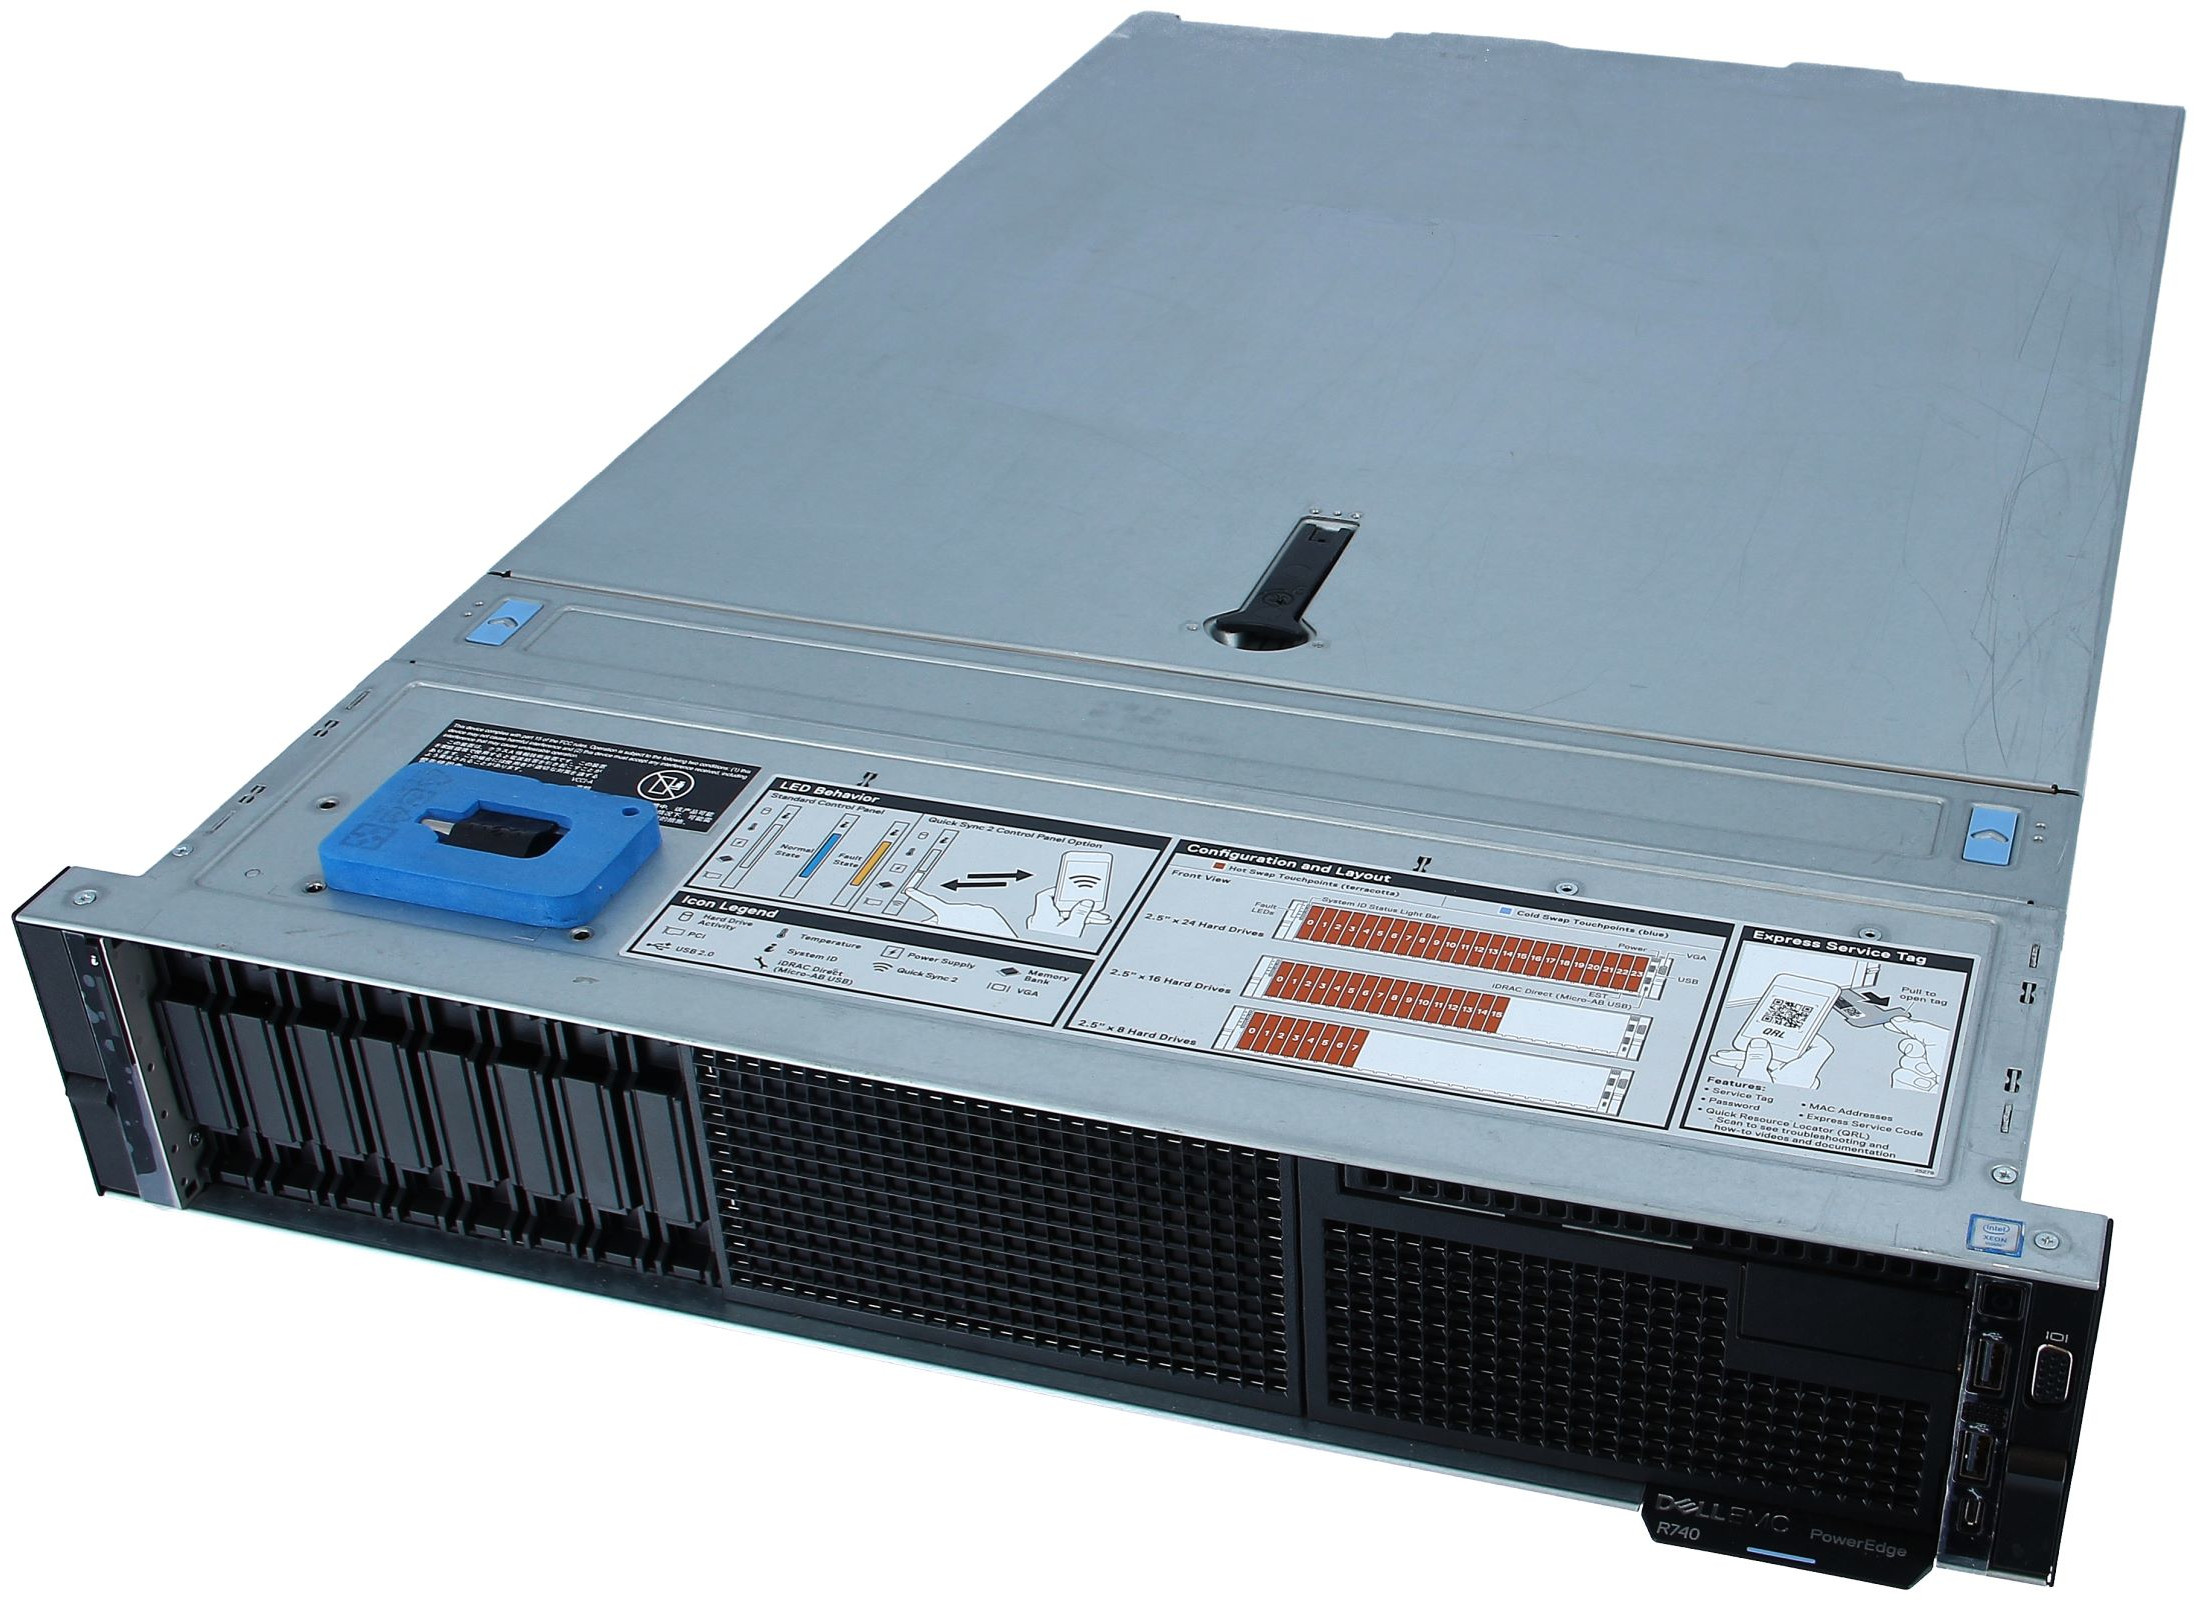
\includegraphics[width=3cm]{dell1}};
      \node[inner sep=2pt, draw] at ( 0, -2) (Pi) {$P_i$};
      \draw (Pi) -- (0, -2.5);
      \draw[fill=green] (-1, -2.5) rectangle (1, -7);
      
      \draw[fill=red]   (-1, -4.4) rectangle +(2, -1.1);
      \draw[fill=yellow!50] (-0.9, -4.5) rectangle node {data} +(1.8, -1);
      \draw[thick] (-1.2, -4.4) -- node[anchor=east] {\mintinline{C}{MPI_Send}} ++(0, -1.1);
    \end{scope}

    \begin{scope}[xshift=7cm]
      \node at (0, -0.5) {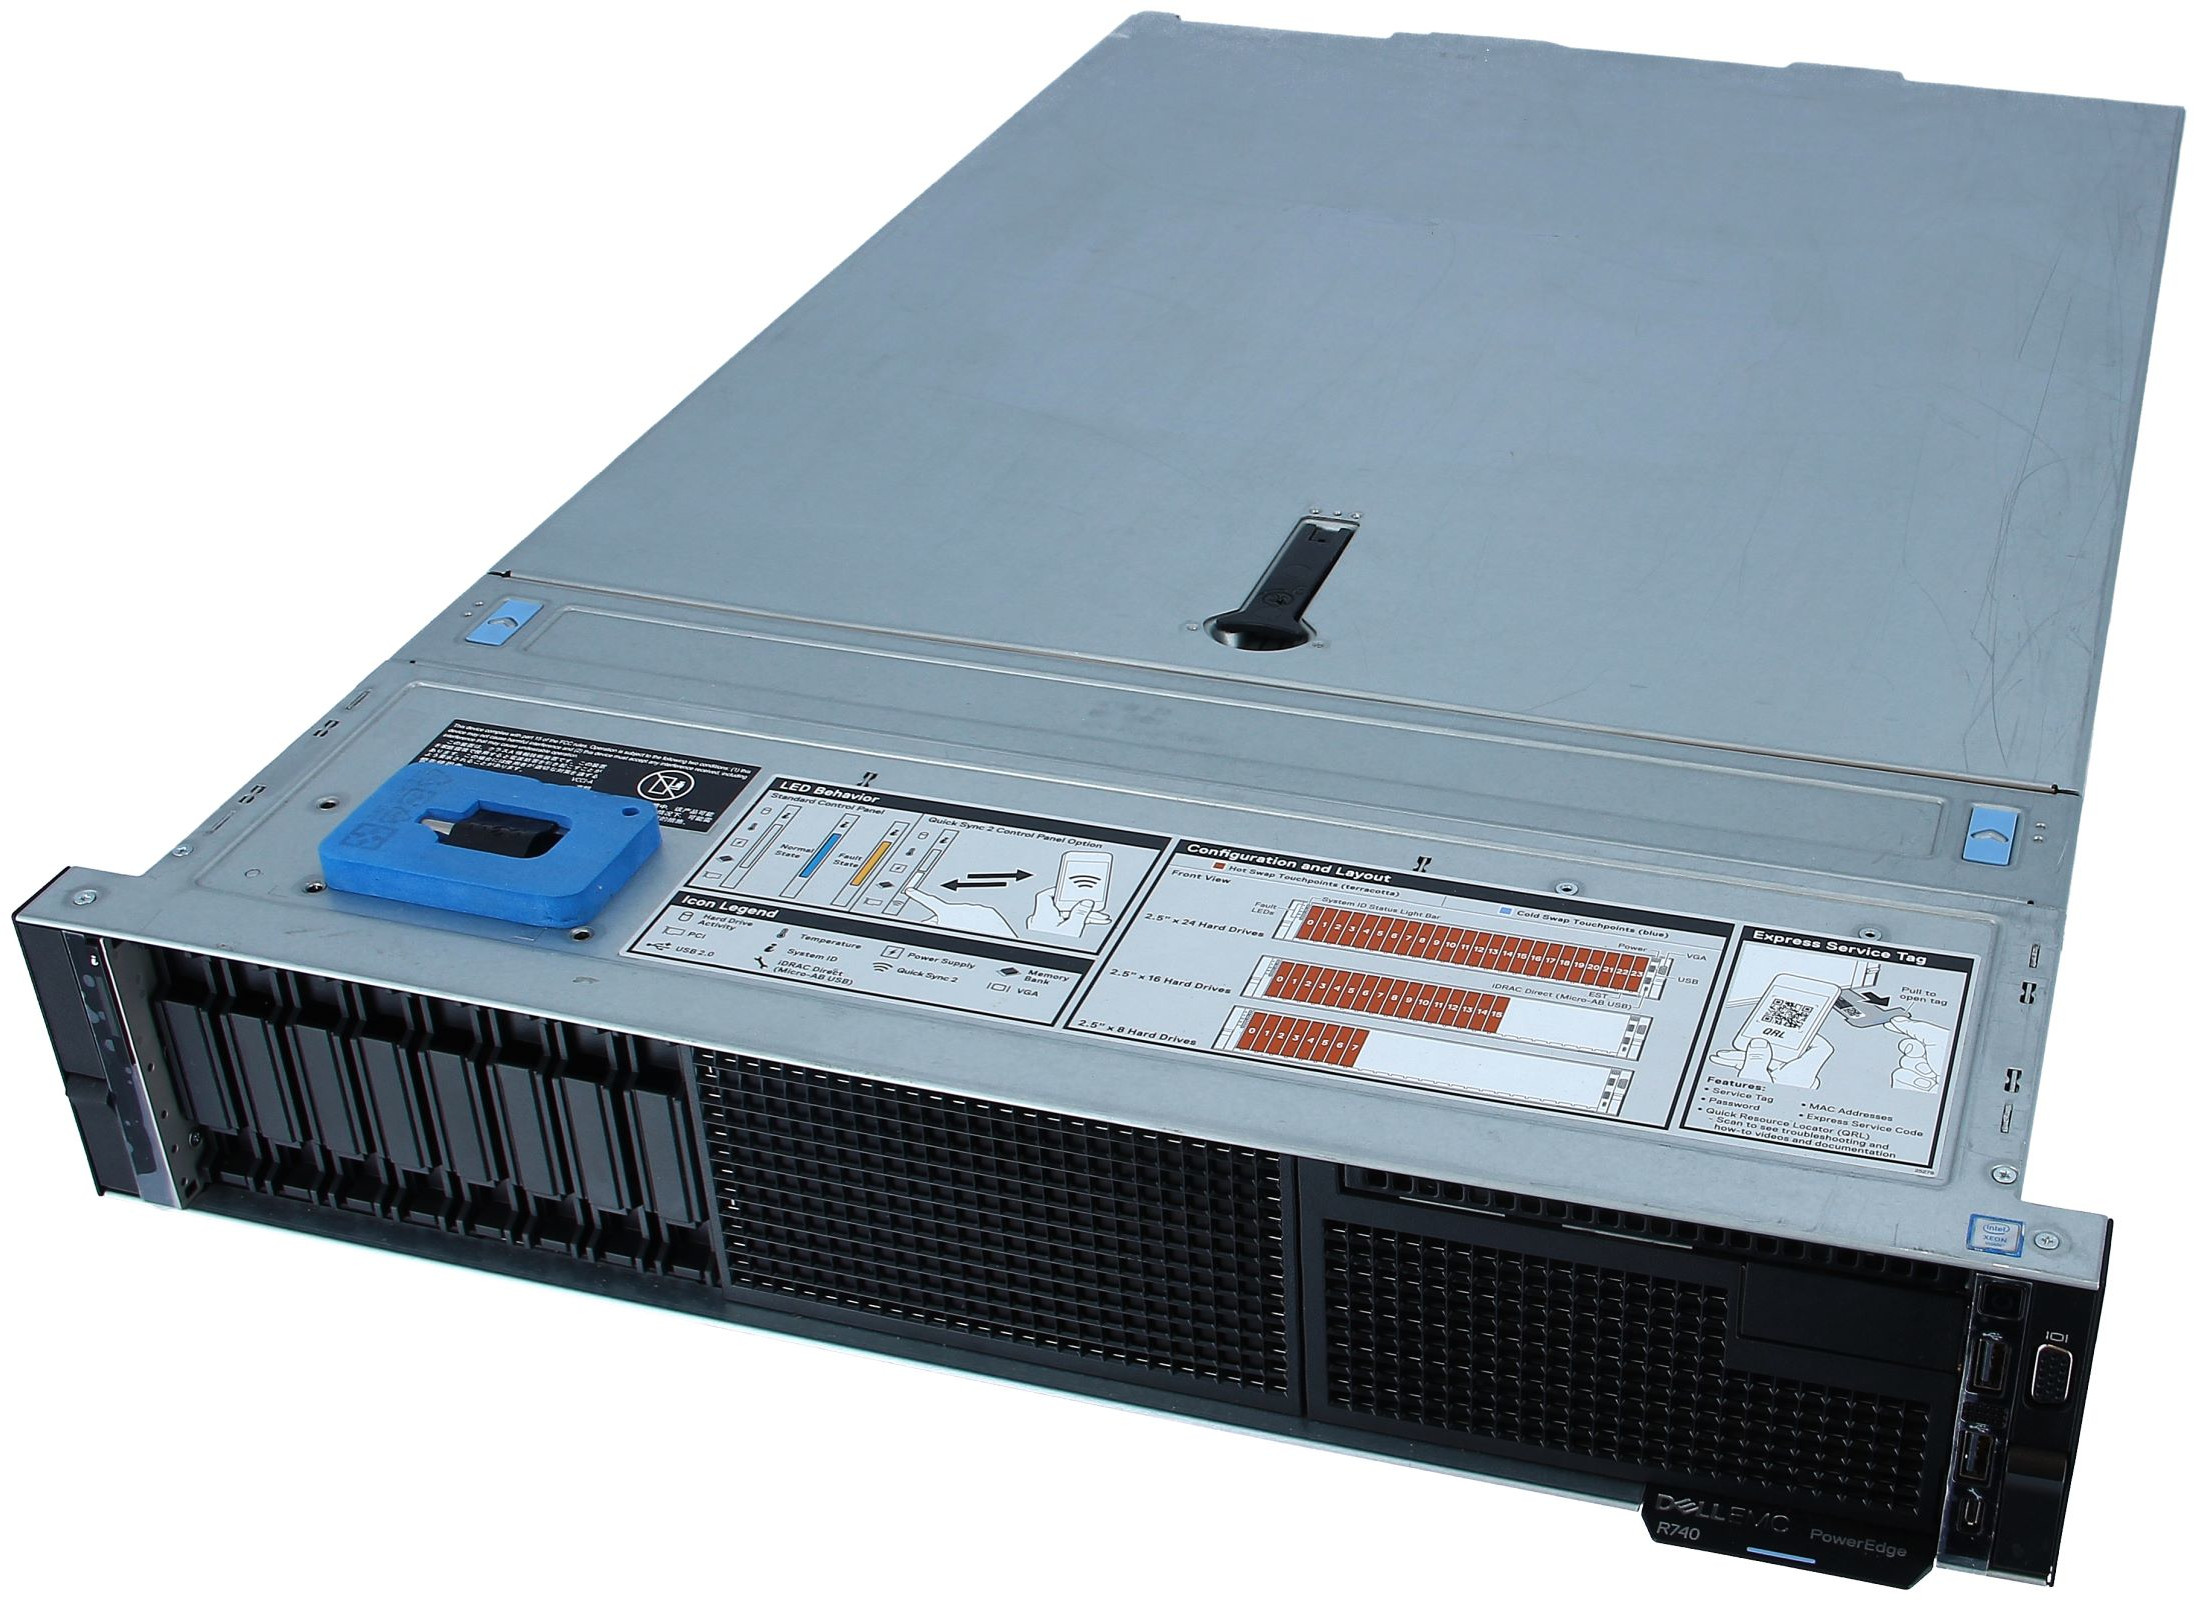
\includegraphics[width=3cm]{dell1}};
      \node[inner sep=2pt, draw] at ( 0, -2) (Pj) {$P_j$};
      \draw (Pj) -- (0, -2.5);
      \draw[fill=green] (-1, -2.5) rectangle (1, -7);

      \draw[fill=red]   (-1, -3) rectangle (1, -6);
      \draw[fill=yellow!50] (-0.9, -5) rectangle node {data} +(1.8, -1);
      \draw[thick] (1.2, -3) -- node[anchor=west] {\mintinline{C}{MPI_Recv}} (1.2, -6);
    \end{scope}

    \draw[ultra thick, ->] (1, -5) -- ++(1, 0) -- (5, -5.5) -- ++(1, 0);
  \end{tikzpicture}  
\end{frame}

%%%%%%%%%%%%%%%%%%%%%%%%%%%%%%%%%%%%%%%%%%%%%%%%%%%%%%%%%%%%%%%%%%%%%%%%%%%%%%%%%%%%%%%%%%%%%%%

\begin{frame}[fragile]
  \frametitle{More Point-to-Point Functions}

  \begin{exampleblock}{Receiving}
    \begin{center}
    \begin{tabular}{|c||c|}
    \hline
    Blocking     & \mintinline{C}{MPI_Recv}   \\
    \hline
    Non-blocking & \mintinline{C}{MPI_Irecv}  \\
    \hline
    \end{tabular}
  \end{center}
\end{exampleblock}

\pause
  
  \begin{alertblock}{Sending}
    \begin{center}
      \begin{tabular}{|c||c|c|c|}
    \hline
                 & Synchronous                 & Buffered                  & Standard \\
    \hline\hline
    Blocking     & \mintinline{C}{MPI_Ssend}   & \mintinline{C}{MPI_Bsend} & \mintinline{C}{MPI_Send}    \\
    \hline
    Non-blocking & \mintinline{C}{MPI_Issend}  & \mintinline{C}{MPI_Ibsend} & \mintinline{C}{MPI_Isend}  \\
    \hline
    \end{tabular}
    \end{center}
  \end{alertblock}

  \begin{itemize}
  \item I = ``Immediate''
  \item Non-blocking functions return as soon as possible
  \item Operation runs \alert{in the background}
    \begin{itemize}
    \item[$\Rightarrow$] Overlap communication with computation
    \end{itemize}
  \end{itemize}
  
\end{frame}

%%%%%%%%%%%%%%%%%%%%%%%%%%%%%%%%%%%%%%%%%%%%%%%%%%%%%%%%%%%%%%%%%%%%%%%%%%%%%%%%%%%%%%%%%%%%%

\begin{frame}[fragile=singleslide]
  \frametitle{Non-Blocking Receive}

  \begin{tikzpicture}[xscale=0.8]
    \path[use as bounding box] (-3, -6) rectangle (11, 0.5);
    \begin{scope}[xshift=0cm, yscale=1]
      \node at (0, -0.5) {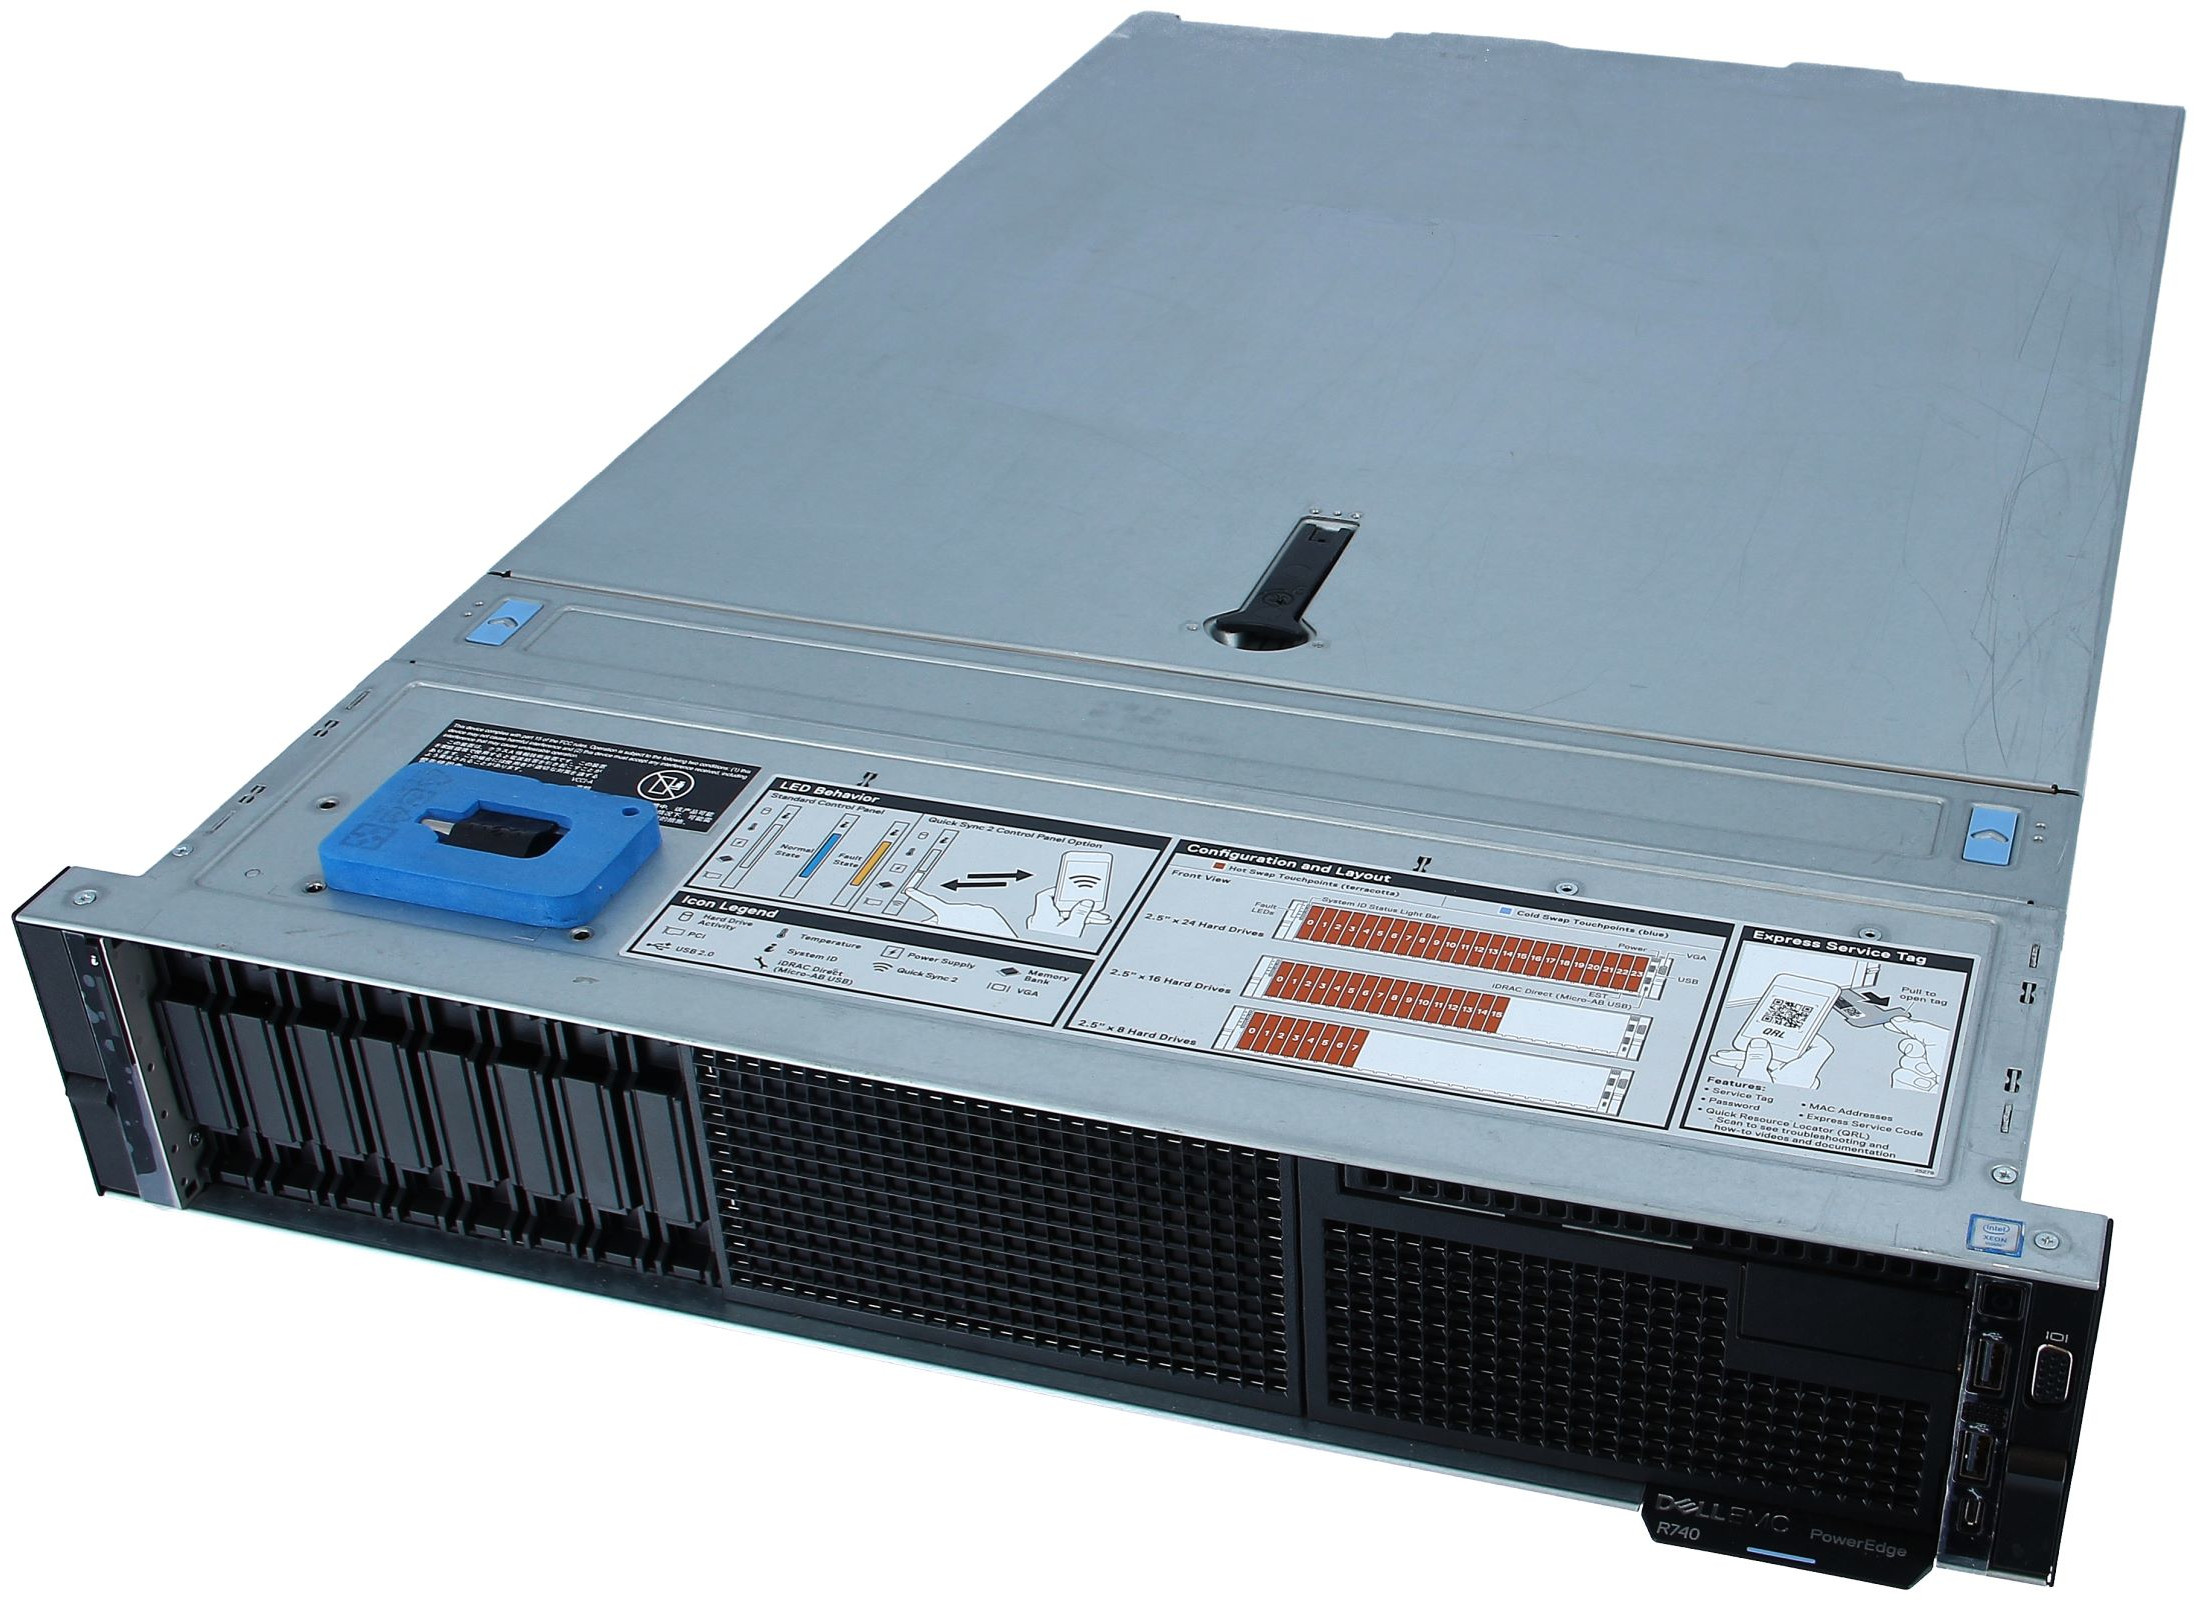
\includegraphics[width=3cm]{dell1}};
      \node[inner sep=2pt, draw] at ( 0, -2) (Pi) {$P_i$};
      \draw (Pi) -- (0, -2.5);
      \draw[fill=green] (-1, -2.5) rectangle (1, -7);
      
      \draw[fill=red]   (-1, -4.4) rectangle +(2, -1.1);
      \draw[fill=yellow!50] (-0.9, -4.5) rectangle node {data} +(1.8, -1);
      \draw[thick] (-1.2, -4.4) -- node[anchor=east] {\mintinline{C}{MPI_Send}} ++(0, -1.1);
    \end{scope}

    \begin{scope}[xshift=7cm]
      \node at (0, -0.5) {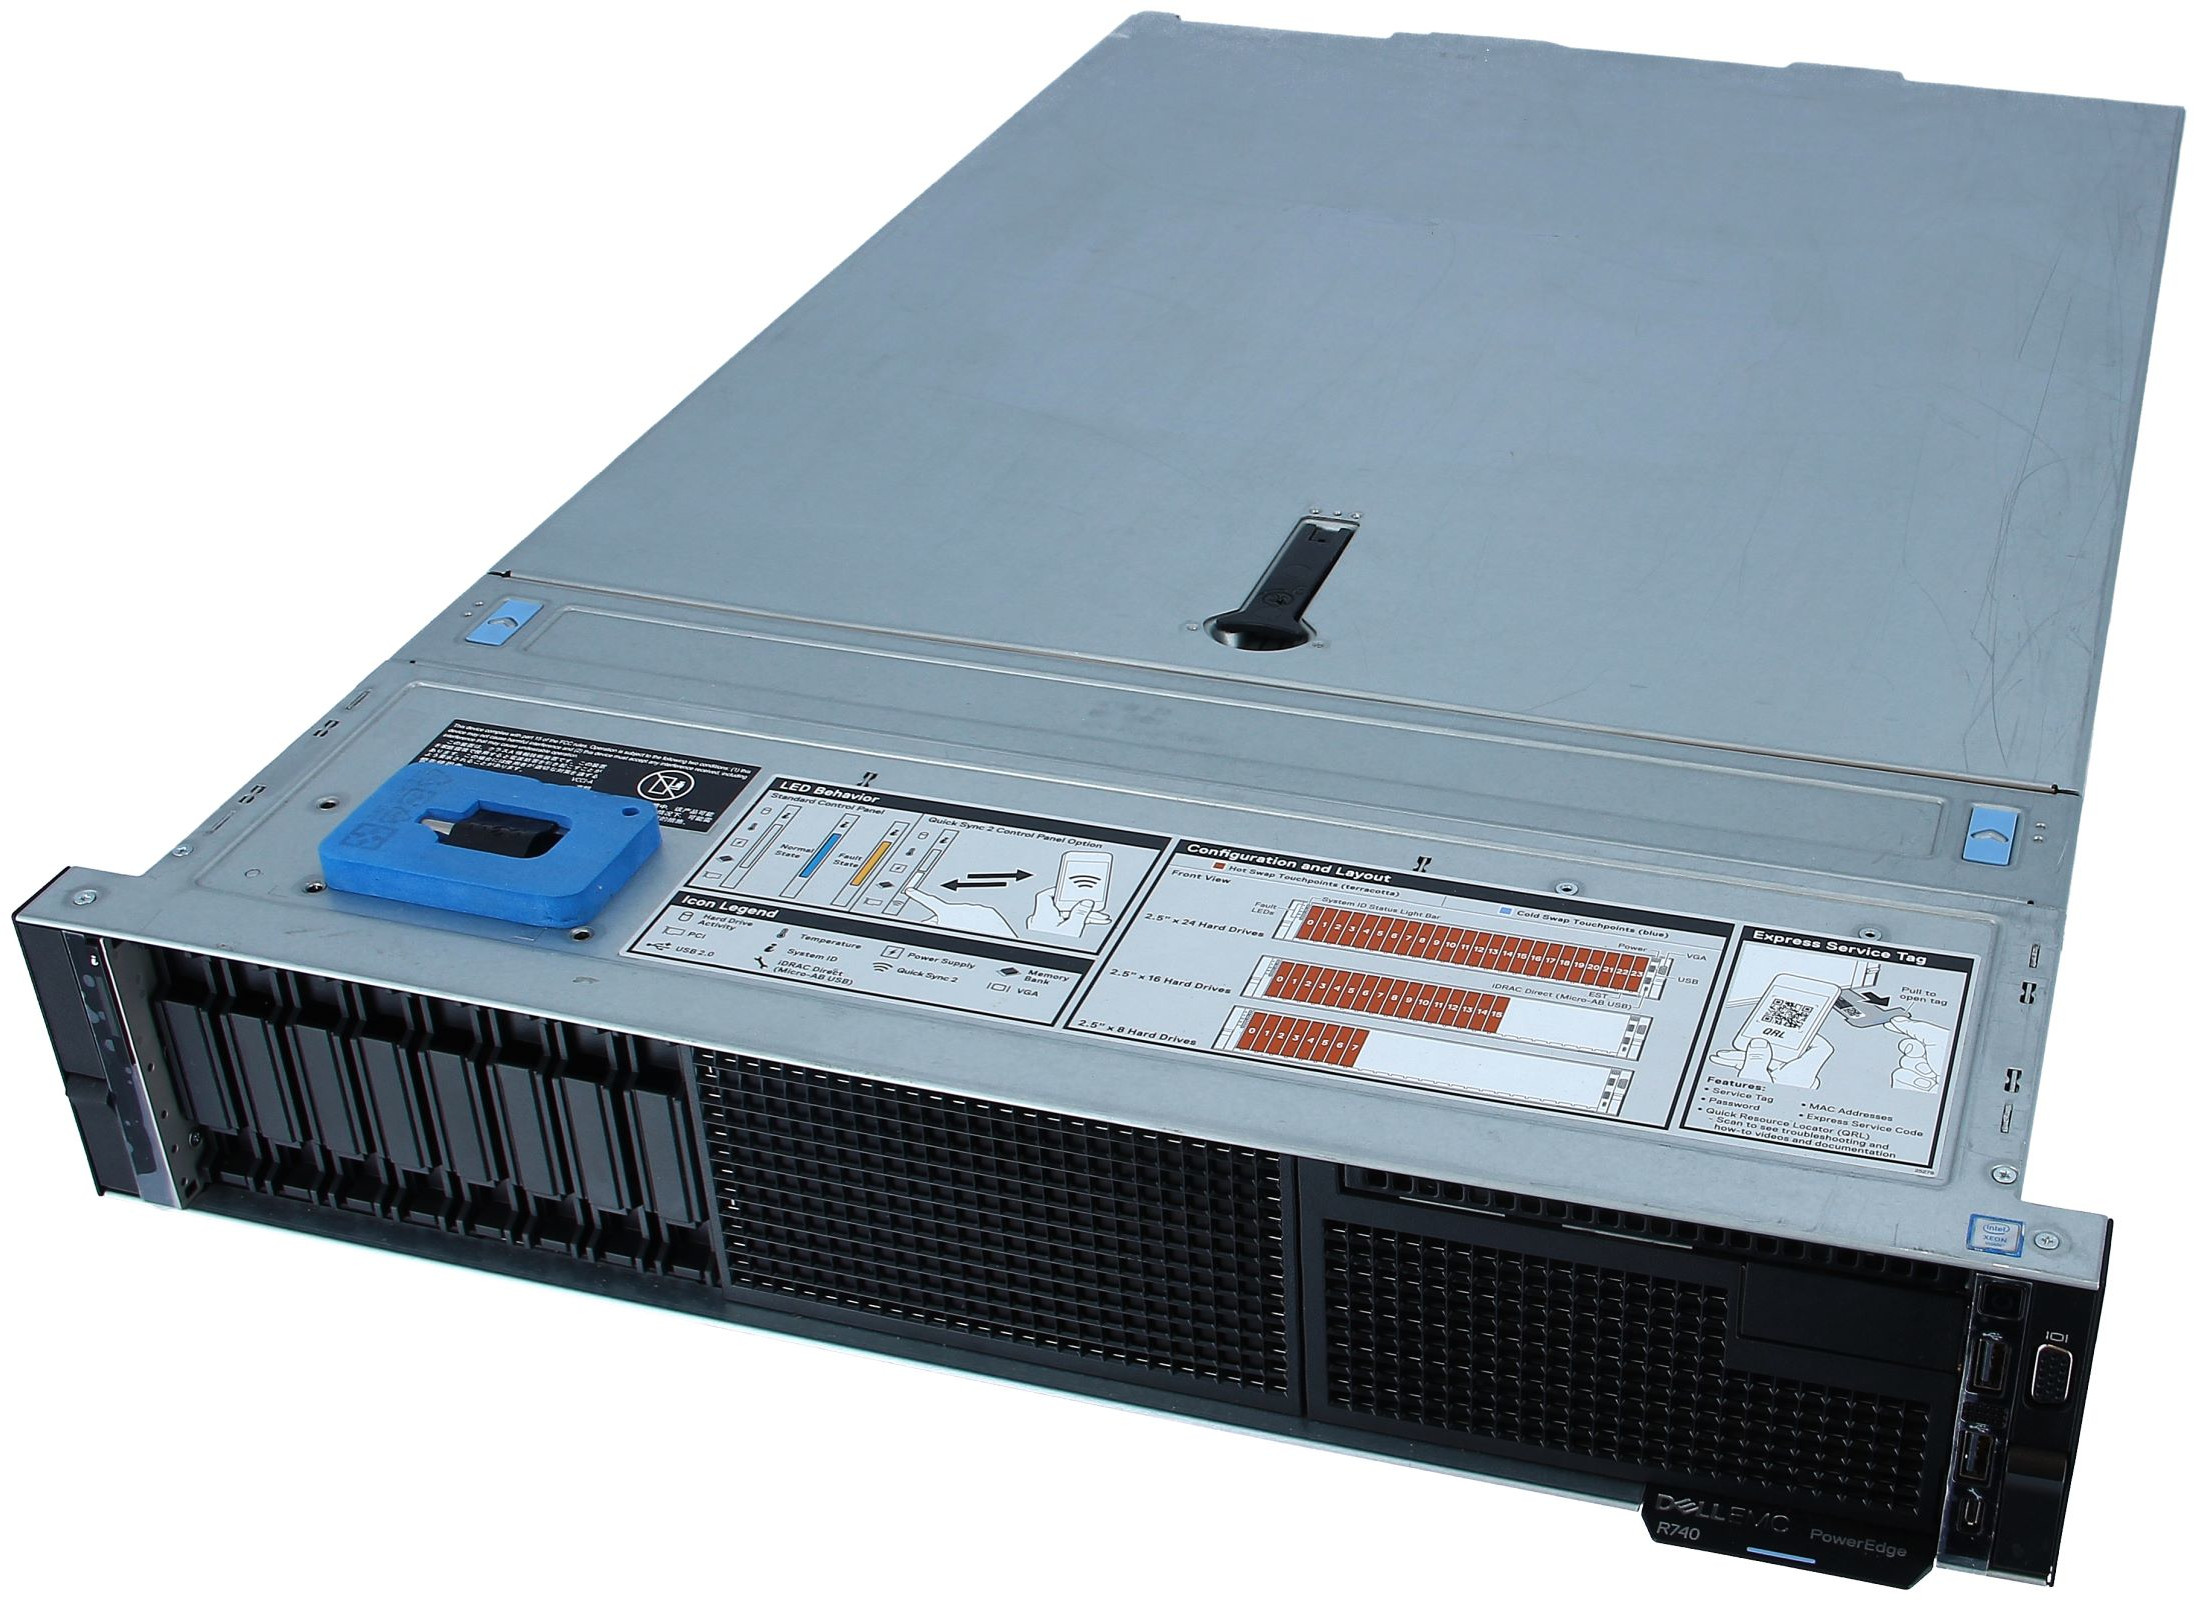
\includegraphics[width=3cm]{dell1}};
      \node[inner sep=2pt, draw] at ( 0, -2) (Pj) {$P_j$};
      \draw (Pj) -- (0, -2.5);
      \draw[fill=green] (-1, -2.5) rectangle (1, -7);

      \draw[fill=red]   (-1, -3) rectangle (1, -3.2);
      \draw[fill=yellow!50] (-0.9, -5) rectangle node {data} +(1.8, -1);
      \draw[thick] (1.2, -3) -- node[anchor=west] {\mintinline{C}{MPI_Irecv}} (1.2, -3.2);

      \draw[<-,blue,thick] (1, -6) -- +(0.5, 0) node[anchor=west] {Completed};

    \end{scope}

    \draw[ultra thick, ->] (1, -5) -- ++(1, 0) -- (5, -5.5) -- ++(1, 0);
  \end{tikzpicture}  
\end{frame}

%%%%%%%%%%%%%%%%%%%%%%%%%%%%%%%%%%%%%%%%%%%%%%%%%%%%%%%%%%%%%%%%%%%%%%%%%%%%%%%%%%%%%%%%%%%%%%%

\begin{frame}[fragile=singleslide]
  \frametitle{Blocking Synchronous Send}

  \begin{tikzpicture}[xscale=0.8]
    \path[use as bounding box] (-3, -6) rectangle (11, 0.5);
    \begin{scope}[xshift=0cm, yscale=1]
      \node at (0, -0.5) {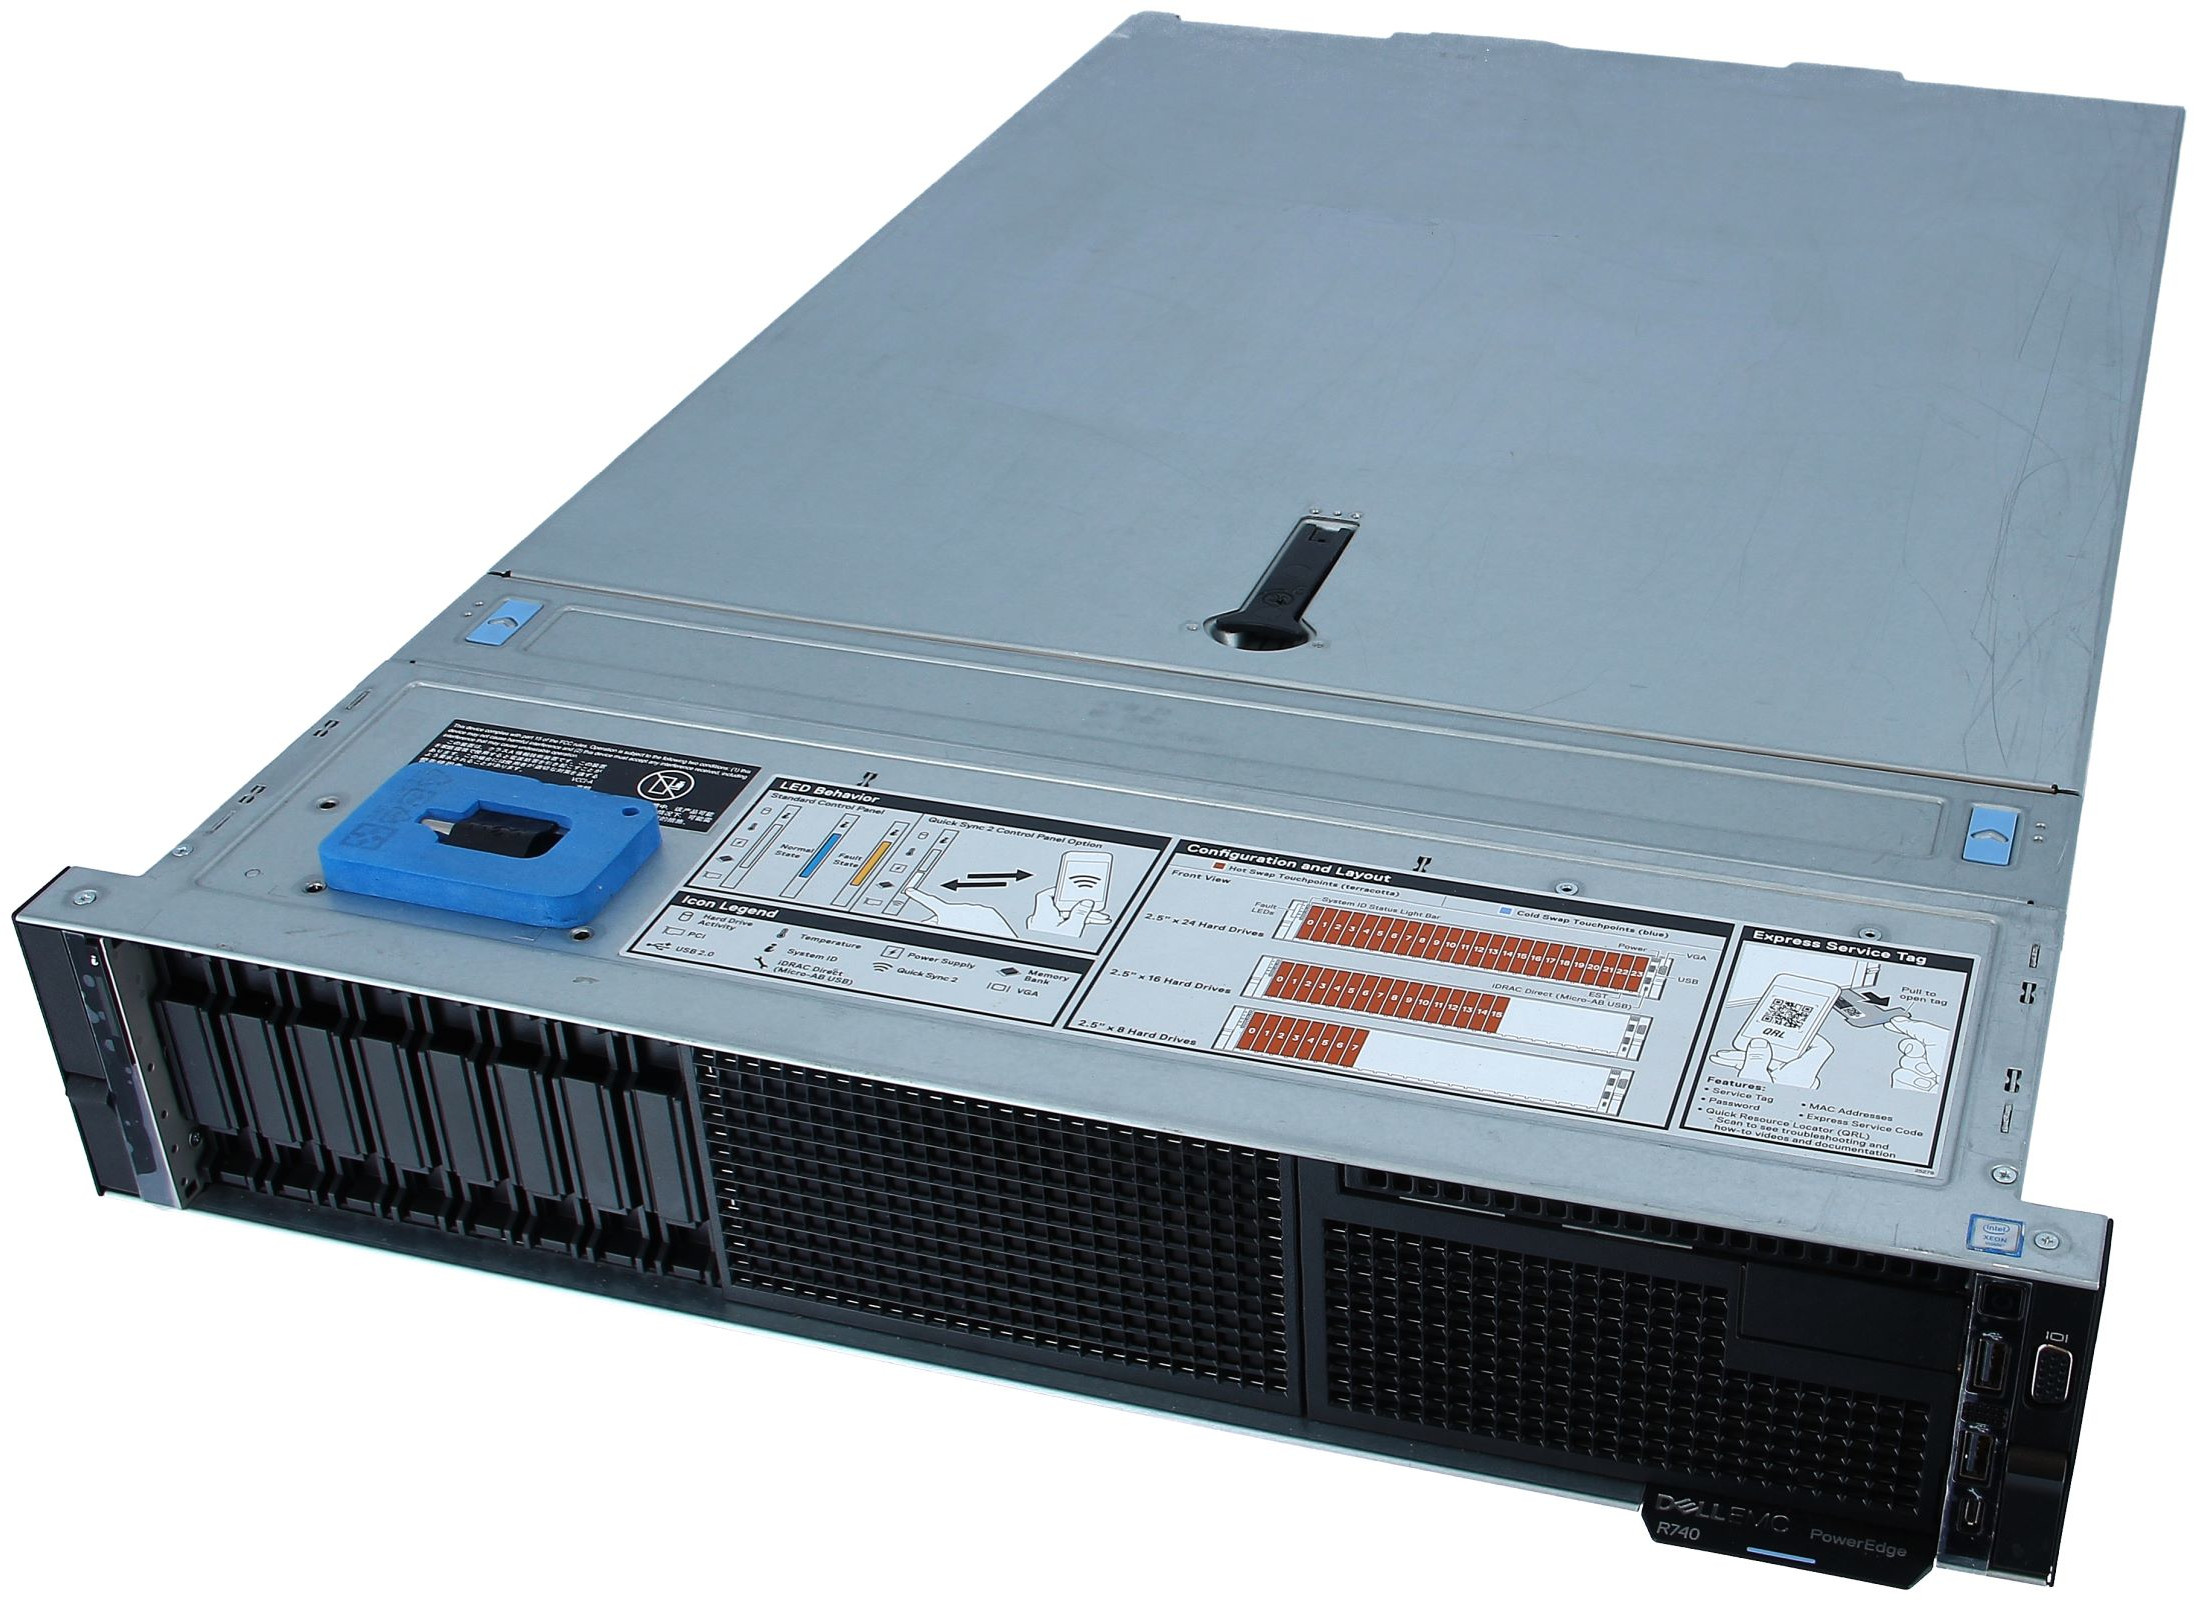
\includegraphics[width=3cm]{dell1}};
      \node[inner sep=2pt, draw] at ( 0, -2) (Pi) {$P_i$};
      \draw (Pi) -- (0, -2.5);
      \draw[fill=green] (-1, -2.5) rectangle (1, -7);
      
      \draw[fill=red]   (-1, -3) rectangle (1, -6);
      \draw[fill=yellow!50] (-0.9, -5) rectangle node {data} +(1.8, -1);
      \draw[thick] (-1.2, -3) -- node[anchor=east] {\mintinline{C}{MPI_Ssend}} ++(0, -3);
    \end{scope}

    \begin{scope}[xshift=7cm]
      \node at (0, -0.5) {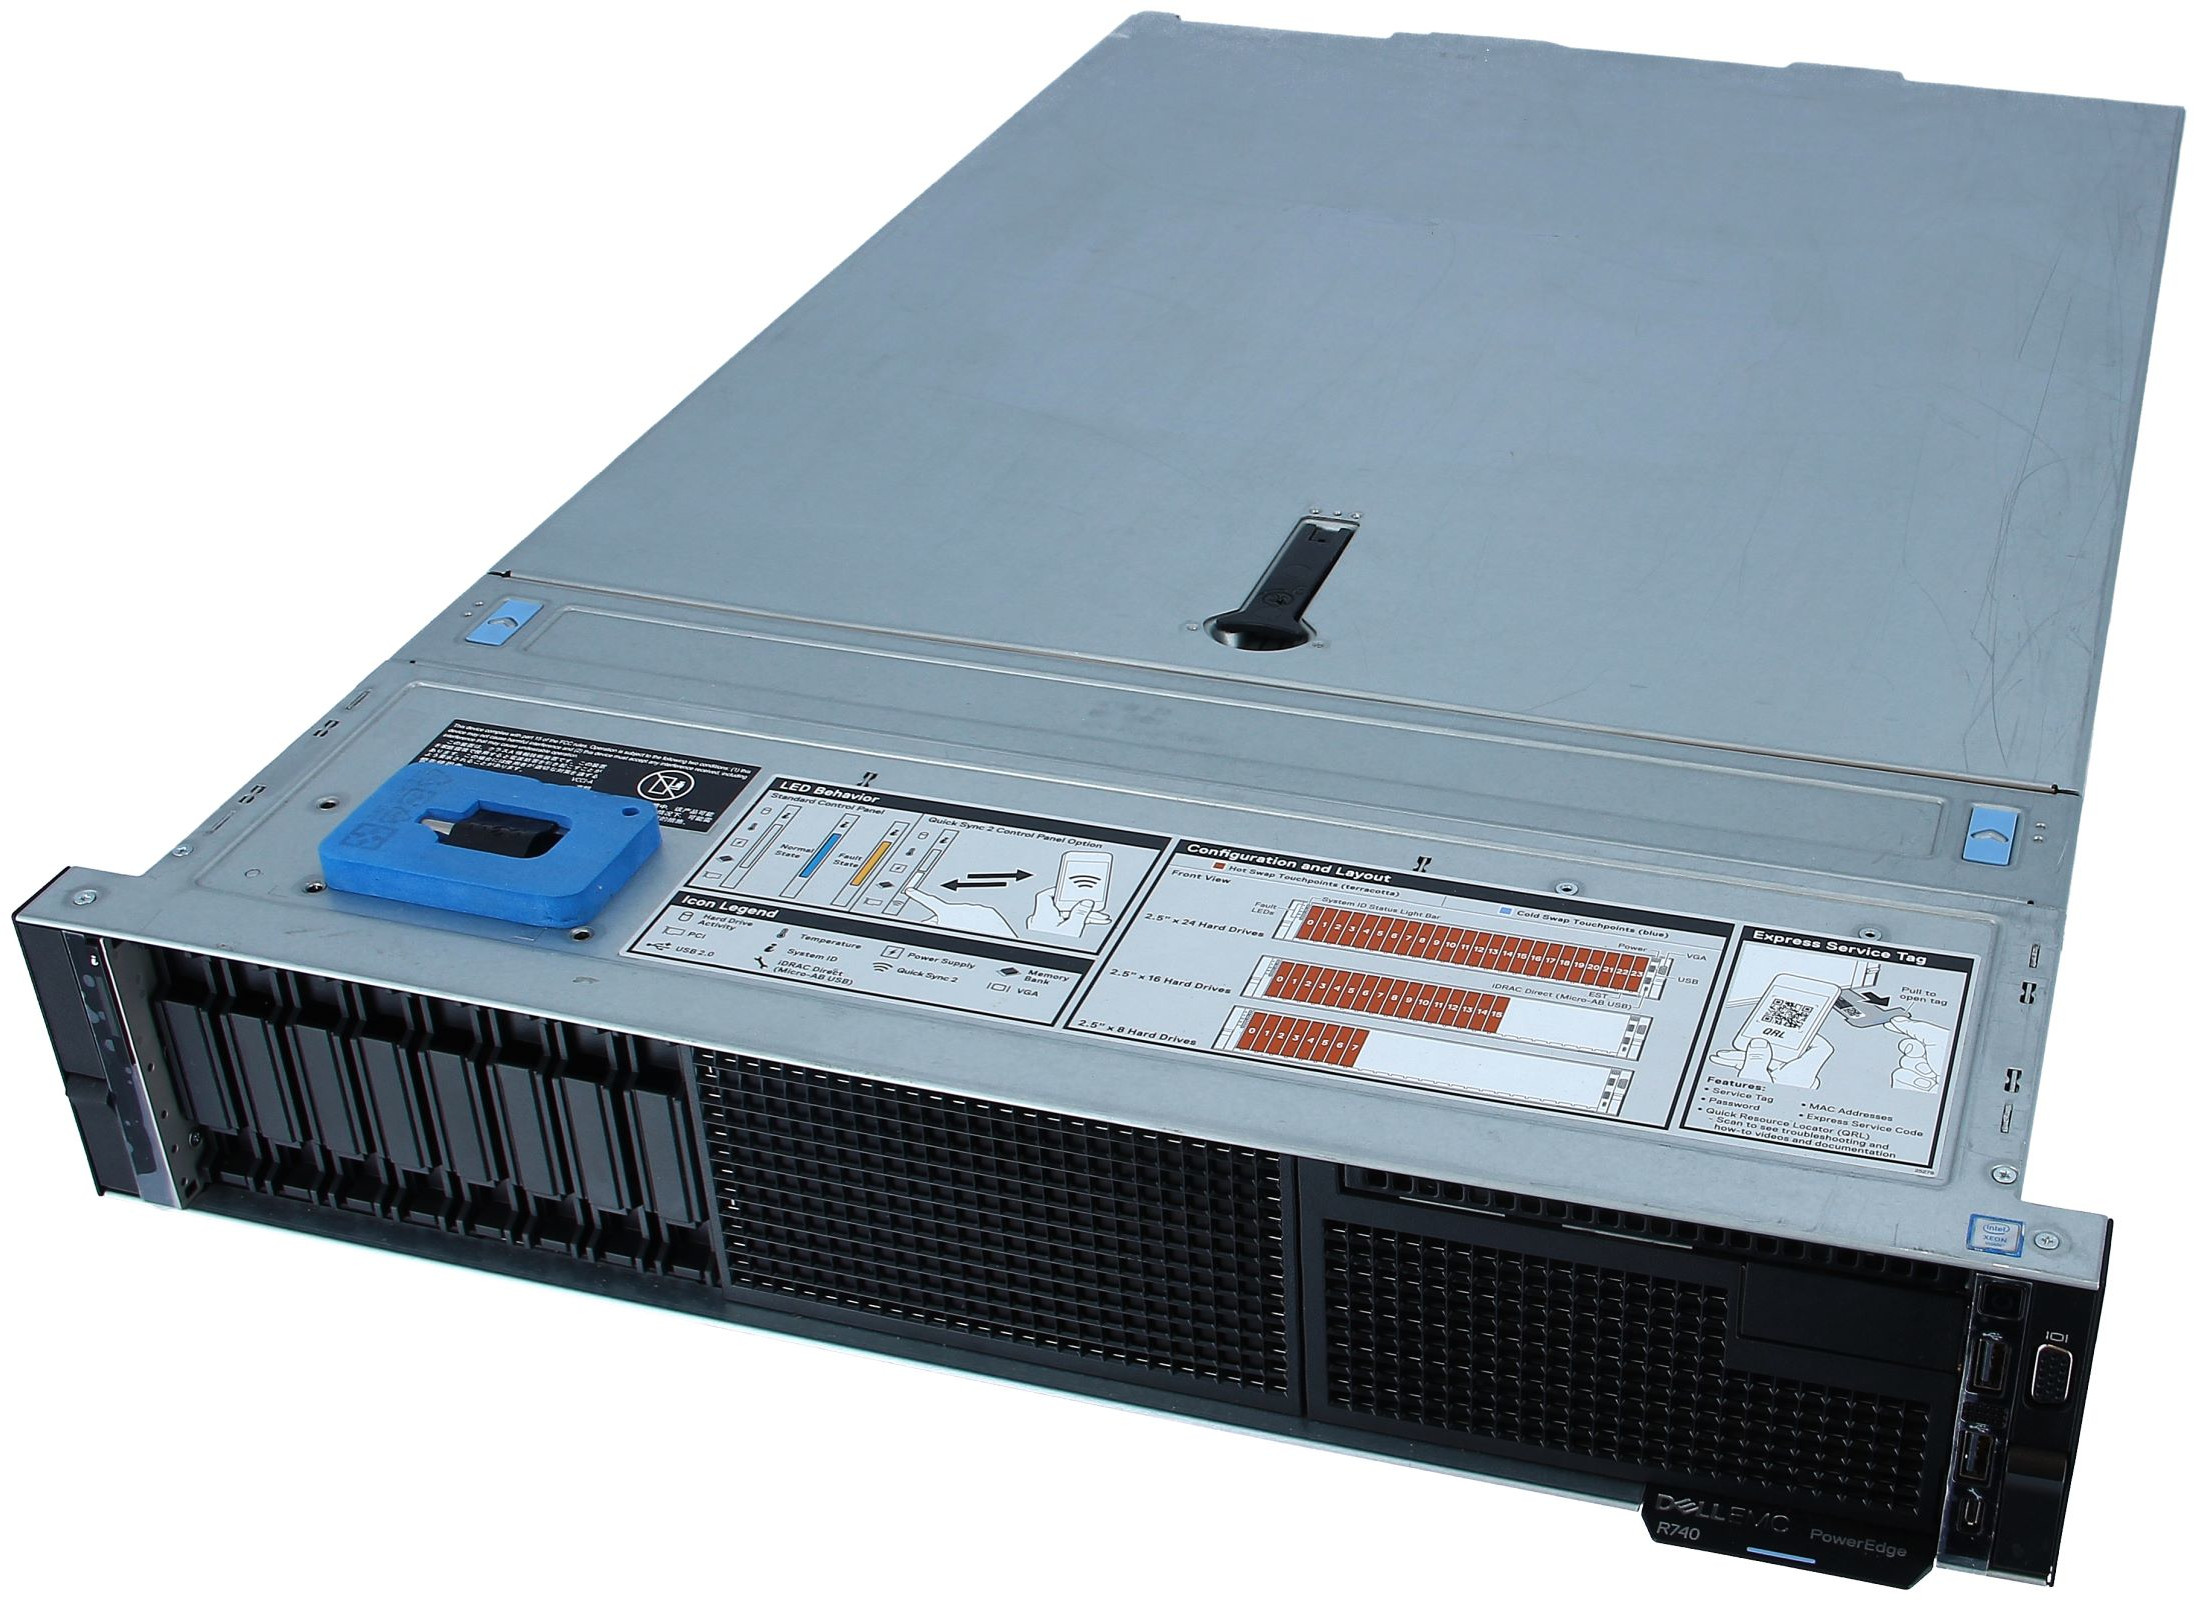
\includegraphics[width=3cm]{dell1}};
      \node[inner sep=2pt, draw] at ( 0, -2) (Pj) {$P_j$};
      \draw (Pj) -- (0, -2.5);
      \draw[fill=green] (-1, -2.5) rectangle (1, -7);

      \draw[fill=red]   (-1, -4.9) rectangle +(2, -1.5);
      \draw[fill=yellow!50] (-0.9, -5.4) rectangle node {data} +(1.8, -1);
      \draw[thick] (1.2, -4.9) -- node[anchor=west] {\mintinline{C}{MPI_Recv}} +(0, -1.5);

%      \draw[<-,blue,thick] (1, -6) -- +(0.5, 0) node[anchor=west] {Completed};

    \end{scope}

    \draw[ultra thick, ->] (1, -5.5) -- ++(1, 0) -- (5, -5.9) -- ++(1, 0);
    \draw[dashed] (1, -4.9) -- (6, -4.9);
  \end{tikzpicture}  
\end{frame}

%%%%%%%%%%%%%%%%%%%%%%%%%%%%%%%%%%%%%%%%%%%%%%%%%%%%%%%%%%%%%%%%%%%%%%%%%%%%%%%%%%%%%%%%%%%%%%%

\begin{frame}[fragile=singleslide]
  \frametitle{Blocking Buffered Send}

  \begin{tikzpicture}[xscale=0.8]
    \path[use as bounding box] (-3, -6) rectangle (11, 0.5);
    \begin{scope}[xshift=0cm, yscale=1]
      \node at (0, -0.5) {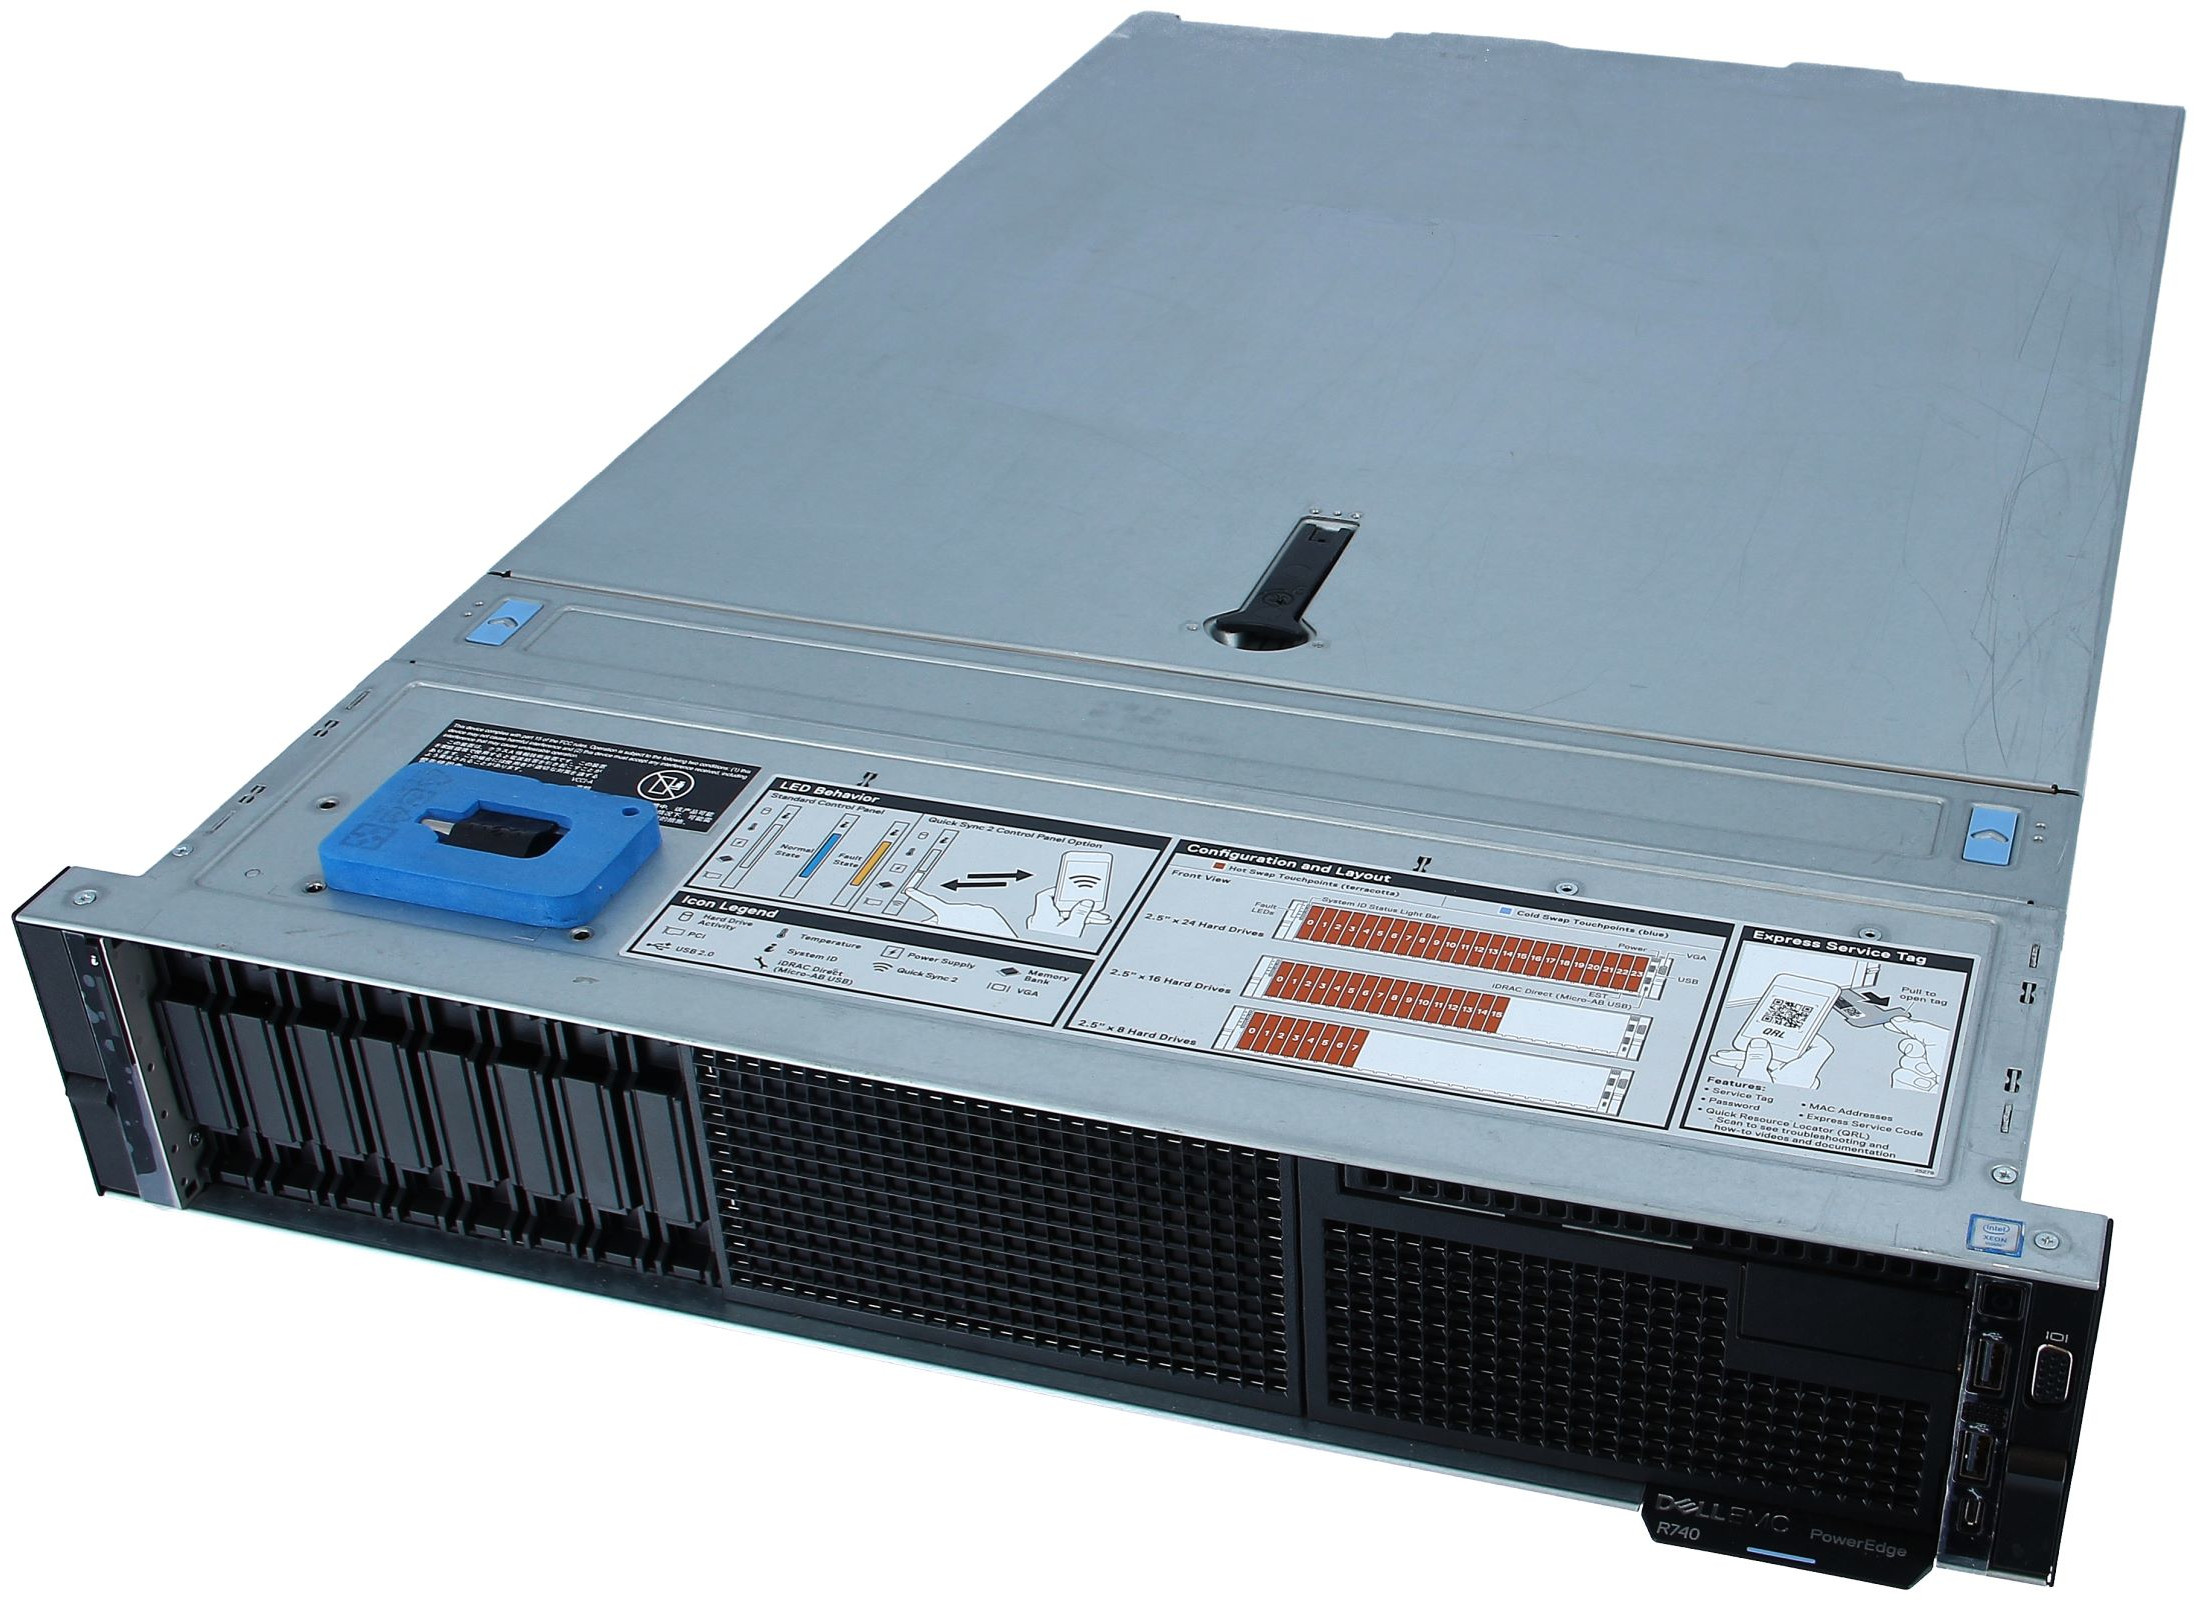
\includegraphics[width=3cm]{dell1}};
      \node[inner sep=2pt, draw] at ( 0, -2) (Pi) {$P_i$};
      \draw (Pi) -- (0, -2.5);
      \draw (Pi) -| (2.5, -4);

      \draw[fill=green] (-1, -2.5) rectangle (1, -7);
      \draw[fill=blue, semitransparent] (1.5, -4) rectangle +(2, -1.5);

      \draw[fill=red]   (-1, -3) rectangle (1, -4.1);
      \draw[fill=yellow!50] (-0.9, -3.1) rectangle node {data} +(1.8, -1);

      \draw[fill=yellow!50] (1.6, -4.1) rectangle node {data} +(1.8, -1);
      \node[white,anchor=south] at (2.5, -5.55) {buffer};
      
      \draw[thick] (-1.2, -3) -- node[anchor=east] {\mintinline{C}{MPI_Bsend}} ++(0, -1.1);
    \end{scope}

    \begin{scope}[xshift=7cm]
      \node at (0, -0.5) {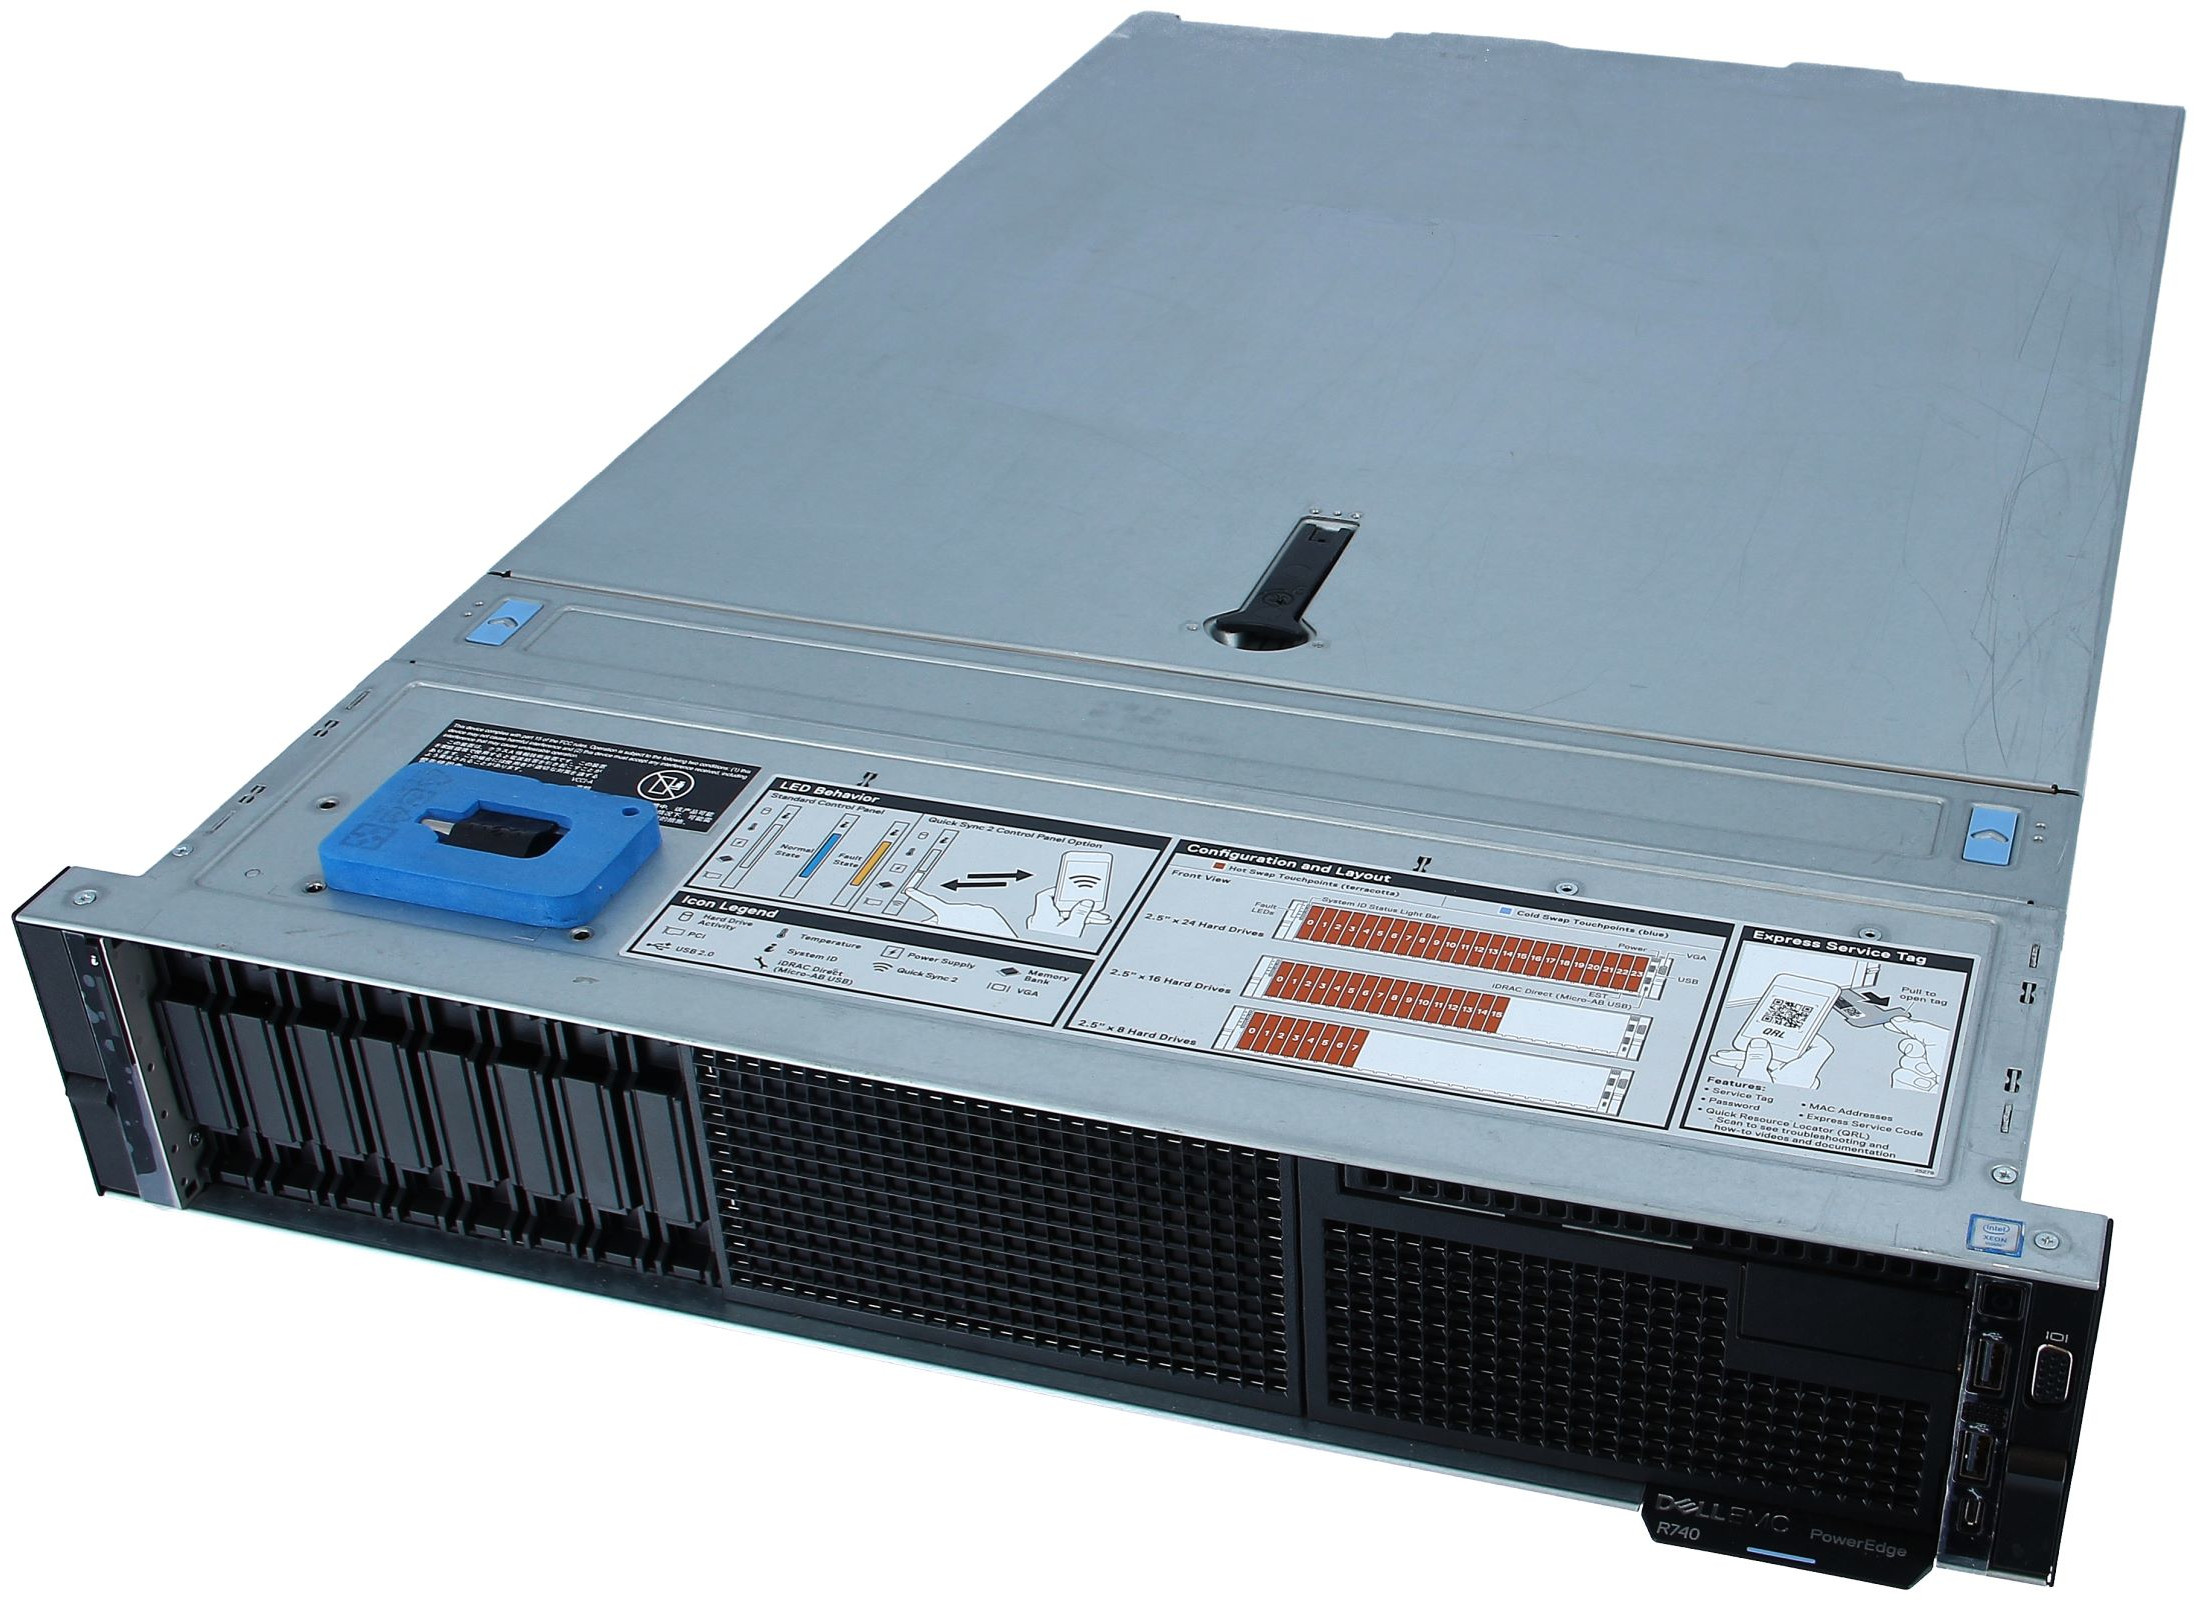
\includegraphics[width=3cm]{dell1}};
      \node[inner sep=2pt, draw] at ( 0, -2) (Pj) {$P_j$};
      \draw (Pj) -- (0, -2.5);
      \draw[fill=green] (-1, -2.5) rectangle (1, -7);

      \draw[fill=red]   (-1, -4.9) rectangle +(2, -1.1);
      \draw[fill=yellow!50] (-0.9, -5) rectangle node {data} +(1.8, -1);
      \draw[thick] (1.2, -4.9) -- node[anchor=west] {\mintinline{C}{MPI_Recv}} +(0, -1.1);

%      \draw[<-,blue,thick] (1, -6) -- +(0.5, 0) node[anchor=west] {Completed};

    \end{scope}

    \draw[ultra thick, ->] (1, -3.5) -| (2, -4);
    \draw[ultra thick, ->] (3.5, -4.6) -- ++(1, 0) -- (5, -5.5) -- ++(1, 0);
  \end{tikzpicture}  
\end{frame}

%%%%%%%%%%%%%%%%%%%%%%%%%%%%%%%%%%%%%%%%%%%%%%%%%%%%%%%%%%%%%%%%%%%%%%%%%%%%%%%%%%%%%%%%%%%%%

\begin{frame}[fragile=singleslide]
  \frametitle{Non-Blocking Synchronous Send}

  \begin{tikzpicture}[xscale=0.8]
    \path[use as bounding box] (-3, -6) rectangle (11, 0.5);
    \begin{scope}[xshift=0cm, yscale=1]
      \node at (0, -0.5) {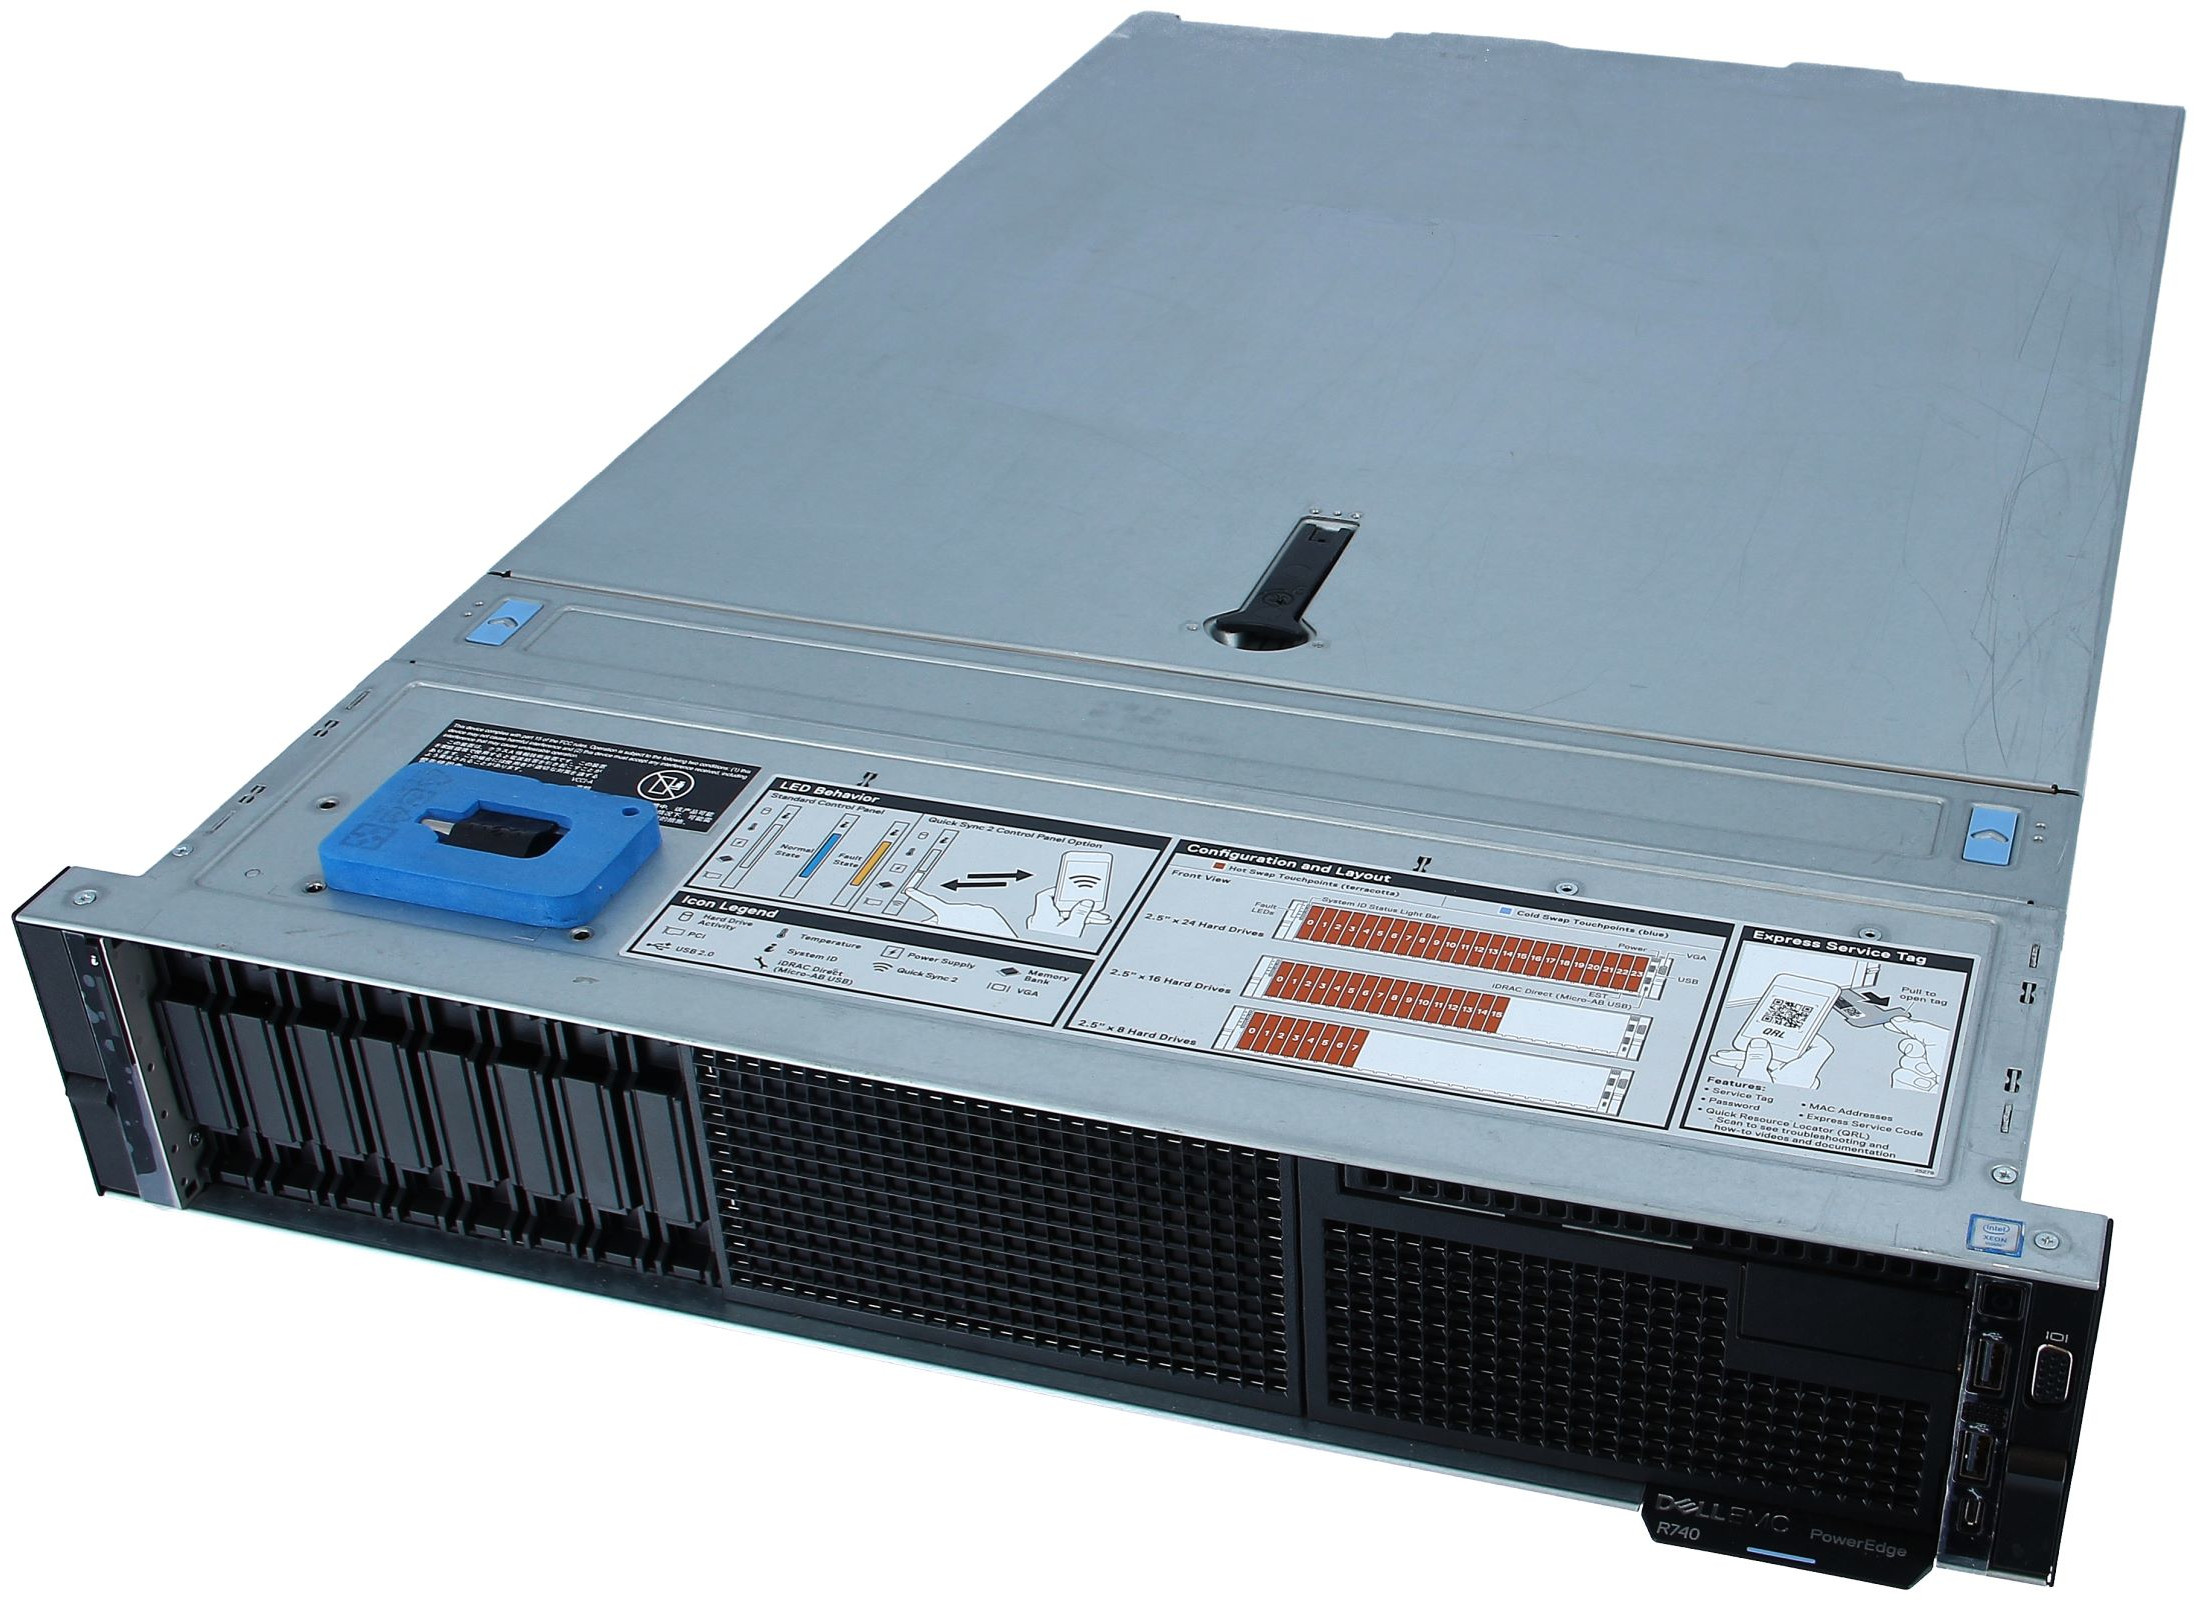
\includegraphics[width=3cm]{dell1}};
      \node[inner sep=2pt, draw] at ( 0, -2) (Pi) {$P_i$};
      \draw (Pi) -- (0, -2.5);
      \draw[fill=green] (-1, -2.5) rectangle (1, -7);
      
      \draw[fill=red]   (-1, -3) rectangle (1, -3.2);
      \draw[fill=yellow!50] (-0.9, -5) rectangle node {data} +(1.8, -1);
      \draw[thick] (-1.2, -3) -- node[anchor=east] {\mintinline{C}{MPI_Issend}} ++(0, -0.2);

      \draw[<-,blue,thick] (-1, -6) -- +(-0.5, 0) node[anchor=east] {Completed};
    \end{scope}

    \begin{scope}[xshift=7cm]
      \node at (0, -0.5) {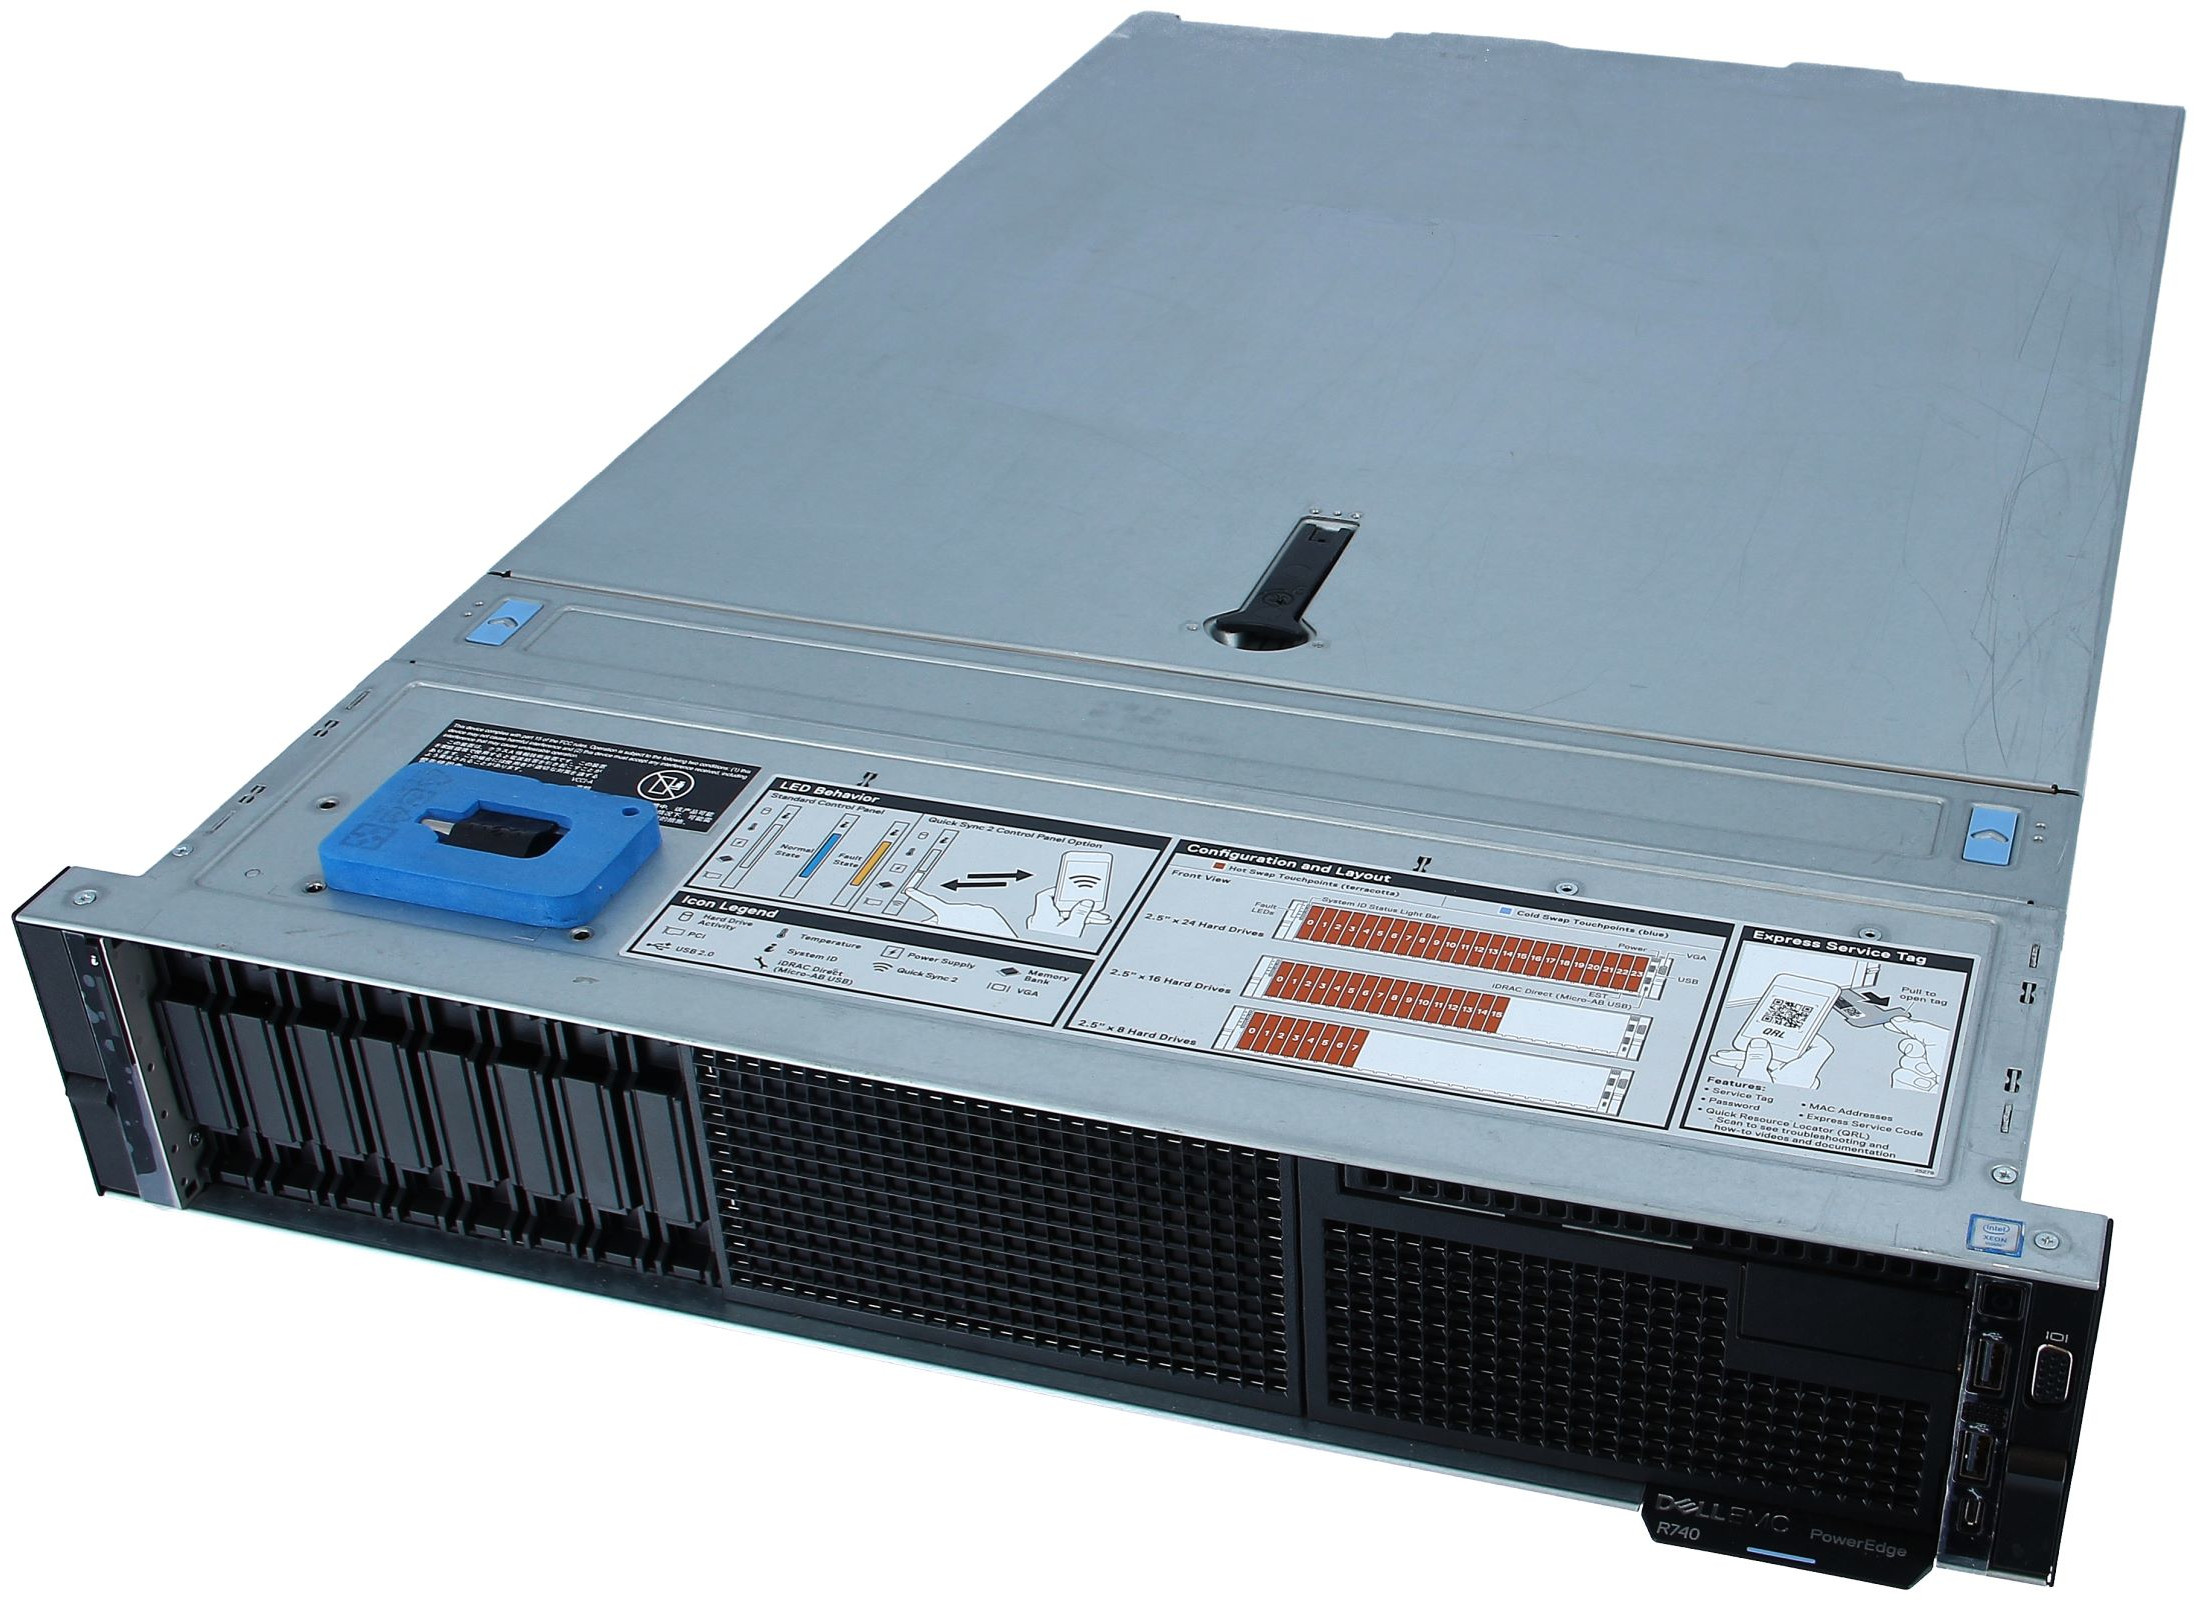
\includegraphics[width=3cm]{dell1}};
      \node[inner sep=2pt, draw] at ( 0, -2) (Pj) {$P_j$};
      \draw (Pj) -- (0, -2.5);
      \draw[fill=green] (-1, -2.5) rectangle (1, -7);

      \draw[fill=red]   (-1, -4.9) rectangle +(2, -1.5);
      \draw[fill=yellow!50] (-0.9, -5.4) rectangle node {data} +(1.8, -1);
      \draw[thick] (1.2, -4.9) -- node[anchor=west] {\mintinline{C}{MPI_Recv}} +(0, -1.5);
    \end{scope}

    \draw[ultra thick, ->] (1, -5.5) -- ++(1, 0) -- (5, -5.9) -- ++(1, 0);
    \draw[dashed] (1, -4.9) -- (6, -4.9);
  \end{tikzpicture}  
\end{frame}

%%%%%%%%%%%%%%%%%%%%%%%%%%%%%%%%%%%%%%%%%%%%%%%%%%%%%%%%%%%%%%%%%%%%%%%%%%%%%%%%%%%%%%%%%%%%%%%

\begin{frame}[fragile=singleslide]
  \frametitle{Non-Blocking Buffered Send}

  \begin{tikzpicture}[xscale=0.8]
    \path[use as bounding box] (-3, -6) rectangle (11, 0.5);
    \begin{scope}[xshift=0cm, yscale=1]
      \node at (0, -0.5) {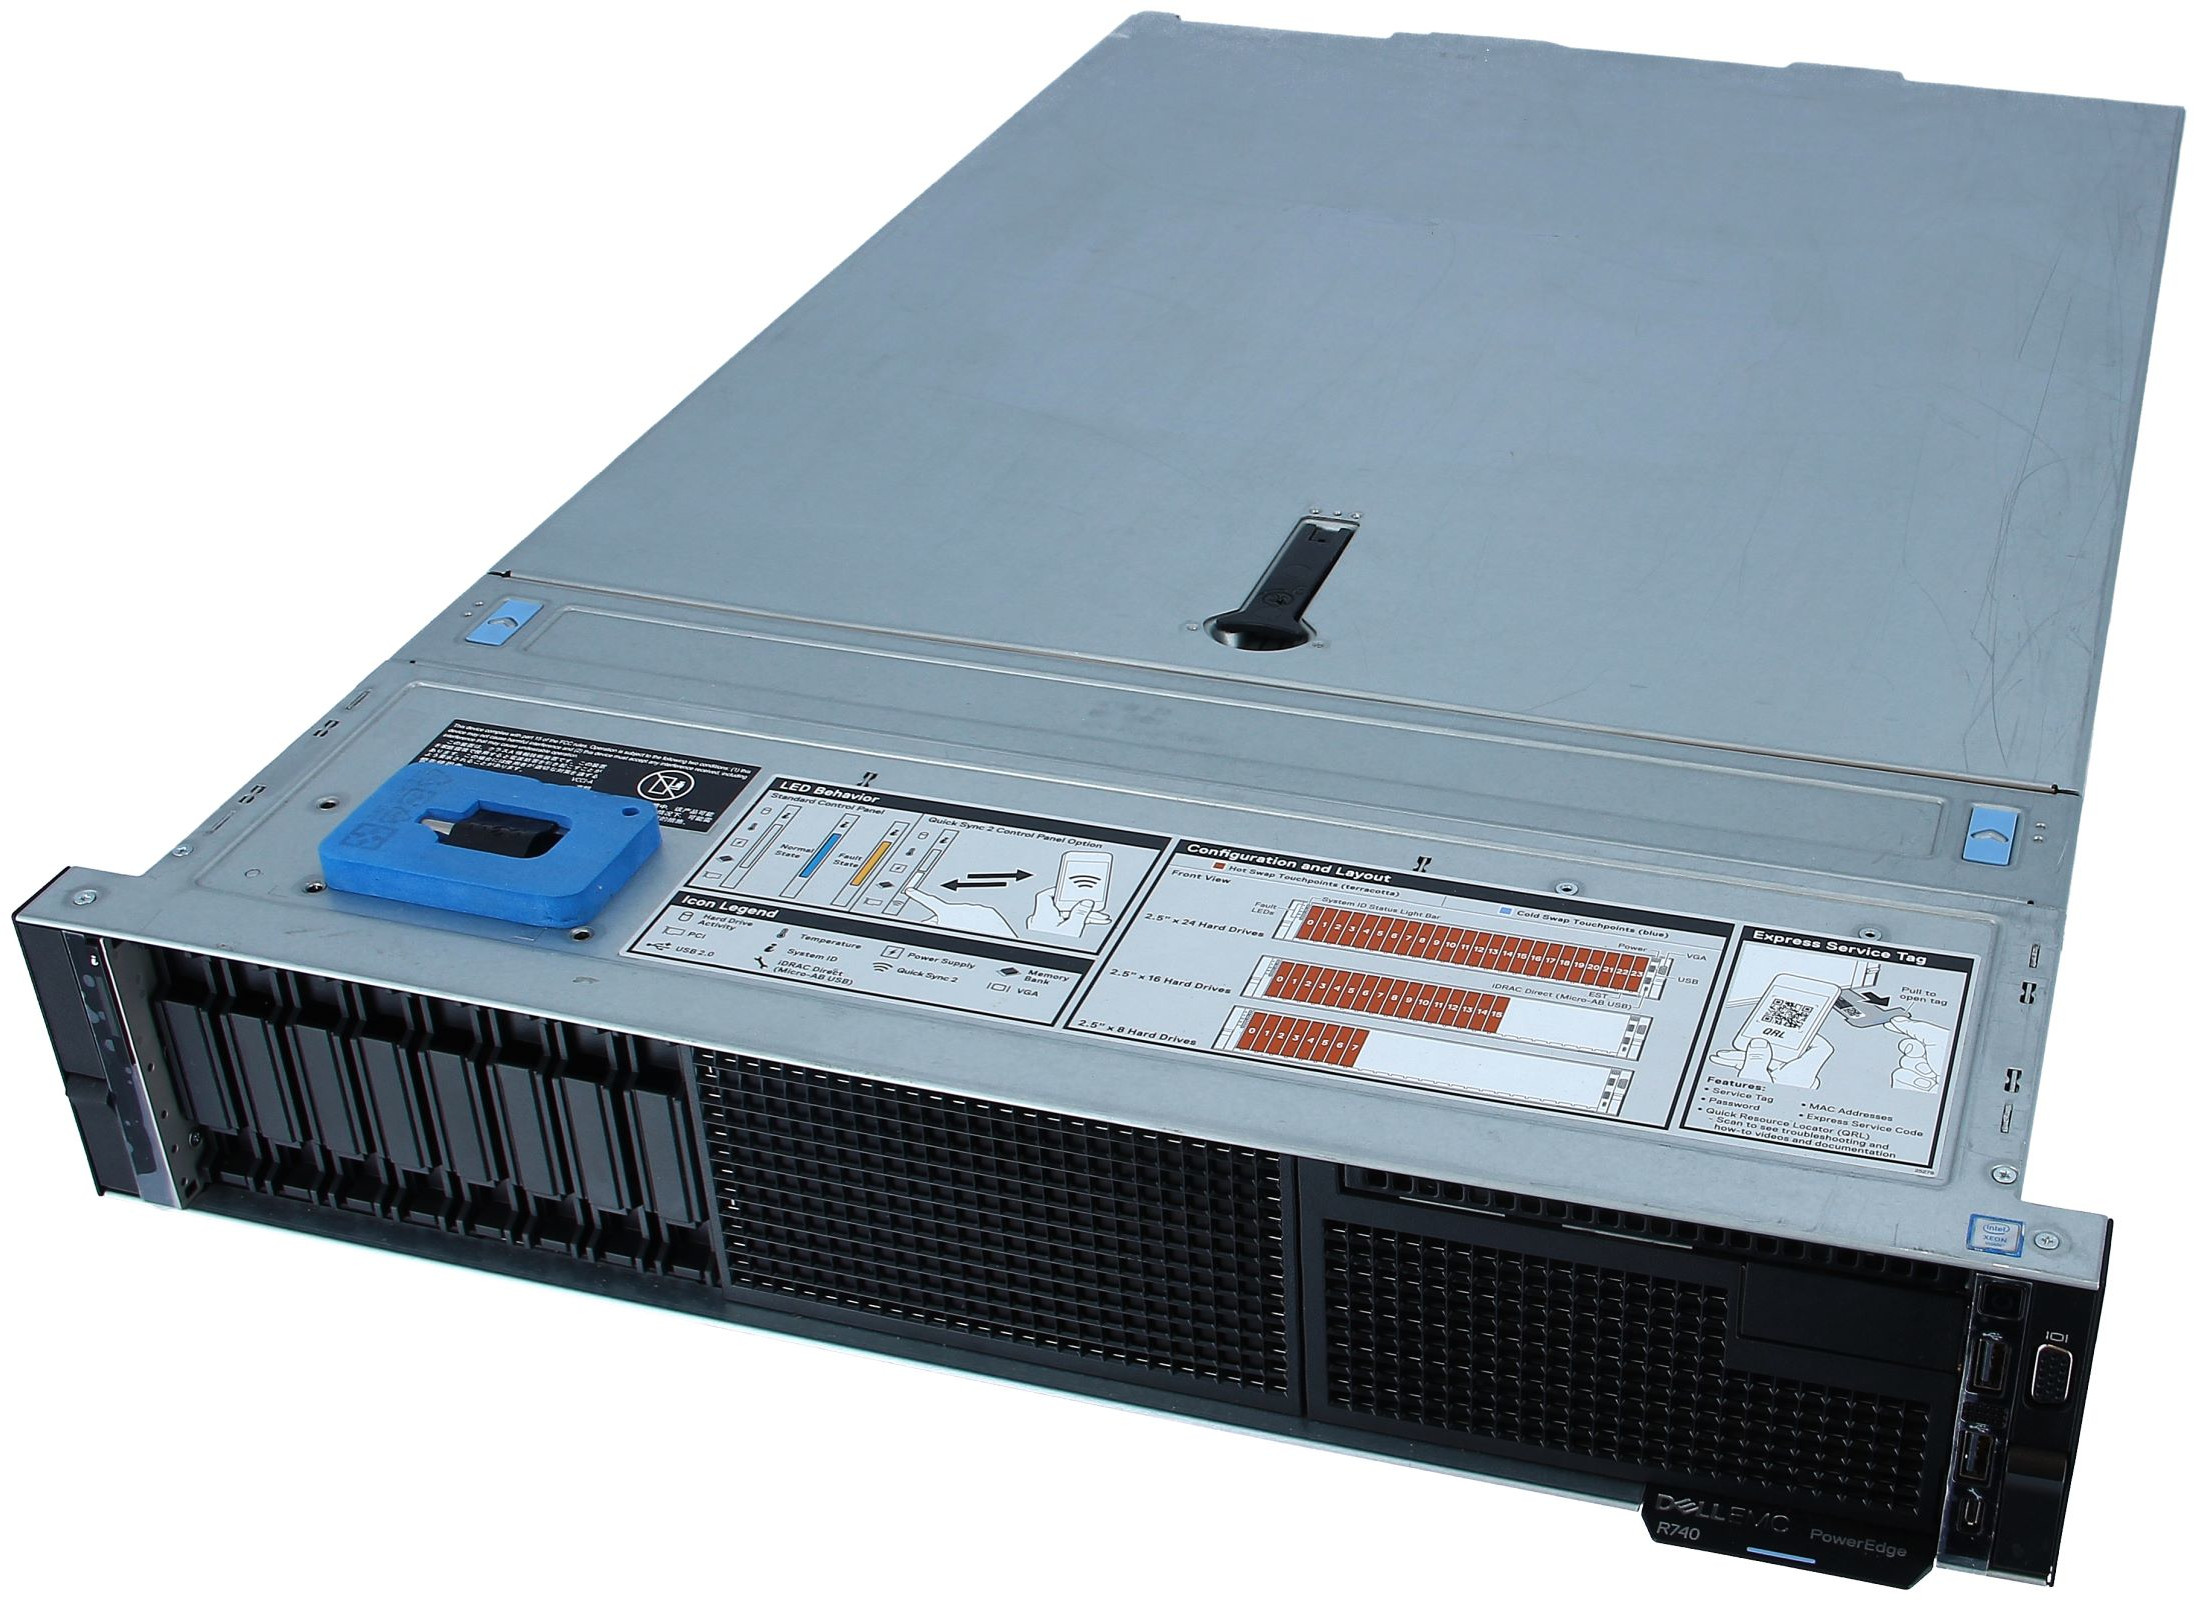
\includegraphics[width=3cm]{dell1}};
      \node[inner sep=2pt, draw] at ( 0, -2) (Pi) {$P_i$};
      \draw (Pi) -- (0, -2.5);
      \draw (Pi) -| (2.5, -4);

      \draw[fill=green] (-1, -2.5) rectangle (1, -7);
      \draw[fill=blue, semitransparent] (1.5, -4) rectangle +(2, -1.5);

      \draw[fill=red]   (-1, -3) rectangle (1, -3.2);
      \draw[fill=yellow!50] (-0.9, -3.1) rectangle node {data} +(1.8, -1);

      \draw[fill=yellow!50] (1.6, -4.1) rectangle node {data} +(1.8, -1);
      \node[white,anchor=south] at (2.5, -5.55) {buffer};
      
      \draw[thick] (-1.2, -3) -- node[anchor=east] {\mintinline{C}{MPI_Ibsend}} ++(0, -0.2);
      \draw[<-,blue,thick] (-1, -4.1) -- +(-0.5, 0) node[anchor=east] {Completed};
    \end{scope}

    \begin{scope}[xshift=7cm]
      \node at (0, -0.5) {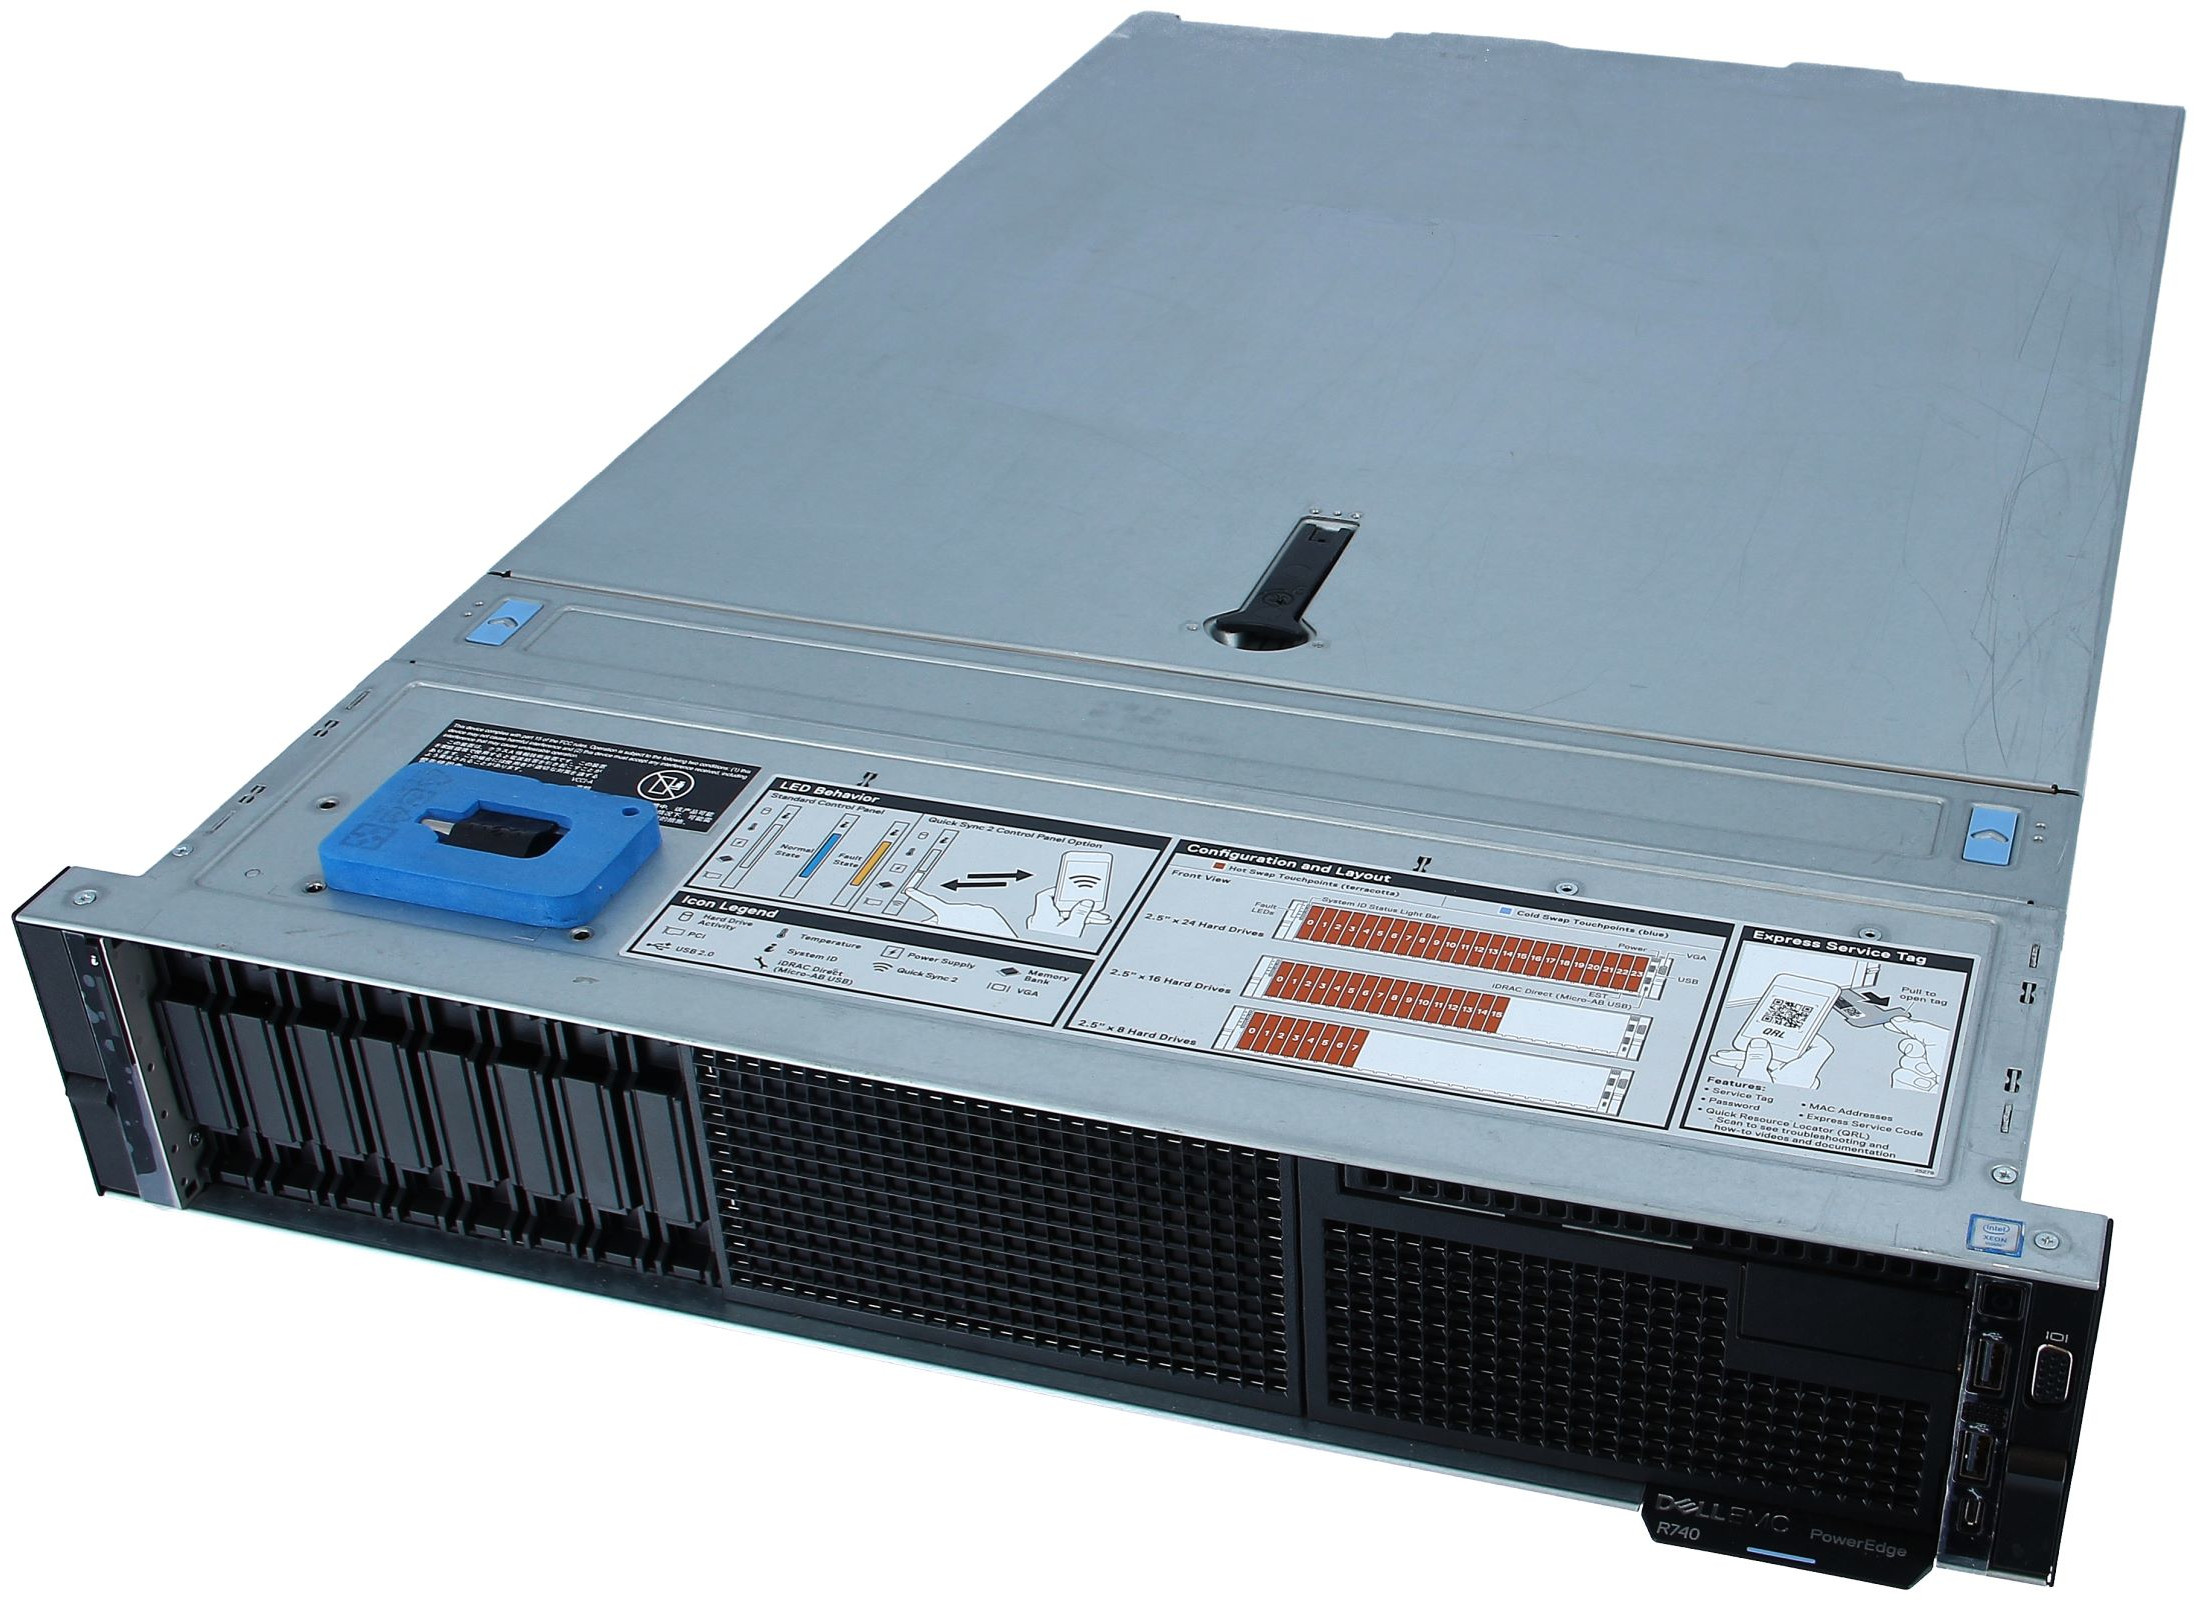
\includegraphics[width=3cm]{dell1}};
      \node[inner sep=2pt, draw] at ( 0, -2) (Pj) {$P_j$};
      \draw (Pj) -- (0, -2.5);
      \draw[fill=green] (-1, -2.5) rectangle (1, -7);

      \draw[fill=red]   (-1, -4.9) rectangle +(2, -1.1);
      \draw[fill=yellow!50] (-0.9, -5) rectangle node {data} +(1.8, -1);
      \draw[thick] (1.2, -4.9) -- node[anchor=west] {\mintinline{C}{MPI_Recv}} +(0, -1.1);
    \end{scope}

    \draw[ultra thick, ->] (1, -3.5) -| (2, -4);
    \draw[ultra thick, ->] (3.5, -4.6) -- ++(1, 0) -- (5, -5.5) -- ++(1, 0);
  \end{tikzpicture}  
\end{frame}

%%%%%%%%%%%%%%%%%%%%%%%%%%%%%%%%%%%%%%%%%%%%%%%%%%%%%%%%%%%%%%%%%%%%%%%%%%%%%%%%%%%%%%%%%%%%%

\begin{frame}
  \frametitle{Summary}

  \begin{exampleblock}{Blocking / Non-blocking}
    \begin{itemize}
    \item blocking send: send buffer can be overwritten
    \item blocking Receive: data is ready in receive buffer
    \item non-blocking: buffer must not be touched until completion
    \end{itemize}
  \end{exampleblock}
  
  \begin{alertblock}{Send: Synchronous / Buffered / Standard}
    \begin{itemize}
    \item Buffered: may complete before a matching receive is posted
      \begin{itemize}
      \item Needs more memory
      \end{itemize}
    \item Synchronous: completes only if a matching receive started
      \begin{itemize}
      \item No need for additional memory
      \item \textbf{Synchronizes} processes
        
      \end{itemize}
    \item Standard: either Buffered or Synchronous (best perf.) 
    \end{itemize}
  \end{alertblock}
\end{frame}

%%%%%%%%%%%%%%%%%%%%%%%%%%%%%%%%%%%%%%%%%%%%%%%%%


\begin{frame}[fragile=singleslide]
  \frametitle{Non-Blocking Functions}

\begin{minted}[fontsize=\small]{C}
int MPI_Isend(void* buf, int count, MPI_Datatype datatype,
              int dest, int tag, MPI_Comm comm,
              MPI_Request *request)

int MPI_Irecv(void* buf, int count, MPI_Datatype datatype,
             int source, int tag, MPI_Comm comm,
             MPI_Request *request)

int MPI_Wait(MPI_Request *request, MPI_Status *status)
\end{minted}

  \begin{block}{Rules}
    \begin{itemize}
    \item Non-blocking operations use resources
      \begin{itemize}
      \item Maintain state in an \mintinline{C}{MPI_Request}
      \end{itemize}
    \item They \textbf{must} be waited for
      \begin{itemize}
      \item \mintinline{C}{MPI_Wait} releases resources 
      \item Buffer can be read/overwritten after waiting
      \end{itemize}
    \end{itemize}
  \end{block}
\end{frame}

%%%%%%%%%%%%%%%%%%%%%%%%%%%%%%%%%%%%%%%

%%%%%%%%%%%%%%%%%%%%%%%%%%%%%%%%%%%%%%%%%%%%%%%%%%%%%%%%%%%%%%%%%

\begin{frame}[fragile]
\frametitle{MPI : Simultanenous Send / Receive}

\begin{itemize}
\item Recurring pattern
  \begin{itemize}
  \item Shift operation across a chain of processes
  \end{itemize}
\item Naive solution (\mintinline{C}{MPI_Send; MPI_Recv}) $\leadsto$ \alert{$\skull$ deadlock $\skull$}
\end{itemize}

\medskip

\begin{minted}[fontsize=\scriptsize]{C}
int MPI_Sendrecv(void *sendbuf, int sendcount, MPI_Datatype sendtype,
                 int dest, int sendtag,
                 void *recvbuf, int recvcount, MPI_Datatype recvtype,
                 int source, int recvtag,
                 MPI_Comm comm, MPI_Status *status);
\end{minted}

\begin{itemize}
\item \mintinline{C}{source == dest} is legal
\item The send and receive buffers must not overlap
\end{itemize}
%Les deux buffer doivent être distincts et ne pas se chevaucher.

\medskip

\begin{minted}[fontsize=\scriptsize]{C}
int MPI_Sendrecv_replace(void* buf, int count, MPI_Datatype datatype,
                         int dest, int sendtag, int source, int recvtag,
                         MPI_Comm comm, MPI_Status *status);
\end{minted}

\begin{itemize}
\item May allocate memory
\end{itemize}
\end{frame}

%%%%%%%%%%%%%%%%%%%%%%%%%%%%%%%%%%%%%%%%%%%%%%%%%%%%%%%%%%%%%%%%%%%%%%%%%%%%%%%%%%%%%%

\begin{frame}
  \frametitle{Collective Operations}

  \begin{itemize}
  \item Point-to-Point operations (two processes) 
  \item Collective operations (\alert{all} processes)
    \begin{itemize}
    \item Broadcast, Gather, Scatter, Reduction, ...
    \end{itemize}
  \end{itemize}

  \bigskip
  
  \begin{block}{Rule}
    \begin{itemize}
    \item Collective communications take place in a communicator
    \item All processes of a communicator \textbf{MUST} call the function
      \begin{itemize}
      \item It requires some action from them
      \item They can't do it if you don't allow them to
      \end{itemize}
    \end{itemize}
  \end{block}
\end{frame}

%%%%%%%%%%%%%%%%%%%%%%%%%%%%%%%%%%%%%%%%%%%%%%%%%%%%%%%%%%%%%%%%%

\begin{frame}[fragile=singleslide]
\frametitle{Broadcast}

\begin{minted}[fontsize=\footnotesize]{C}
int MPI_Bcast(void* buffer, int count, MPI_Datatype datatype, 
              int root, MPI_Comm comm);
\end{minted}

\medskip

  \begin{center}
    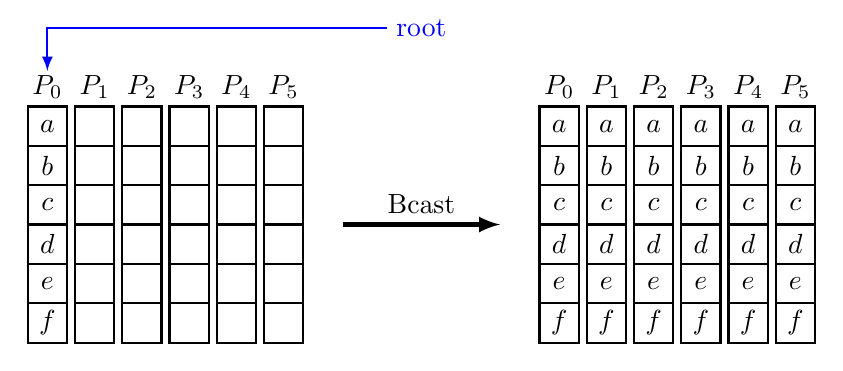
\begin{tikzpicture}[scale=0.5, >=latex]
      \path[use as bounding box] (0, 0) rectangle (20, 8);
  
      \node[blue] at (10, 8) (root) {root};
      \draw[thick, blue, ->] (root) -| (0.5, 6.9);
 
      \begin{scope}
        \foreach \i in {0,1,...,5} {
          \draw[thick] (1.2*\i, 0) rectangle +(1, 6);
          \foreach \j in {1,...,5} {
            \draw[thick] (1.2*\i, \j) -- +(1, 0);
          }
          \node at (1.2*\i + 0.5, 6.5) {$P_\i$};
        }
        \node at (0.5,  5.5) {$a$};
        \node at (0.5,  4.5) {$b$};
        \node at (0.5,  3.5) {$c$};
        \node at (0.5,  2.5) {$d$};
        \node at (0.5,  1.5) {$e$};
        \node at (0.5,  0.5) {$f$};
      \end{scope}
      
      \draw[ultra thick,->] (8, 3) -- node[above] {Bcast} (12, 3);
      
      \begin{scope}[xshift=13cm]
        \foreach \i in {0,1,...,5} {
          \draw[thick] (1.2*\i, 0) rectangle +(1, 6);
          \foreach \j in {1,...,5} {
            \draw[thick] (1.2*\i, \j) -- +(1, 0);
          }
          \node at (1.2*\i + 0.5, 6.5) {$P_\i$};
          \node at (1.2*\i + 0.5,  5.5) {$a$};
          \node at (1.2*\i + 0.5,  4.5) {$b$};
          \node at (1.2*\i + 0.5,  3.5) {$c$};
          \node at (1.2*\i + 0.5,  2.5) {$d$};
          \node at (1.2*\i + 0.5,  1.5) {$e$};
          \node at (1.2*\i + 0.5,  0.5) {$f$};
        }
      \end{scope}
    \end{tikzpicture}
  \end{center}

  \begin{block}{Remark}
    \begin{itemize}
    \item All processes must know \mintinline{C}{count} in advance
      \begin{itemize}
      \item Do \mintinline{C}{MPI_Bcast} with a single \mintinline{C}{int} first
      \end{itemize}
    \end{itemize}
  \end{block}
\end{frame}


%%%%%%%%%%%%%%%%%%%%%%%%%%%%%%%%%%%%%%%%%%%%%%%%%%%%%%%%%%%%%%%%%

\begin{frame}[fragile=singleslide]
  \frametitle{Gather / Scatter}

  \begin{wider}
\begin{minted}[fontsize=\footnotesize]{C}
int MPI_Gather(void* sendbuf, int sendcount, MPI_Datatype sendtype,
               void* recvbuf, int recvcount, MPI_Datatype recvtype,
               int root, MPI_Comm comm);

int MPI_Scatter(void* sendbuf, int sendcount, MPI_Datatype sendtype,
                void* recvbuf, int recvcount, MPI_Datatype recvtype,
                int root, MPI_Comm comm);
\end{minted}
  \end{wider}

  \medskip

\begin{center}
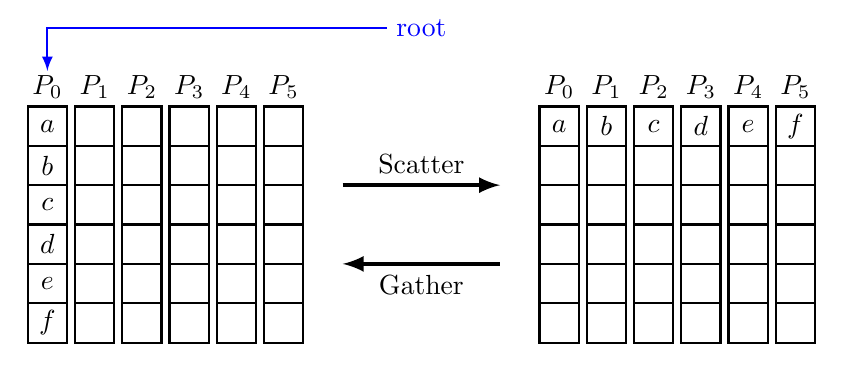
\begin{tikzpicture}[scale=0.5, >=latex]
  \path[use as bounding box] (0, 0) rectangle (20, 8);
  
  \node[blue] at (10, 8) (root) {root};
  \draw[thick, blue, ->] (root) -| (0.5, 6.9);
 
%%%%%%%%%%%% Scatter / Gather
  \begin{scope}
    \foreach \i in {0,1,...,5} {
      \draw[thick] (1.2*\i, 0) rectangle +(1, 6);
      \foreach \j in {1,...,5} {
        \draw[thick] (1.2*\i, \j) -- +(1, 0);
      }
      \node at (1.2*\i + 0.5, 6.5) {$P_\i$};
    }
  \node at (0.5,  5.5) {$a$};
  \node at (0.5,  4.5) {$b$};
  \node at (0.5,  3.5) {$c$};
  \node at (0.5,  2.5) {$d$};
  \node at (0.5,  1.5) {$e$};
  \node at (0.5,  0.5) {$f$};
  \end{scope}
  
\draw[ultra thick,->] (8, 4) -- node[above] {Scatter} (12, 4);
\draw[ultra thick,<-] (8, 2) -- node[below] {Gather} (12, 2);

\begin{scope}[xshift=13cm]
   \foreach \i in {0,1,...,5} {
      \draw[thick] (1.2*\i, 0) rectangle +(1, 6);
      \foreach \j in {1,...,5} {
        \draw[thick] (1.2*\i, \j) -- +(1, 0);
      }
      \node at (1.2*\i + 0.5, 6.5) {$P_\i$};
    }
    \node at (0.5,  5.5) {$a$};
    \node at (1.7,  5.5) {$b$};
    \node at (2.9,  5.5) {$c$};
    \node at (4.1,  5.5) {$d$};
    \node at (5.3,  5.5) {$e$};
    \node at (6.5,  5.5) {$f$};
      \end{scope}
    \end{tikzpicture}
  \end{center}
\end{frame}

%%%%%%%%%%%%%%%%%%%%%%%%%%%%%%%%%%%%%%%%%%%%%%%%%%

\begin{frame}[fragile=singleslide]
  \frametitle{Gather / Scatter}
  \framesubtitle{Comments about the Arguments}
  
  \begin{exampleblock}{Some arguments only make sense when \mintinline{C}{rank == root}}
    \begin{itemize}
    \item Gather: the receive buffer
    \item Scatter: the send buffer
    \item \textbf{Ignored} otherwise
    \end{itemize}
  \end{exampleblock}

  \begin{block}{Important point}
    \begin{itemize}
    \item \mintinline{C}{recvcount == sendcount} = \#elements \textbf{per process}
    \end{itemize}
  \end{block}
  
  \begin{alertblock}{\mintinline{C}{root} \textbf{Copy} \mintinline{C}{count}
      items from \mintinline{C}{sendbuf} to \mintinline{C}{recvbuf}}
    \begin{itemize}
    \item Can be disabled with \mintinline{C}{sendbuf == MPI_IN_PLACE}
      \begin{itemize}
      \item Ignore send buffer
      \item ``own'' data \textbf{already} at the right place in the receive buffer
      \end{itemize}
    \end{itemize}
  \end{alertblock}
\end{frame}

%%%%%%%%%%%%%%%%%%%%%%%%%%%%%%%%%%%%%%%%%%%%%%%%%%

\begin{frame}[fragile=singleslide]
  \frametitle{Gather / Scatter}
  \framesubtitle{Comments about array sizes}
  
  \begin{alertblock}{Big array divided into \textbf{equally sized} slices}
    \begin{itemize}
    \item \mintinline{C}{count} elements per process
    \item \mintinline{C}{p} processes
    \item Total size of the array is \mintinline{C}{count} $\times$ \mintinline{C}{p}
    \end{itemize}
  \end{alertblock}
  
  \begin{block}{Potential mismatch}
    \begin{itemize}
    \item \#process imposed by the \textbf{hardware}
    \item Array size imposed by \textbf{user input}
    \end{itemize}
  \end{block}
  
  \begin{exampleblock}{Two potential solutions}
    \begin{enumerate}
    \item Padding
    \item \mintinline{C}{MPI_Gatherv} and \mintinline{C}{MPI_Scatterv}
    \end{enumerate}
  \end{exampleblock}
\end{frame}


%%%%%%%%%%%%%%%%%%%%%%%%%%%%%%%%%%%%%%%%%%%%%%%%%% 

\begin{frame}[fragile=singleslide]
  \frametitle{Array of Size $n$ Must be Divided in $p$ Slices}

  \begin{block}{Idea \#1: pad the array}
    \begin{itemize}
    \item Slices of size $k = \lceil n / p \rceil = \mintinline{C}{(n + p - 1) / p}$
    \item Allocate a (larger) array $A$ of size $kp$
    \item Only \mintinline{python}{A[0:n]} contains meaningful data
    \end{itemize}

    \begin{center}
      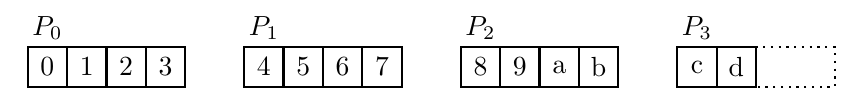
\begin{tikzpicture}[scale=0.5]
        \path[use as bounding box] (0, 0.5) rectangle (20.5, 1.5);
      \draw[thick] (0, 0) rectangle +(4, 1);
      \draw[thick] (1, 0) -- +(0, 1);
      \draw[thick] (2, 0) -- +(0, 1);
      \draw[thick] (3, 0) -- +(0, 1);
      \node at (0.5, 0.5) {0};
      \node at (1.5, 0.5) {1};
      \node at (2.5, 0.5) {2};
      \node at (3.5, 0.5) {3};
      \node at (0.5, 1.5) {$P_0$};

      \begin{scope}[xshift=5.5cm]
        \draw[thick] (0, 0) rectangle +(4, 1);
        \draw[thick] (1, 0) -- +(0, 1);
        \draw[thick] (2, 0) -- +(0, 1);
        \draw[thick] (3, 0) -- +(0, 1);
        \node at (0.5, 0.5) {4};
        \node at (1.5, 0.5) {5};
        \node at (2.5, 0.5) {6};
        \node at (3.5, 0.5) {7};
        \node at (0.5, 1.5) {$P_1$};
      \end{scope}

      \begin{scope}[xshift=11cm]
        \draw[thick] (0, 0) rectangle +(4, 1);
        \draw[thick] (1, 0) -- +(0, 1);
        \draw[thick] (2, 0) -- +(0, 1);
        \draw[thick] (3, 0) -- +(0, 1);
        \node at (0.5, 0.5) {8};
        \node at (1.5, 0.5) {9};
        \node at (2.5, 0.5) {a};
        \node at (3.5, 0.5) {b};
        \node at (0.5, 1.5) {$P_2$};
      \end{scope}

      \begin{scope}[xshift=16.5cm]
        \draw[thick] (0, 0) rectangle +(2, 1);
        \draw[dotted,thick] (2, 0) rectangle +(2, 1);
        \draw[thick] (1, 0) -- +(0, 1);
        \node at (0.5, 0.5) {c};
        \node at (1.5, 0.5) {d};
        \node at (0.5, 1.5) {$P_3$};
      \end{scope}
    \end{tikzpicture}
  \end{center}

  \end{block}

  \begin{alertblock}{Alternative}
    \begin{itemize}
    \item Process $i$ has \mintinline{python}{A[i*n/p : (i+1)*n/p]}
    \end{itemize}

    \begin{center}
    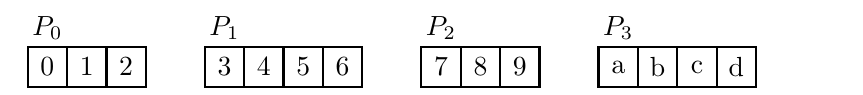
\begin{tikzpicture}[scale=0.5]
        \path[use as bounding box] (0, 0.5) rectangle (20.5, 1.5);
      \draw[thick] (0, 0) rectangle +(3, 1);
      \draw[thick] (1, 0) -- +(0, 1);
      \draw[thick] (2, 0) -- +(0, 1);
      \node at (0.5, 0.5) {0};
      \node at (1.5, 0.5) {1};
      \node at (2.5, 0.5) {2};
      \node at (0.5, 1.5) {$P_0$};

      
      \draw[thick] (4.5, 0) rectangle +(4, 1);
      \draw[thick] (5.5, 0) -- +(0, 1);
      \draw[thick] (6.5, 0) -- +(0, 1);
      \draw[thick] (7.5, 0) -- +(0, 1);
      \node at (5, 0.5) {3};
      \node at (6, 0.5) {4};
      \node at (7, 0.5) {5};
      \node at (8, 0.5) {6};
      \node at (5, 1.5) {$P_1$};
      
      \draw[thick] (10, 0) rectangle +(3, 1);
      \draw[thick] (11, 0) -- +(0, 1);
      \draw[thick] (12, 0) -- +(0, 1);
      \node at (10.5, 0.5) {7};
      \node at (11.5, 0.5) {8};
      \node at (12.5, 0.5) {9};
      \node at (10.5, 1.5) {$P_2$};

      \draw[thick] (14.5, 0) rectangle +(4, 1);
      \draw[thick] (15.5, 0) -- +(0, 1);
      \draw[thick] (16.5, 0) -- +(0, 1);
      \draw[thick] (17.5, 0) -- +(0, 1);
      \node at (15, 0.5) {a};
      \node at (16, 0.5) {b};
      \node at (17, 0.5) {c};
      \node at (18, 0.5) {d};
      \node at (15, 1.5) {$P_3$};
    \end{tikzpicture}
  \end{center}
  \begin{itemize}
  \item Requires the use of \mintinline{C}{MPI_Gatherv}, \mintinline{C}{MPI_Scatterv}
  \end{itemize}
\end{alertblock}
\end{frame}


%%%%%%%%%%%%%%%%%%%%%%%%%%%%%%%%%%%%%%%%%%%%%%%%%%% 

\begin{frame}[fragile]
\frametitle{Gather-to-All}

  \begin{wider}
\begin{minted}[fontsize=\footnotesize]{C}
int MPI_Allgather(void* sendbuf, int sendcount, MPI_Datatype sendtype,
                  void* recvbuf, int recvcount, MPI_Datatype recvtype, 
                  MPI_Comm comm);
\end{minted}
  \end{wider}

  \medskip

  \begin{center}
    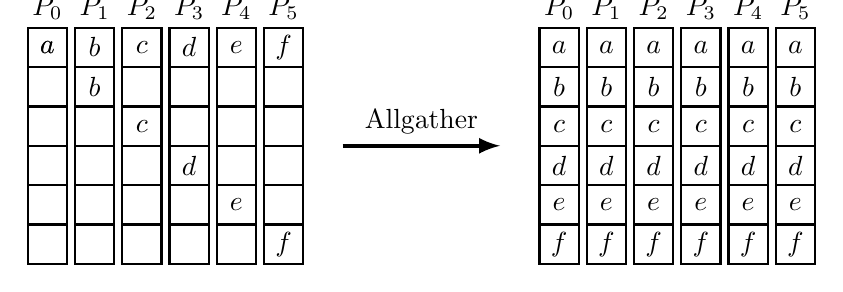
\begin{tikzpicture}[scale=0.5, >=latex]
      \path[use as bounding box] (0, 0) rectangle (20, 6);
      
      \begin{scope}
        \foreach \i in {0,1,...,5} {
          \draw[thick] (1.2*\i, 0) rectangle +(1, 6);
          \foreach \j in {1,...,5} {
            \draw[thick] (1.2*\i, \j) -- +(1, 0);
          }
          \node at (1.2*\i + 0.5, 6.5) {$P_\i$};
        }
        \node<1> at (0.5,  5.5) {$a$};
        \node<1> at (1.7,  5.5) {$b$};
        \node<1> at (2.9,  5.5) {$c$};
        \node<1> at (4.1,  5.5) {$d$};
        \node<1> at (5.3,  5.5) {$e$};
        \node<1> at (6.5,  5.5) {$f$};

        % IN-place
        \node<2> at (0.5,  5.5) {$a$};
        \node<2> at (1.7,  4.5) {$b$};
        \node<2> at (2.9,  3.5) {$c$};
        \node<2> at (4.1,  2.5) {$d$};
        \node<2> at (5.3,  1.5) {$e$};
        \node<2> at (6.5,  0.5) {$f$};
      \end{scope}
      
      \draw[ultra thick,->] (8, 3) -- node[above] {Allgather} (12, 3);
      
      \begin{scope}[xshift=13cm]
        \foreach \i in {0,1,...,5} {
          \draw[thick] (1.2*\i, 0) rectangle +(1, 6);
          \foreach \j in {1,...,5} {
            \draw[thick] (1.2*\i, \j) -- +(1, 0);
          }
          \node at (1.2*\i + 0.5, 6.5) {$P_\i$};
          \node at (1.2*\i + 0.5,  5.5) {$a$};
          \node at (1.2*\i + 0.5,  4.5) {$b$};
          \node at (1.2*\i + 0.5,  3.5) {$c$};
          \node at (1.2*\i + 0.5,  2.5) {$d$};
          \node at (1.2*\i + 0.5,  1.5) {$e$};
          \node at (1.2*\i + 0.5,  0.5) {$f$};
        }
      \end{scope}
    \end{tikzpicture}
  \end{center}
  
  \begin{itemize}
  \item See also : \mintinline{C}{MPI_Allgatherv}

    \pause
    
  \item \mintinline{C}{sendbuf == MPI_IN_PLACE} (for all processes)
    \begin{itemize}
    \item Send buffers ignored
    \item \textbf{Read} from the \textbf{receive} buffers
    \end{itemize}
  \end{itemize}
\end{frame}



%%%%%%%%%%%%%%%%%%%%%%%%%%%%%%%%%%%%%%%%%%%%%%%%%%%%

\begin{frame}[fragile=singleslide]
  \frametitle{All-to-All Scatter/Gather}

  \begin{wider}
\begin{minted}[fontsize=\footnotesize]{C}
int MPI_Alltoall(void* sendbuf, int sendcount, MPI_Datatype sendtype,
                 void* recvbuf, int recvcount, MPI_Datatype recvtype,
                 MPI_Comm comm);
\end{minted}
  \end{wider}  

  \bigskip

  \begin{center}
    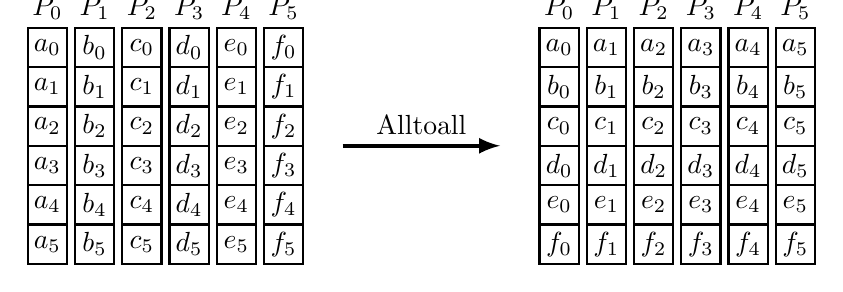
\begin{tikzpicture}[scale=0.5, >=latex]
      \path[use as bounding box] (0, 0) rectangle (20, 6);
      
      \begin{scope}
        \foreach \letter / \i in {a / 0, b / 1, c / 2, d / 3, e / 4, f / 5} {
          \draw[thick] (1.2*\i, 0) rectangle +(1, 6);
          \foreach \j in {1,...,5} {
            \draw[thick] (1.2*\i, \j) -- +(1, 0);
          }
          \node at (1.2*\i + 0.5, 6.5) {$P_\i$};
          \foreach \j in {0,1,...,5} {
            \node<1> at (0.5 + 1.2*\i,  5.5 - \j) {$\letter_\j$};
          }
        }
      \end{scope}
      
      \draw[ultra thick,->] (8, 3) -- node[above] {Alltoall} (12, 3);
      
      \begin{scope}[xshift=13cm]
        \foreach \letter / \i in {a / 0, b / 1, c / 2, d / 3, e / 4, f / 5} {
          \draw[thick] (1.2*\i, 0) rectangle +(1, 6);
          \foreach \j in {1,...,5} {
            \draw[thick] (1.2*\i, \j) -- +(1, 0);
          }
          \node at (1.2*\i + 0.5, 6.5) {$P_\i$};
          \foreach \j in {0,1,...,5} {
            \node<1> at (0.5 + 1.2*\j,  5.5 - \i) {$\letter_\j$};
          }
        }
      \end{scope}
    \end{tikzpicture}
  \end{center}
  
  \begin{itemize}
  \item See also : \mintinline{C}{MPI_Alltoallv}, \mintinline{C}{MPI_Alltoallw}
  \item \mintinline{C}{sendbuf == MPI_IN_PLACE} (for all processes)
    \begin{itemize}
    \item Send buffers ignored
    \item \textbf{receive} buffer sent then overwritten with received data
    \end{itemize}

  \end{itemize}
\end{frame}

%%%%%%%%%%%%%%%%%%%%%%%%%%%%%%%%%%%%%%%%%%%%%%%%%%%%

\begin{frame}[fragile]
\frametitle{Network Torture Test}

  \begin{wider}
\begin{minted}[fontsize=\footnotesize]{C}
int MPI_Alltoall(void* sendbuf, int sendcount, MPI_Datatype sendtype,
                 void* recvbuf, int recvcount, MPI_Datatype recvtype,
                 MPI_Comm comm);
\end{minted}
  \end{wider}

  \begin{alertblock}{Settings}
    \begin{itemize}  
    \item 16 nodes, 4GB per node (64GB in total)
    \item[$\leadsto$] Each node sends/receives 256MB to each other node
    \end{itemize}
  \end{alertblock}

\bigskip

\footnotesize 
\begin{tabular}{|c|c|c|l|r|r|}
  \hline
  Cluster & Site & Year & Interface & T & aggregated BW \\
  \hline
  \hline
  PPTI      & jussieu & 20?? & \phantom{00}1Gbit ethernet & 254s & 250Mo/s \\
  \pause
  sagitaire & lyon  & 2006 & \phantom{00}1Gbit ethernet   & ? &  \\
  \pause
  paravance & rennes & 2015 & \phantom{0}10Gbit ethernet   & 14.9s & 4Go/s \\
  \pause
  gros      & nancy & 2019 & \phantom{0}25Gbit ethernet   & 6.8s & 9.4Go/s \\
  \pause
  grcinq    & nancy & 2013 & \phantom{0}56Gbit InfiniBand & 4.8s & 13Go/s\\
  \pause
  grvingt   & nancy & 2018 & 100Gbit OmniPath             & 2.2s & 29Go/s \\
  \hline
\end{tabular}
\end{frame}

%%%%%%%%%%%%%%%%%%%%%%%%%%%%%%%%%%%%%%%%%%%%%%%%%%%%

\begin{frame}[fragile]
  \frametitle{Network Torture Test}
  \framesubtitle{With \emph{real} HPC hardware}

  \begin{wider}
\begin{minted}[fontsize=\footnotesize]{C}
int MPI_Alltoall(void* sendbuf, int sendcount, MPI_Datatype sendtype,
                 void* recvbuf, int recvcount, MPI_Datatype recvtype,
                 MPI_Comm comm);
\end{minted}
  \end{wider}

    \begin{itemize}  
    \item $n$ nodes, 6.75GB per node, $6.75n$GB in total
    \end{itemize}
 
\medskip

\footnotesize
\begin{overlayarea}{\textwidth}{5cm}
  \centering
  
  \only<1>{
    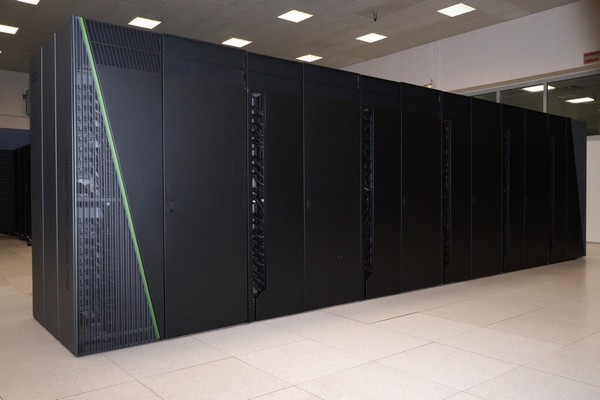
\includegraphics[height=5cm]{turing}
  }
  \begin{onlyenv}<2>
    \begin{tabular}{|r|r|r|r|}
  \hline
  \# nodes & Data             & T (s)        & Aggregated BW \\
  \hline\hline
  2        & 13.5GB           & 2.7      & 6.8GB/s \\
  4        & 27GB             & 2.9      & 9.3GB/s \\
    \vdots & \vdots           & \vdots   & \vdots  \\                                         
  64       & 430GB            & 4.1      & 105GB/s \\
  128      & 861GB            & 8.9      &  96GB/s \\
  256      & 1.7TB            & 13.0     & 130GB/s \\
  512      & 3.4TB            & 13.7     & 248GB/s \\
  1024     & 6.9TB            & 15.9     & 434GB/s \\
  2048     & 13.4TB           & 17.0     & 788GB/s \\
  4096     & 27.5TB           & 18.7     & 1470GB/s \\
    \hline
    \end{tabular}
  \end{onlyenv}
\end{overlayarea}

\end{frame}



%%%%%%%%%%%%%%%%%%%%%%%%%%%%%%%%%%%%%%%%%%%%%%%%%%%%

\begin{frame}[fragile=singleslide]
\frametitle{Reduce}

\begin{minted}[fontsize=\footnotesize]{C}
int MPI_Reduce(void *sendbuf, void *recvbuf, int count,
               MPI_Datatype datatype, MPI_Op op, int root,
               MPI_Comm comm);
\end{minted}
               
\bigskip

  \begin{center}
    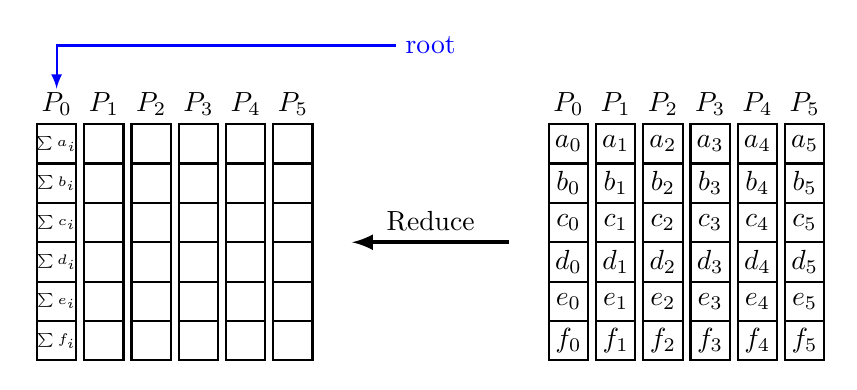
\begin{tikzpicture}[scale=0.5, >=latex]
      \node[blue] at (10, 8) (root) {root};
      \draw[thick, blue, ->] (root) -| (0.5, 6.9);

      \begin{scope}
        \foreach \letter / \i in {a / 0, b / 1, c / 2, d / 3, e / 4, f / 5} {
          \draw[thick] (1.2*\i, 0) rectangle +(1, 6);
          \foreach \j in {1,...,5} {
            \draw[thick] (1.2*\i, \j) -- +(1, 0);
          }
          \node at (1.2*\i + 0.5, 6.5) {$P_\i$};          
          \node at (0.5, 5.5 - \i) {$\scriptscriptstyle \sum \letter_i$};
        }
      \end{scope}
      
      \draw[ultra thick,<-] (8, 3) -- node[above] {Reduce} (12, 3);

      \begin{scope}[xshift=13cm]
        \foreach \letter / \i in {a / 0, b / 1, c / 2, d / 3, e / 4, f / 5} {
          \draw[thick] (1.2*\i, 0) rectangle +(1, 6);
          \foreach \j in {1,...,5} {
            \draw[thick] (1.2*\i, \j) -- +(1, 0);
          }
          \node at (1.2*\i + 0.5, 6.5) {$P_\i$};
          \foreach \j in {0,1,...,5} {
            \node<1> at (0.5 + 1.2*\j,  5.5 - \i) {$\letter_\j$};
          }
        }
      \end{scope}
    \end{tikzpicture}
  \end{center}
  
  \begin{itemize}
  \item \mintinline{C}{sendbuf == MPI_IN_PLACE} works at \mintinline{C}{root}
  \item Predefined operations: $+$, $\times$, $\min$, $\max$, AND, OR, XOR, ...  
  \item User-definable operations
  \end{itemize}
\end{frame}

%%%%%%%%%%%%%%%%%%%%%%%%%%%%%%%%%%%%%%%%%%%%%%%%%

\begin{frame}[fragile=singleslide]
\frametitle{All-Reduce}

  \begin{wider}
    \begin{minted}[fontsize=\footnotesize]{C}
int MPI_Allreduce(void *sendbuf, void *recvbuf, int count,
                 MPI_Datatype datatype, MPI_Op op, MPI_Comm comm);
               \end{minted}
  \end{wider}  

  \bigskip

  \begin{center}
    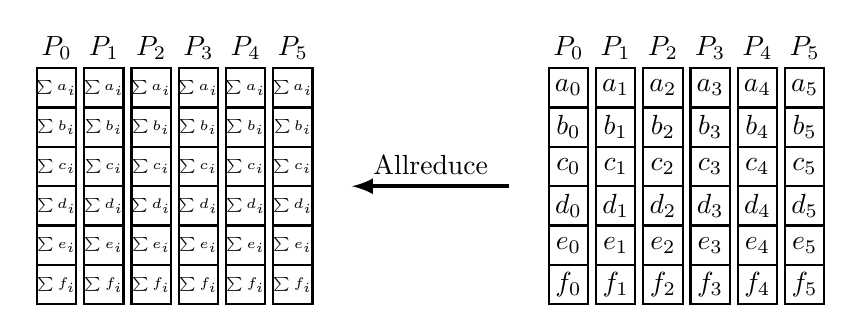
\begin{tikzpicture}[scale=0.5, >=latex]
      \begin{scope}
        \foreach \letter / \i in {a / 0, b / 1, c / 2, d / 3, e / 4, f / 5} {
          \draw[thick] (1.2*\i, 0) rectangle +(1, 6);
          \foreach \j in {1,...,5} {
            \draw[thick] (1.2*\i, \j) -- +(1, 0);
          }
          \node at (1.2*\i + 0.5, 6.5) {$P_\i$};          
          \foreach \j in {0,...,5} {
            \node at (0.5 + 1.2*\j, 5.5 - \i) {$\scriptscriptstyle \sum \letter_i$};
          }
        }
      \end{scope}
      
      \draw[ultra thick,<-] (8, 3) -- node[above] {Allreduce} (12, 3);

      \begin{scope}[xshift=13cm]
        \foreach \letter / \i in {a / 0, b / 1, c / 2, d / 3, e / 4, f / 5} {
          \draw[thick] (1.2*\i, 0) rectangle +(1, 6);
          \foreach \j in {1,...,5} {
            \draw[thick] (1.2*\i, \j) -- +(1, 0);
          }
          \node at (1.2*\i + 0.5, 6.5) {$P_\i$};
          \foreach \j in {0,1,...,5} {
            \node<1> at (0.5 + 1.2*\j,  5.5 - \i) {$\letter_\j$};
          }
        }
      \end{scope}
    \end{tikzpicture}
  \end{center}

    \begin{itemize}
  \item \mintinline{C}{sendbuf == MPI_IN_PLACE} works (all processes)
  \item Predefined operations: $+$, $\times$, $\min$, $\max$, AND, OR, XOR, ...  
  \item User-definable operations
  \end{itemize}
\end{frame}

%%%%%%%%%%%%%%%%%%%%%%%%%%%%%%%%%%%%%%%%%%%%%%%%%%%%%%%%%%%%%%%%

\begin{frame}[fragile=singleslide]
  \frametitle{Reduce-Scatter}

  \begin{wider}
\begin{minted}[fontsize=\footnotesize]{C}
int MPI_Reduce_scatter_block(void* sendbuf, void* recvbuf,
                             int recvcount, MPI_Datatype datatype,
                             MPI_Op op, MPI_Comm comm)
\end{minted}
  \end{wider}

  \bigskip

  \begin{center}
    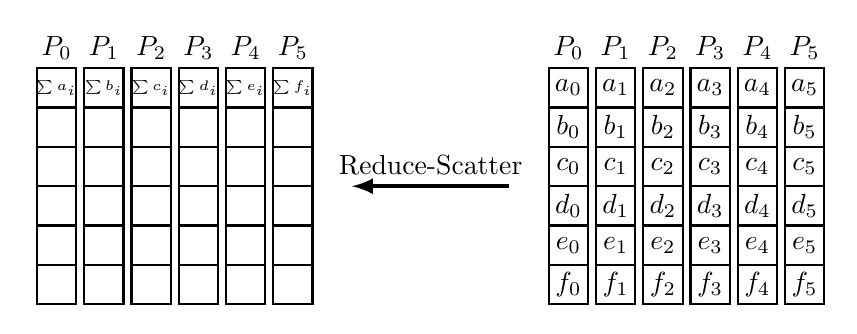
\begin{tikzpicture}[scale=0.5, >=latex]
            \begin{scope}
        \foreach \letter / \i in {a / 0, b / 1, c / 2, d / 3, e / 4, f / 5} {
          \draw[thick] (1.2*\i, 0) rectangle +(1, 6);
          \foreach \j in {1,...,5} {
            \draw[thick] (1.2*\i, \j) -- +(1, 0);
          }
          \node at (1.2*\i + 0.5, 6.5) {$P_\i$};          
          \node at (0.5 + 1.2*\i, 5.5) {$\scriptscriptstyle \sum \letter_i$};
        }
      \end{scope}

      \draw[ultra thick,<-] (8, 3) -- node[above] {Reduce-Scatter} (12, 3);

      \begin{scope}[xshift=13cm]
        \foreach \letter / \i in {a / 0, b / 1, c / 2, d / 3, e / 4, f / 5} {
          \draw[thick] (1.2*\i, 0) rectangle +(1, 6);
          \foreach \j in {1,...,5} {
            \draw[thick] (1.2*\i, \j) -- +(1, 0);
          }
          \node at (1.2*\i + 0.5, 6.5) {$P_\i$};
          \foreach \j in {0,1,...,5} {
            \node<1> at (0.5 + 1.2*\j,  5.5 - \i) {$\letter_\j$};
          }
        }
      \end{scope}
\end{tikzpicture}
\end{center}

    \begin{itemize}
    \item \mintinline{C}{sendbuf == MPI_IN_PLACE} works (all processes)
    \item Predefined operations: $+$, $\times$, $\min$, $\max$, AND, OR, XOR, ...  
    \item User-definable operations
    \item See also : \mintinline{C}{MPI_Reduce_scatter}
    \end{itemize}
\end{frame}

%%%%%%%%%%%%%%%%%%%%%%%%%%%%%%%%%%%%%%%%%%%%%%%%%%%%%%%%%%%%%%%%%%%%%%%%%

\begin{frame}[fragile=singleslide]
\frametitle{Scan}
\framesubtitle{A.k.a. Prefix-sum}

\begin{minted}[fontsize=\footnotesize]{C}
int MPI_Scan(void* sendbuf, void* recvbuf, int count,
             MPI_Datatype datatype, MPI_Op op, MPI_Comm comm);
\end{minted}
  
\bigskip

\begin{center}
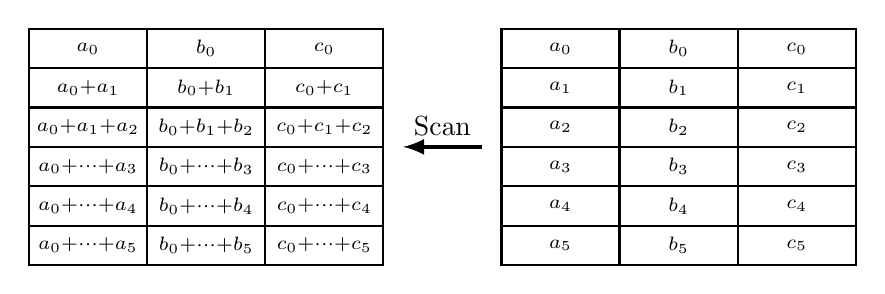
\begin{tikzpicture}[scale=0.5, >=latex]
  \begin{scope}
    \draw[thick] (0, 0) rectangle +(9, 6);
    \draw[thick] (3, 0) -- +(0, 6);
    \draw[thick] (6, 0) -- +(0, 6);
    \foreach \i in {0,1,...,6} {
      \draw[thick] (0, \i) -- +(9, 0);
    }
    
    \node at (1.5, 5.5) {$\scriptstyle a_0$};
    \node at (4.5, 5.5) {$\scriptstyle b_0$};
    \node at (7.5, 5.5) {$\scriptstyle c_0$};

    \node at (1.5, 4.5) {$\scriptstyle a_0 + a_1$};
    \node at (4.5, 4.5) {$\scriptstyle b_0 + b_1$};
    \node at (7.5, 4.5) {$\scriptstyle c_0 + c_1$};

    
    \node at (1.5, 3.5) {$\scriptstyle a_0 + a_1 + a_2$};
    \node at (4.5, 3.5) {$\scriptstyle b_0 + b_1 + b_2$};
    \node at (7.5, 3.5) {$\scriptstyle c_0 + c_1 + c_2$};

    \foreach \i in {3, 4, 5} {
      \node at (1.5, 5.5-\i) {$\scriptstyle a_0 + \dots + a_\i$};
      \node at (4.5, 5.5-\i) {$\scriptstyle b_0 + \dots + b_\i$};
      \node at (7.5, 5.5-\i) {$\scriptstyle c_0 + \dots + c_\i$};
    }
  \end{scope}

\draw[ultra thick,<-] (9.5, 3) -- node[above] {Scan} (11.5, 3);

\begin{scope}[xshift=12cm]
    \draw[thick] (0, 0) rectangle +(9, 6);
    \draw[thick] (3, 0) -- +(0, 6);
    \draw[thick] (6, 0) -- +(0, 6);
    \foreach \i in {0,1,...,6} {
      \draw[thick] (0, \i) -- +(9, 0);
    }

  \foreach \i in {0,1,...,5} {
    \node at (1.5, 5.5-\i) {$\scriptstyle a_\i$};
    \node at (4.5, 5.5-\i) {$\scriptstyle b_\i$};
    \node at (7.5, 5.5-\i) {$\scriptstyle c_\i$};
  }
\end{scope}
\end{tikzpicture}
\end{center}

    \begin{itemize}
    \item \mintinline{C}{sendbuf == MPI_IN_PLACE} works (all processes)
    \item Predefined operations: $+$, $\times$, $\min$, $\max$, AND, OR, XOR, ...  
    \item User-definable operations
    \item See also : \mintinline{C}{MPI_Exscan}
    \end{itemize}
\end{frame}

%%%%%%%%%%%%%%%%%%%%%%%%%%%%%%%%%%%%%%%%%%%%%%%%%%%%%%%%%%%%%%%%%%%%%%%%%%%%%%%%%%%%%%%%

\begin{frame}[fragile=singleslide]
  \frametitle{Guess What?}
  
  \begin{block}{\textbf{Non-blocking} collective operations \smiley}
    \begin{itemize}
    \item Only since MPI v3.0 (2012)
    \item \mintinline{C}{MPI_Ibcast}, \mintinline{C}{MPI_Iscatter}, \mintinline{C}{MPI_Igather}, \mintinline{C}{MPI_Iallgather}, \mintinline{C}{MPI_Ialltoall}, \mintinline{C}{MPI_Ireduce}, \mintinline{C}{MPI_Iallreduce}, \mintinline{C}{MPI_Ireduce_scatter}, etc.
    \end{itemize}
  \end{block}
\end{frame}

%%%%%%%%%%%%%%%%%%%%%%%%%%%%%%%%%%%%%%%%%%%%%%%%%%%%%%%%%%%%%%%%%%%%%%%%%%%%%%%%%%%%%%%%%%

\begin{frame}[fragile=singleslide]
  \frametitle{Collective Operations on a Subgroup}

  \begin{itemize}
  \item Collective operations $=$ all processes in a \alert{communicator}
  \item Initially, a single communicator (\mintinline{C}{MPI_COMM_WORLD})
  \item Possible to create \textbf{sub-}communicators
  \end{itemize}
  
\begin{minted}[fontsize=\footnotesize]{C}
int MPI_Comm_split(MPI_Comm comm, int color, int key,
                   MPI_Comm *newcomm);
\end{minted}

  \begin{block}{Description}
    \begin{itemize}
    \item Collective operation
    \item \mintinline{C}{newcomm} contains all processes in \mintinline{C}{comm} with the same \mintinline{C}{color}, ordered by \mintinline{C}{key} (ties broken with rank in \mintinline{C}{comm})
      \begin{itemize}
      \item This \textbf{partitions} \mintinline{C}{comm}
      \item Distinct sub-communicator for each value of \mintinline{C}{key}
      \end{itemize}
    \end{itemize}
  \end{block}
\end{frame}

%%%%%%%%%%%%%%%%%%%%%%%%%%%%%%%%%%%%%%%%%%%%%%%%%%%%%%%%%%%%%%%%%%%%%%%%%%%%%%%%%%%%%%%%

\begin{frame}[fragile]
  \frametitle{Typical Use-Case: 2D Process Grid}

  \begin{center}
    \begin{tikzpicture}
      \path[use as bounding box] (-0.25, 1) rectangle (9, -4);
      
      \foreach \i in {0, ..., 3} {
        \draw<2,4>[blue, thick, fill=blue, nearly transparent] (-1, -\i - 0.35) rectangle +(8, 0.7);
      }
      \foreach \j in {0, ..., 4} {
        \draw<3,4>[green, thick, fill=green, nearly transparent] (1.5cm*\j - 1.25em, 0.75) rectangle +(2.5em, -4.5);
      }

      \draw<1,4>[red, ultra thick] (-1.25, 1) rectangle +(8.5, -5);
      \node<1,4>[red, anchor=north west, inner sep=0] at (7.35, 1) {\mintinline{C}{MPI_COMM_WORLD}};
      
      \foreach \i in {0, ..., 3} {
        \foreach \j in {0, ..., 4} {
          \tikzmath{integer \k;
            \k = \i*5 + \j;
          }
          \node<1,4>[inner sep=2pt, draw, minimum width=2em] at (1.5*\j, -\i) {$P_{\k}$};
          \node<2>[inner sep=2pt, draw, minimum width=2em] at (1.5*\j, -\i) {$P_{\j}$};
          \node<3>[inner sep=2pt, draw, minimum width=2em] at (1.5*\j, -\i) {$P_{\i}$};
        }
      }

      \node<2,4>[blue, anchor=west, inner sep=0] at (8.5, -1.5) (rowcomm) {\mintinline{C}{rowcomm}};
      \foreach \i in {0, ..., 3} {
        \draw<2,4>[blue, ->] (rowcomm) -- +(-1, 0) |- ( 7, -\i);
      }
      
      \node<3,4>[green, anchor=west, inner sep=0] at (8.5, -3.5) (colcomm) {\mintinline{C}{colcomm}};
      \foreach \j in {0, ..., 4} {
        \draw<3,4>[green, thick, ->] (colcomm) -- +(0, -0.75) -| (1.5cm*\j, -3.75);
      }
     
    \end{tikzpicture}
  \end{center}

  \begin{minted}[fontsize=\small]{C}
    MPI_Comm rowcomm, colcomm;
    int i = rank / n, j = rank % n;
    MPI_Comm_split(MPI_COMM_WORLD, i, j, &rowcomm);
    MPI_Comm_split(MPI_COMM_WORLD, j, i, &colcomm);
  \end{minted}
  
  \begin{itemize}
  \item See also \mintinline{C}{MPI_Cart_create} and \mintinline{C}{MPI_Cart_Sub}
  \end{itemize}
\end{frame}

\end{document}

% Charles' emacs magic commands
%%% Local Variables:
%%% TeX-engine: xetex
%%% TeX-command-extra: "-shell-escape"
%%% TeX-command-extra-options: "-shell-escape"
%%% ispell-local-dictionary: "english"
%%% eval: (flyspell-mode 1)
%%% eval: (reftex-mode 1)
%%% End:
